\documentclass[12pt,openany]{book}
%\usepackage{classnotestikz}
%\usepackage{tikzelements}
\usepackage{libro-fciencias}
\usepackage{booktabs}
\usepackage{colortbl}
\def\thickline{\specialrule{.15em}{.05em}{.05em}}
\def\violetrule{\color{Violeta}{\rule{100px}{0.05em}}}
\def\bluerule{\color{DarkBlue}{\rule{100px}{0.05em}}}
\usepackage{multirow}


\usepackage{diagramas-fciencias}
\pgfplotsset{compat=1.15}

\graphicspath{ {Figuras/} }

%\setcounter{tocdepth}{4}

\addbibresource{rnnotesref.bib}


%----------------------------------------------------------------------------------------
%	Autores y Título
%----------------------------------------------------------------------------------------

\title{Redes Neuronales}
\subtitle{Notas de clase}
\author{Karla Fernanda Jiménez Gutiérrez\newline
        Verónica Esther Arriola Ríos}
\publisher{Facultad de Ciencias, UNAM}
\background{Neurona.png}


\begin{document}
\maketitle

%----------------------------------------------------------------------------------------
% Contenido
%----------------------------------------------------------------------------------------
\frontmatter % Numeración romana
\tableofcontents
\clearemptydoublepage % Whitespace to the end of the page


%----------------------------------------------------------------------------------------
%	                                Inicio
%----------------------------------------------------------------------------------------
\mainmatter  % Numeración arabiga


%%
\chapter*{Etc}

A lo largo del texto se utilizará la siguiente notación para diversos elementos:
\begin{longtable}{lc}
 Conjuntos   &   $\set{C}$ \\
 Vectores    &   $\vec{X}$ \\
 Matrices    &   $\mat{M}$ \\
 Unidades    &   $\unit{cm}$
\end{longtable}



%%
\part{Antecedentes}
\chapter{Neurona biológica}
\section{Neurociencias computacionales}

Las redes neuronales surgieron completamente inspiradas en los sistemas biológicos. 
Lo que estamos haciendo los computólogos es tomar una idea de la naturaleza, una idea que ha probado ser sumamente efectiva para procesar información y que logra resolver problemas que nosotros aún no sabemos solucionar con modelos diseñados explícitamente.
Los más notorios son: 
\begin{itemize}
\item Problemas de visión por computadora.
\item Procesamiento del lenguaje natural.
\end{itemize}

A lo largo del texto obtendremos una somera idea de qué hace el sistema nervioso de un ser humano, tomaremos también ejemplos de animales como el calamar gigante y cangrejos; ejemplos que han permitido estudiar biológicamente cómo funcionan las neuronas y cómo funciona su sistema nervioso. 

Entonces por un momento pensemos en el sistema nervioso como un todo, lo que realmente está pasando al computar no es el cálculo del proceso  de una sola neurona sino de la colección de todas ellas. Lo que sucede con los sistemas biológicos es que son muchísimo más complicados que lo que vamos a ver nosotros como modelos computacionales, sin embargo muchísimas empresas están utilizando estas técnicas. 
El sistema nervioso como un todo es bastante más complejo, pero conforme han ido evolucionando las redes neuronales computacionales, ya con sus arquitecturas y organizaciones, se están volviendo también más complejas. Varias de las estructuras más exitosas tienen un análogo muy fuerte con un sistema nervioso natural. 

Veamos un campo conocido como \textbf{neurociencias computacionales} el cual se dedica explícitamente al estudio/modelado de los sistemas biológicos pero ya conjuntando varios campos. Se interesan notablemente en:  descripciones y modelos funcionales biológicamente realistas de neuronas y sistemas neuronales. En contraposición, los modelos que veremos en redes neuronales computacionales no necesariamente tienen que ser realistas, lo que nos interesa es que resuelvan los problemas, si se desvían un poco de cómo funcionan los sistemas naturales en un principio no es problema. 

Ahora, ¿qué le interesa modelar a las neurociencias computacionales? Se fijan en la fisiología y en la dinámica de estos sistemas, combinando varias ciencias tales como: 
\begin{itemize}
 \item  \textbf{Biofísica} por el estudio de las propiedades físicas detrás de los sistemas biológicos.
 \item  \textbf{Neurociencias tradicionales} con modelos matemáticos. 
 \item  \textbf{Ciencias de la computación} tanto en la parte del modelado como en la parte de la implementación de estos modelos y la generación de simulaciones computacionales.
 \item  \textbf{Ingeniería eléctrica} donde se está diseñando hardware especializado para ejecutar modelos de manera eficiente, algunos de los modelos matemáticos están basados en circuitos eléctricos. 
 \item  \textbf{Ciencias cognitivas} que tratan de ver qué se está codificando dentro de un sistema nervioso y cómo podemos interpretar esa información que está ahí guardada.

\end{itemize}

Vamos a ver cómo están influyendo todos estos antecedentes en lo que van a hacer las ciencias de la computación pero con su propio modelo de redes neuronales, pues existe una conexión muy fuerte entre estos dos campos.


Las neurociencias computacionales, como se mencionó anteriormente, estudian modelos del sistema nervioso y clasifican estos modelos en tres tipos: 

\begin{enumerate}
 \item \textbf{Modelos descriptivos}, nos limitamos a decir qué está haciendo un sistema; en particular aquí son muy famosos los experimentos con ratones, se está tratando de ver qué puede hacer, que no puede hacer, que puede aprender, que no, pero no se puede explicar ``¿cómo?'', simplemente se dice qué es lo que está sucediendo.
 
 \item \textbf{Modelos mecanistas}, donde ahora sí nos interesa saber, ¿cómo es que están haciendo las cosas? Aquí vamos a ver cómo los modelos matemáticos precisamente nos están tratando de describir cómo puede ser que se están conectando estas neuronas, cómo pueden estar funcionando las redes de neuronas, cómo podría estarse almacenando la información y transfiriendo de un lado a otro.
 
 \item \textbf{Modelos interpretativos}, nos dan una idea del por qué o para qué lo hacen. Se tiene que buscar intencionalidad, razonamiento de más alto nivel.
\end{enumerate}

Cuando trabajemos con redes neuronales computacionales vamos a notar que sí necesitamos adentrarnos un poco en los tipos 2 y 3. Para romper esa traba con nuestras redes neuronales, donde sabemos que aprendieron, pero no estamos ni siquiera seguros de qué aprendieron o porqué lo aprendieron así, vamos a tener que utilizar herramientas matemáticas para tratar de descubrir qué es lo que realmente está haciendo la red entrenada. 


Ahora revisemos los \textbf{objetivos del modelado} en neurociencias:

\textcolor{gray}{(Empezando desde lo más granular que es cada una de las neuronas)}

\begin{itemize}
 \item Las \textbf{corrientes} que están pasando a través de las membranas de las neuronas, la influencia que tienen en el paso de la información. 
 
 \item Las \textbf{proteínas} van a jugar un papel importante en la conducción de elementos iónicos no transmisores (acoplamientos químicos).
\end{itemize}

\textcolor{gray}{(El siguiente nivel con combinaciones de varias neuronas)}

\begin{itemize}
 \item Las \textbf{oscilaciones de las redes} completas, qué pasa con estas señales, pulsos eléctricos que se están transfiriendo de unas regiones a otras y que empiezan a producir oscilaciones con ciertos períodos,  regiones de actividad o regiones que se apagan.
 
 \item \textbf{Arquitectura topográfica y de columnas} cómo están organizadas estas neuronas, quiénes están conectadas con quiénes, cómo reaccionan dentro de ciertas regiones identificadas, cómo interactúan con otras regiones. Se puede identificar una arquitectura tanto desde el punto de vista fisiológico como del punto de vista funcional. Un caso particular de estas estructuras es la formación de columnas de neuronas que están altamente conectadas y trabajan como una unidad.
 
 \item El \textbf{aprendizaje}, es decir estamos procesando información, guardando información, recuperándola y eso permite que los seres que cuentan con un sistema nervioso tengan características especiales cuyo comportamiento se puede modificar conforme aprenden. 
 
 \item La \textbf{memoria}, necesitamos almacenar información y recuperarla para procesarla. 
\end{itemize}




\section{Sistema Nervioso}


%\textbf{¿Qué es una neurona?} 
%Las neuronas son cuerpos con dendritas que tienen %unos núcleos que transfieren electricidad, que %tienen un axón y la electricidad viaja del cuerpo %de la neurona a través del axón y estas se conectan %entre sí.


\textbf{¿Qué es un nervio?}
Un nervio es una gran colección de axones que están viajando todos juntos en una especie de cable (fibra), pasan vasos sanguíneos por en medio de los nervios. Esto es de lo que está formando el sistema nervioso, se originan desde la médula espinal (31 pares de nervios raquídeos)o encéfalo (12 pares de nervios craneales).


Los nervios son estructuras conductoras de impulsos nerviosos situados fuera del sistema nervioso central, es decir, estamos hablando de todos estos axones que salen desde del cráneo, la médula espinal y están descubriendo el resto del cuerpo.
Están formados por un conjunto de axones agrupados cada uno de los cuales procede de una neurona. Pueden ser clasificados como:


\begin{itemize}
\item \textbf{Motores} salidas, ejecución/acción 
\item \textbf{Sensitivos} entradas 
\item \textbf{Mixtos} son mayoría, tienen tanto fibras sensitivas como motoras
\end{itemize}




Tenemos dos grandes partes del sistema nervioso, el \textbf{sistema nervioso periférico} y el \textbf{sistema nervioso central}, como se puede ver en la imagen \ref{fig:SNCySNP}. 


%(Insertar esquema) 
\begin{figure}[h]
 \centering
 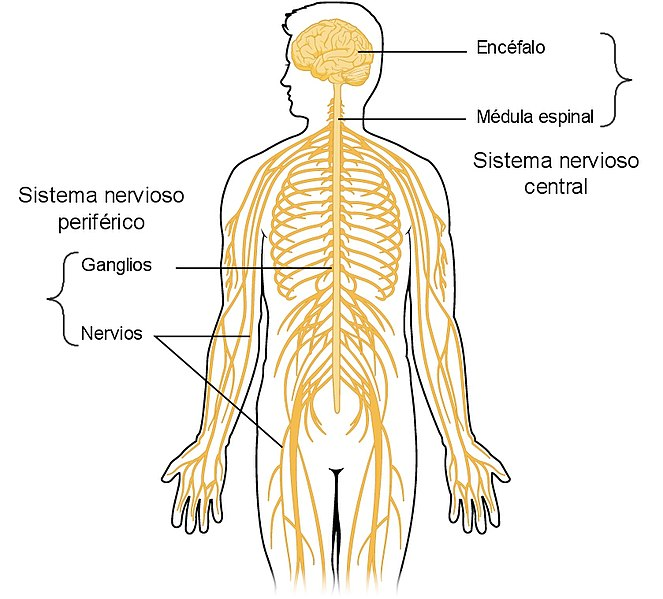
\includegraphics[scale=0.5]{../Figuras/Nervous_System.jpg}
 \caption{Overview of Nervous System esp, OpenStax, 20 diciembre 2018, WIKIMEDIA COMMONS, \url{https://upload.wikimedia.org/wikipedia/commons/0/07/1201_Overview_of_Nervous_System_esp.jpg}, CC BY-SA 4.0}
 \label{fig:SNCySNP}
\end{figure}


En del sistema nervioso periférico tenemos al:


\begin{itemize}
 \item \textbf{Sistema somático} se controla de forma voluntaria, se conforma de nervios conectados a músculos voluntarios esqueléticos y receptores sensoriales, de los cuales unos son:
 \begin{itemize}
  \item de entrada, \textbf{aferentes}
  \item de salida, \textbf{eferentes}
 \end{itemize}


 \begin{figure}[h]
 \centering
 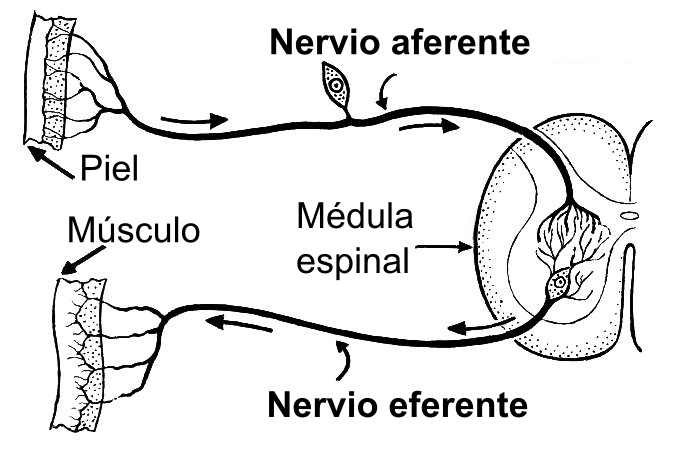
\includegraphics[scale=0.5]{../Figuras/afferent_efferent.png}
 \caption{Diagrama explicativo del recorrido eferente y el aferente, Pearson Scott Foresman, 26 August 2010, WIKIMEDIA COMMONS, \url{https://upload.wikimedia.org/wikipedia/commons/3/3e/Afferent_\%28PSF\%29.es.png}, CC0}
 \label{axonesSA}
 \end{figure} 
 
\item \textbf{Sistema autónomo} funciona de forma involuntaria, se conforma de nervios que se conectan con el corazón, los vasos sanguíneos, los pulmones, el estómago, los intestinos, glándulas
\end{itemize}


Ahora respecto al sistema nervioso central lo integra:


\begin{itemize}
 \item La médula espinal
    \begin{itemize}
     \item Dentro de esta hay una organización, la presencia de \textbf{ciclos de retroalimentación local}, es decir, nuestro sistema va a estar en diferentes etapas son nervios que no necesitan pasar por todo el procesamiento cerebral, las señales simplemente entran llegan a una fase local e inmediatamente reaccionan, ver el ejemplo de la imagen \ref{actReflejo}. Ocurren en un ciclo local y esto también puede convertirse en algo muy importante a la hora de hacer cómputos, no siempre es necesario pasar todo por todas las capas de procesamiento. 


     \begin{figure}[h]
      \centering
      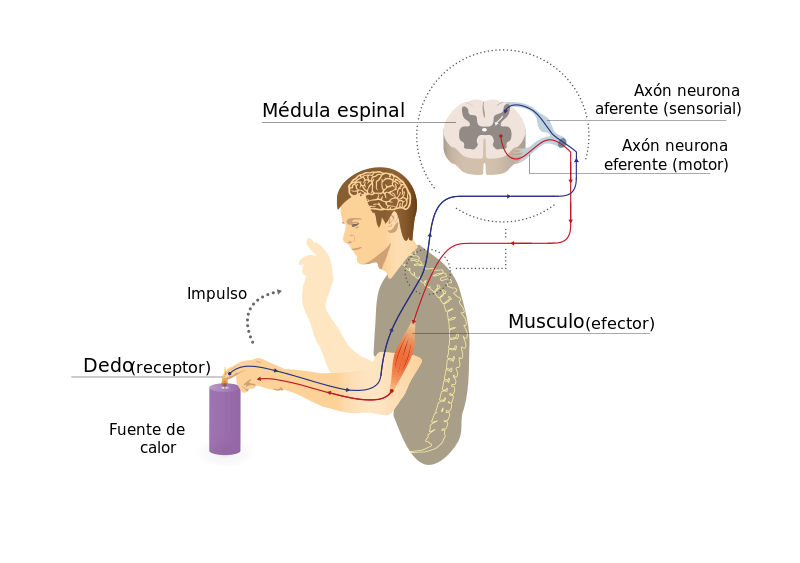
\includegraphics[scale=0.4]{../Figuras/actReflejo.png}
      \caption{ Esquema explicativo del arco reflejo, Marta Aguayo, 18 diciembre 2014, WIKIMEDIA COMMONS, \url{https://upload.wikimedia.org/wikipedia/commons/c/cb/Imgnotraçat_arc_refelx_esp.svg}, CC BY-SA 3.0.}
      \label{actReflejo}
     \end{figure}


     \item \textbf{Señales de control motor descendientes} del cerebro hacia las neuronas motoras, estas son señales que provienen de un campo en una capa mucho más alta de procesamiento y provocan movimientos.
     
     \item \textbf{Axones sensoriales ascendentes} donde el cuerpo de la neurona está afuera y la información va a viajar hacia arriba, desde los músculos, piel y  estas señales viajan hasta el cerebro.  


     \end{itemize}


 \item El encéfalo
\end{itemize}


 Cada colección de nervios que sale de la base del cerebro se asocian con funciones muy específicas (en su mayoría). 
 
 Notas:
 
 \begin{itemize}
  \item Este sistema está hecho en diferentes niveles locales, entradas y salidas  
  \item El procesamiento que esté ocurriendo en el encéfalo puede tener diferentes capas y eso se verá reflejado cuando nosotros definamos arquitecturas para las redes neuronales. 
  \item Las redes neuronales actuales, que han tenido más éxito, se componen de diferentes subunidades o diferentes redes que hacen cosas locales. Es decir esta estructura global que estamos viendo,  se está empezando a reproducir/imitar ya con las neuronas computacionales.


 \end{itemize}




\subsection{Cerebro}


En esta parte vamos a preocuparnos sobre todo por la parte funcional. Haciendo una breve analogía, vamos a hacer una visión general del “hardware”, para ver qué efectos va a tener en el “software”. 
En general la arquitectura de cada cerebro es completamente diferente al cerebro de otras personas. Se ha intentado averiguar qué está haciendo cada región con diferentes estudios por ejemplo,  ver cuánta sangre se está bombeando en diferentes regiones del cerebro dependiendo de los estímulos que se le presentan a una persona, o si alguna persona tiene un padecimiento se tratan de tomar escaneos para ver qué regiones del cerebro están funcionando y cuáles presentan lesiones. A partir de las lesiones, lo que hacen es que una vez que está identificada la actividad que ya no se puede realizar de forma normal, averiguan qué región era responsable de esa actividad, que ahora está dañada.


Gracias a esos estudios, se ha logrado identificar más o menos en manera general, a qué se dedica cada una de las regiones del cerebro. En ocasiones no se puede decir exactamente qué tan vinculadas están (las regiones) o por qué se están activando otras regiones.


Hay partes funcionales que se comparten entre las diferentes regiones y no están ubicadas en un solo lugar. Otras parte importante a mencionar es, el cerebelo que se considera prácticamente vital, cumple con funciones tales como el equilibrio, la coordinación, el control fino de los músculos, de hecho tiene más neuronas que el cerebro y aun así hay niños que nacen y viven sin cerebelo. 




A continuación se mencionan algunas de las diferentes funciones de las regiones, que se han identificado en la imagen \ref{cerebro}: 


 \begin{figure}[h]
  \centering
  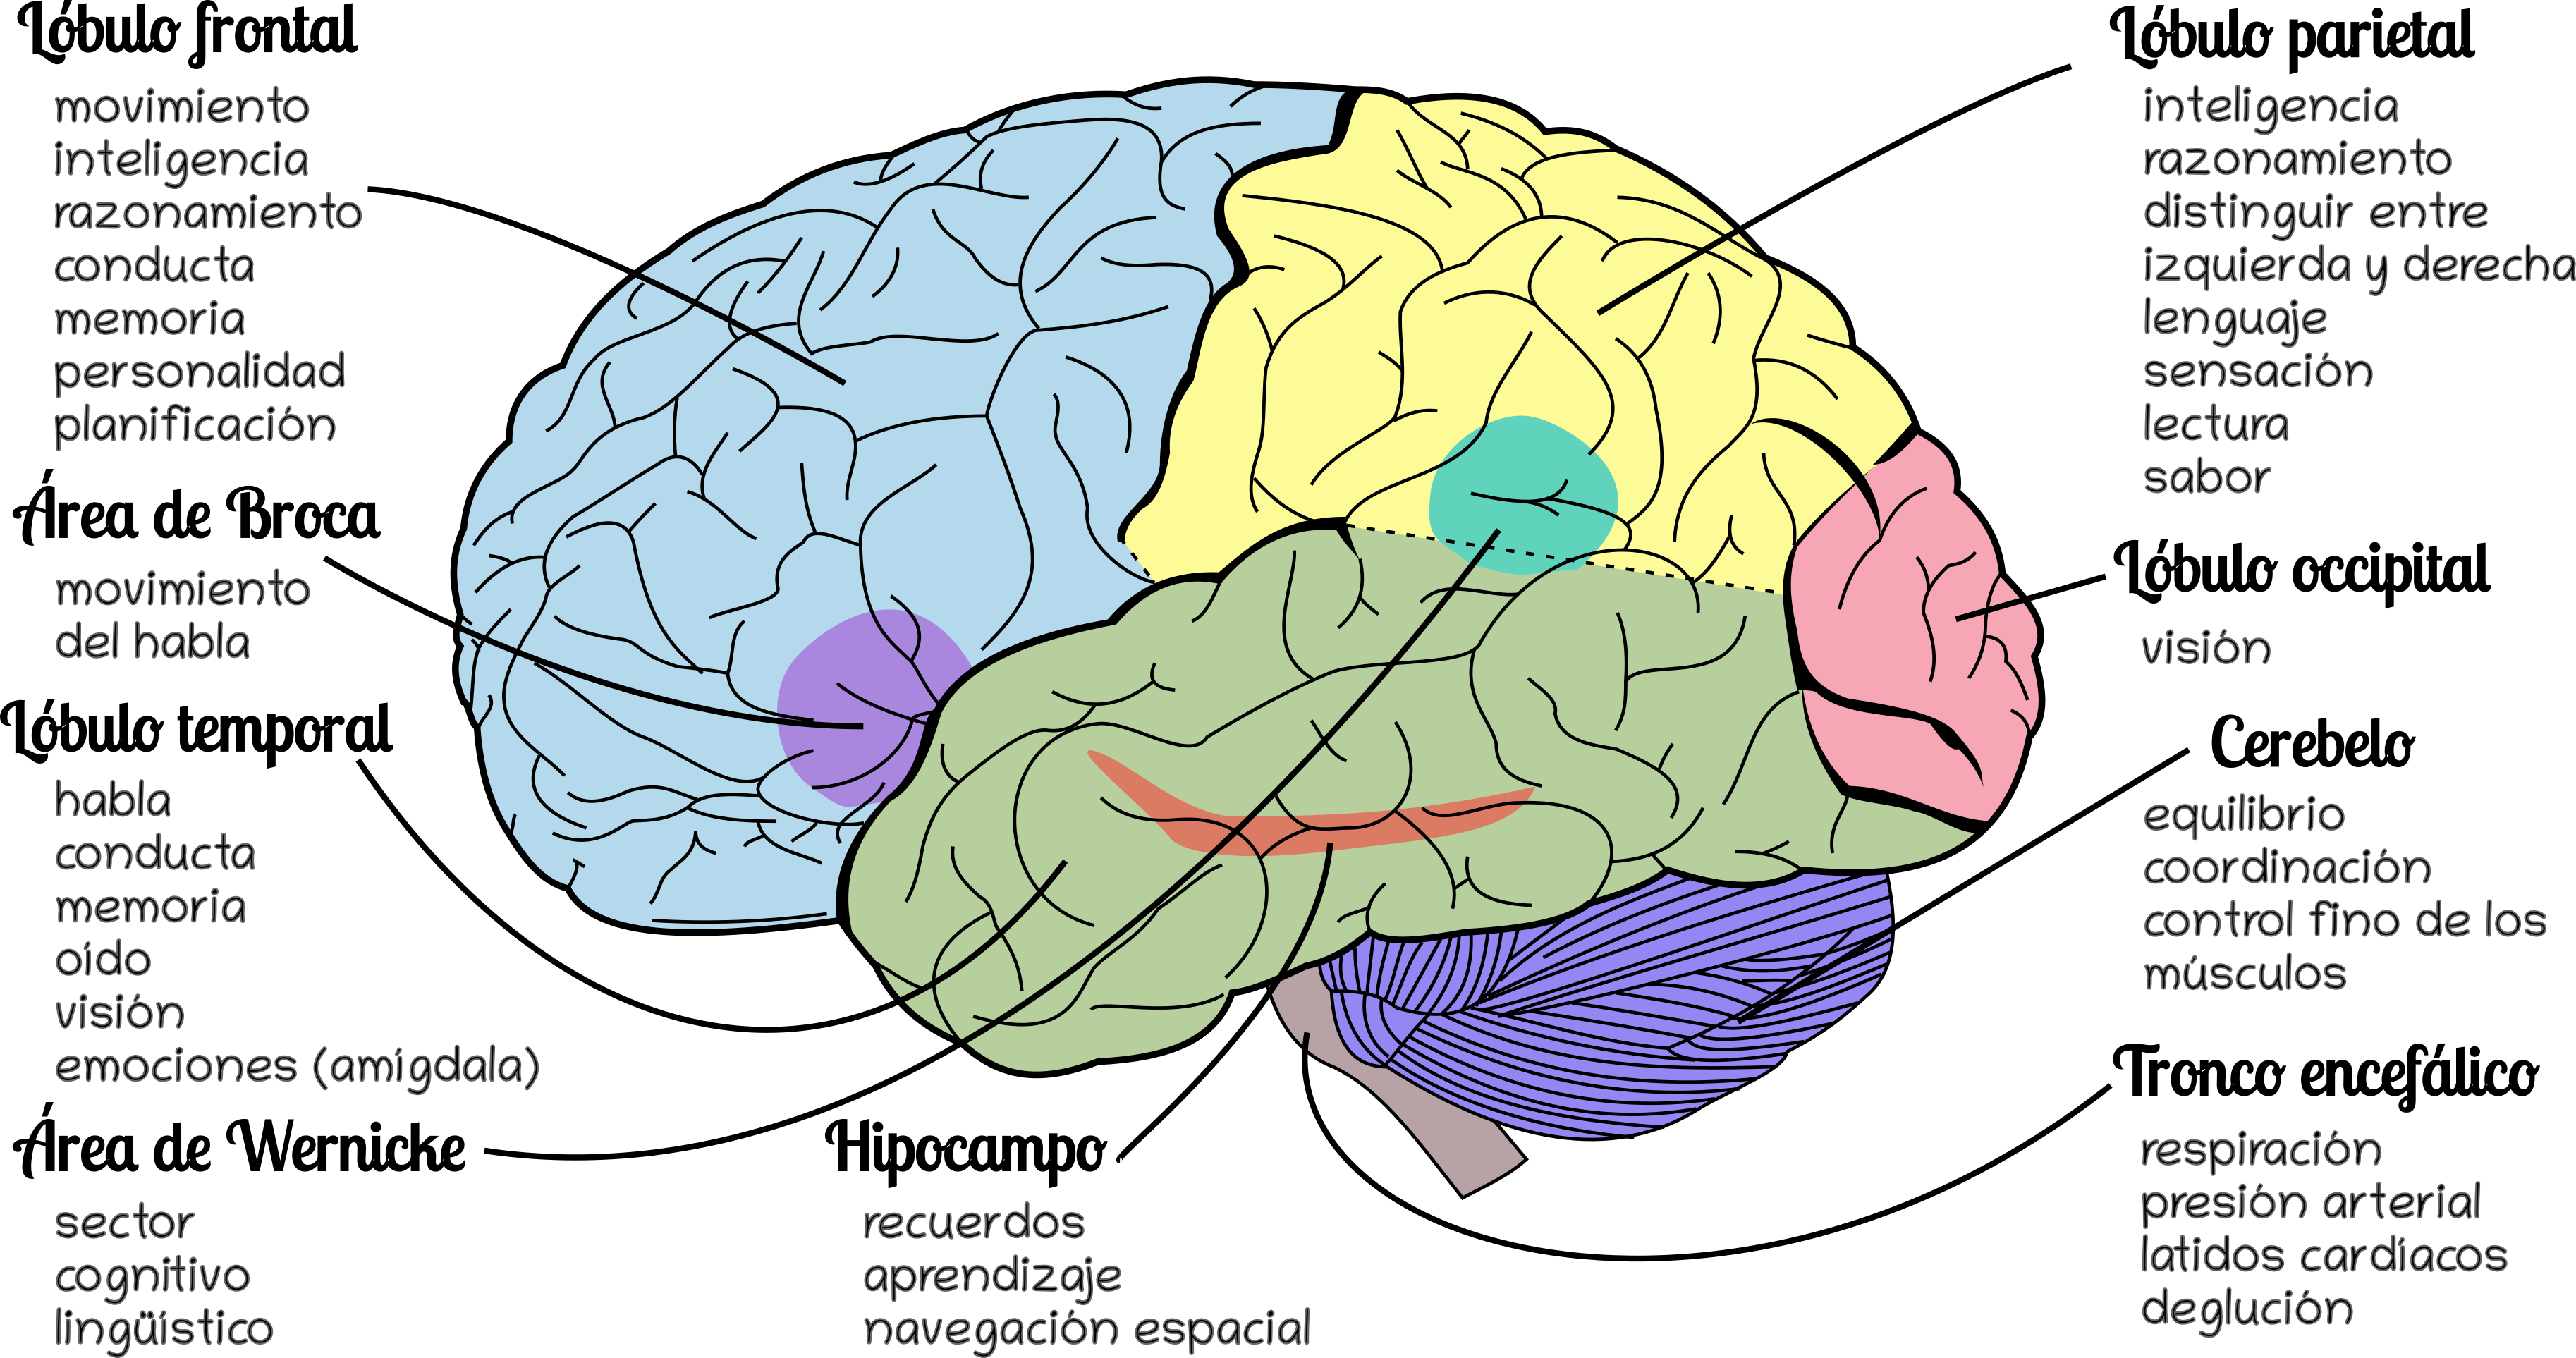
\includegraphics[scale=0.7]{../Figuras/cerebro.png}
  %Presentación Sistema Nervioso
  \caption{Diagrama básico de las regiones del cerebro.}\label{cerebro}
 \end{figure}


\begin{description}
%\begin{itemize}
 \item \textbf{Lóbulo frontal} se le puede asociar con la parte del raciocinio,  la parte de inteligencia, la conducta, la memoria, la personalidad, la capacidad para realizar planes complejos a largo plazo y también es responsable de algunas actividades de movimiento. Dentro de este destaca el área de broca, su principal función es el movimiento del habla, mover los labios, la boca.
 \item \textbf{Lóbulo temporal} aquí está otra parte del habla, que tiene que ver más con el uso de símbolos para el lenguaje, la conducta, memoria, aquí se procesa el oído, un poco de visión y emociones. Dentro de este está (compartida entre el lóbulo parietal) el área de Wernicke, trabaja con la parte lingüística, y de cognición. También dentro de este está el \textbf{hipocampo} trabaja con recuerdos, aprendizaje y navegación espacial, cómo sabemos cómo llegar de un lado hacia otro.
 \item \textbf{Lóbulo parietal} trabaja con la inteligencia, razonamiento, distinguir entre izquierda y derecha, lenguaje, sensación, lectura y sabor. 
 \item \textbf{Lóbulo occipital} se dedica prácticamente solamente a visión, es una región un tanto amplia. En particular en el área de robótica cuando están programando un robot o móvil, los robots tienen dos laptops y una de ellas se dedica prácticamente solo a procesar la visión.
 \item \textbf{Cerebelo} se encarga del equilibrio, la coordinación fina de los músculos.
 \item \textbf{Tronco encefálico} se encarga de la respiración, presión arterial, latidos cardíacos, de ilusión, conciencia. 
%\end{itemize}
\end{description}


\subsection{Zonas funcionales}
Para visualizar mejor la parte de la arquitectura, que tiene el cerebro para realizar todo lo que se le conoce como,  la ruta desde la sensación hasta la cognición, veremos un diagrama de la parte funcional del cerebro.  


 \begin{figure}[h]
  \centering
  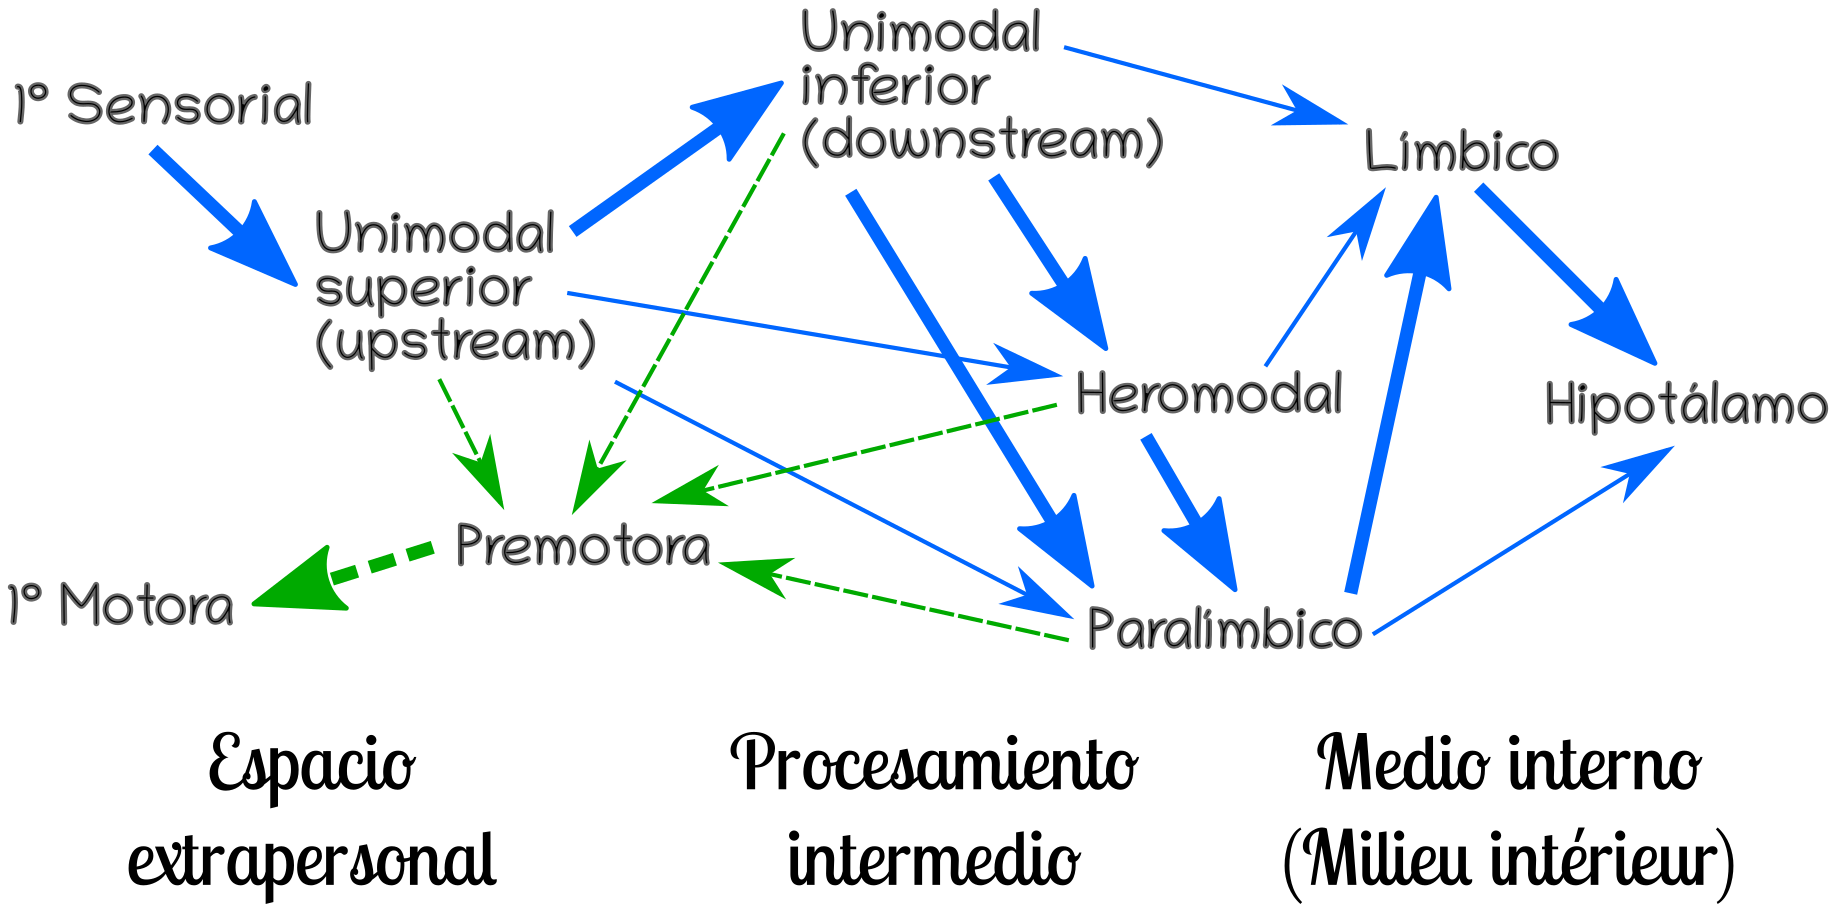
\includegraphics[scale=0.2]{../Figuras/zonasFuncionales.png}
  %Presentación Sistema Nervioso (11)
  \caption{Diagrama de la arquitectura del cerebro a nivel funcional.}
  \label{fig:zonasFun}
 \end{figure}


Explicando el diagrama \ref{fig:zonasFun}, en la primera parte (espacio extrapersonal) vamos a pensar en la entrada sensorial, que se enfoca muchísimo en la parte de visión y audio (en general todos los sentidos), notamos qué de las neuronas que están en la parte sensorial, su primera conexión es hacia una capa que se le llama unimodal superior,  aquí se procesa la información de cada sentido de manera individual, es decir, las neuronas o solamente están procesando visión o solamente audio, todavía no se mezclan, por ejemplo de visión, se separan colores e intensidad lumínica, se empieza a detectar algunas esquinas, alguna inclinación, la dirección de las luces y las sombras. Notemos que desde aquí hay una rápida conexión a la sección premotora y luego hacia la parte motora, recordando la mención de los circuitos locales y de reflejos, aquí prácticamente lo podemos ver (en este pequeño camino).


Pasando de este primer procesamiento básico entramos al siguiente que es el unimodal inferior, (aquí aún se está trabajando con procesamiento de una sola modalidad) visión sigue siendo visión, audio sigue siendo audio, pero ya son procesamientos un poco más complejos, por ejemplo, reconocimiento de rostros, de objetos. En esta parte tenemos un rápido ciclo de regreso a la parte premotora, por ejemplo la acción de ver a mi mamá y saludarla (aquí aún no se tiene que razonar demasiado). 


En la siguiente fase (medio interno), se conecta hacia tres áreas, la \textbf{heromodal}, ya se integran diferentes modalidades (audio y visión) ejemplo, oigo que me hablan y volteo a ver, aquí se está juntando ambas cosas, el \textbf{límbico} y el \textbf{paralímbico} que trabajan con la parte de las emociones y conceptos abstractos.


Finalmente, llegamos al \textbf{hipotálamo} que es donde están todas las emociones, en las conexiones entre estas regiones, estarían los procesamientos de alto nivel.


Ahora estas diferentes regiones se replican de cierta manera cuando estamos haciendo los diseños de las arquitecturas modernas para redes neuronales.
En algunas ocasiones se comienza con algunas capas de neuronas, haciendo procesamientos con una sola modalidad, extrayendo datos básicos, después se van
componiendo en figuras más complejas y después hasta podemos combinar bloques de neuronas, para poder resolver problemas que tomen en cuenta diferentes modelos.






 
\section{Neurona biológica}
\subsection{La neurona}
La neurona es un tipo de célula perteneciente al sistema nervioso central, que se comunica tanto por señales eléctricas como por señales químicas. Cada neurona tiene:


 \begin{itemize}
	\item Un cuerpo celular (\textbf{soma}) que contiene un núcleo y otros componentes celulares.
	\item Una zona de recepción denominada \textbf{dendritas}.
	\item Una zona de emisión conocida como \textbf{axón}, compuesto de:
		\begin {itemize}
			\item Cono axonico.
			\item Membrana plasmática axonica y citoplasma.
			\item Recubrimientos de mielina, interrumpidos con intervalos regulares de nódulos (anillos) de Ranvier.
			\item Terminales del axón donde se encuentan los \textbf{botones sinapticos}. 
		\end{itemize}
 \end{itemize}


\begin{figure}[h]
 \centering
 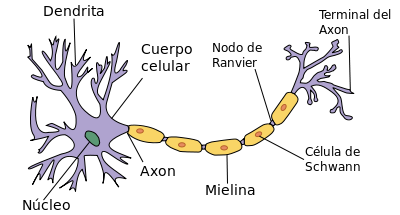
\includegraphics[scale=0.6]{../Figuras/neuronaPartes.png}
 \caption{Neurona, Acracia, 14 January 2007, Wikimedia Commons, \url{https://commons.wikimedia.org/wiki/File:Neurona.svg}, Creative Commons Attribution-ShareAlike 2.5 Generic}
 \label{fig:neuronaP}
\end{figure}


 Pensemos en la neurona como toda una compuerta, por un lado, está el cuerpo de una neurona típica, en las dendritas tenemos una mezcla de neurotransmisores y iones que pueden moverse a través de la membrana. La forma en que intercambia información es mediante sustancias químicas y iones que se están intercambiando, entre la parte de afuera y de adentro de la neurona. Particularmente en las dendritas, se tienen terminaciones que se pueden conectar con otras neuronas y de esta manera permitir el paso de información. 
 
 \begin{itemize}
  \item Neurona presináptica, transmite una señal.
  \item Neurona posináptica, recibe una señal.
 \end{itemize}  
 
En el interior de la neurona hay una cierta carga eléctrica, en el exterior (el líquido de afuera) hay otra carga eléctrica, es decir, hay una \textbf{diferencia de potencial} entre el interior y el exterior de la neurona, por eso se dice que la membrana axónica en sí misma tiene una carga eléctrica. Dado que es porosa, esta membrana  va a estar intercambiando partículas con el exterior, esto va a hacer que la polarización de esta membrana vaya cambiando, si en algún momento la diferencia de potencial neta rebasa un cierto umbral.




\emph{Transmisión de señales y almacenamiento de información:}


\begin{enumerate}
 \item La neurona desde sus dendritas recibe señales de otras neuronas vecinas.
 \item Cada señal se va acumulando en su cuerpo hasta el cono axónico, donde se van a estar sumando la contribución de todos los efectos de cambios de potencial.
 \item En el momento que se rebase un cierto valor umbral, la diferencia de potencial se propaga hasta los botones terminales.
 \item La neurona entra en un período refractario, donde empieza a cambiar el potencial entre el cono axónico y el axón de la neurona.
 \item Se va a transmitir un disparo eléctrico en seguida,
 \item La neurona se va a quedar totalmente quieta, durante un breve momento para que la señal pueda viajar hacia el axón.
 \item Se va a notar un cambio muy violento en el voltaje, que se va recorriendo a lo largo de todo el axón. 
\end{enumerate}


La neurona típica tiene unas células de mielina, que forman nodos que van cubriendo al axón para evitar que se pierda la señal, estos nodos recargan otra vez la señal y permite que avance, al siguiente nodo, donde se recarga  nuevamente y avance, hasta que logre llegar al final de axón.


\begin{figure}[h]
 \centering
 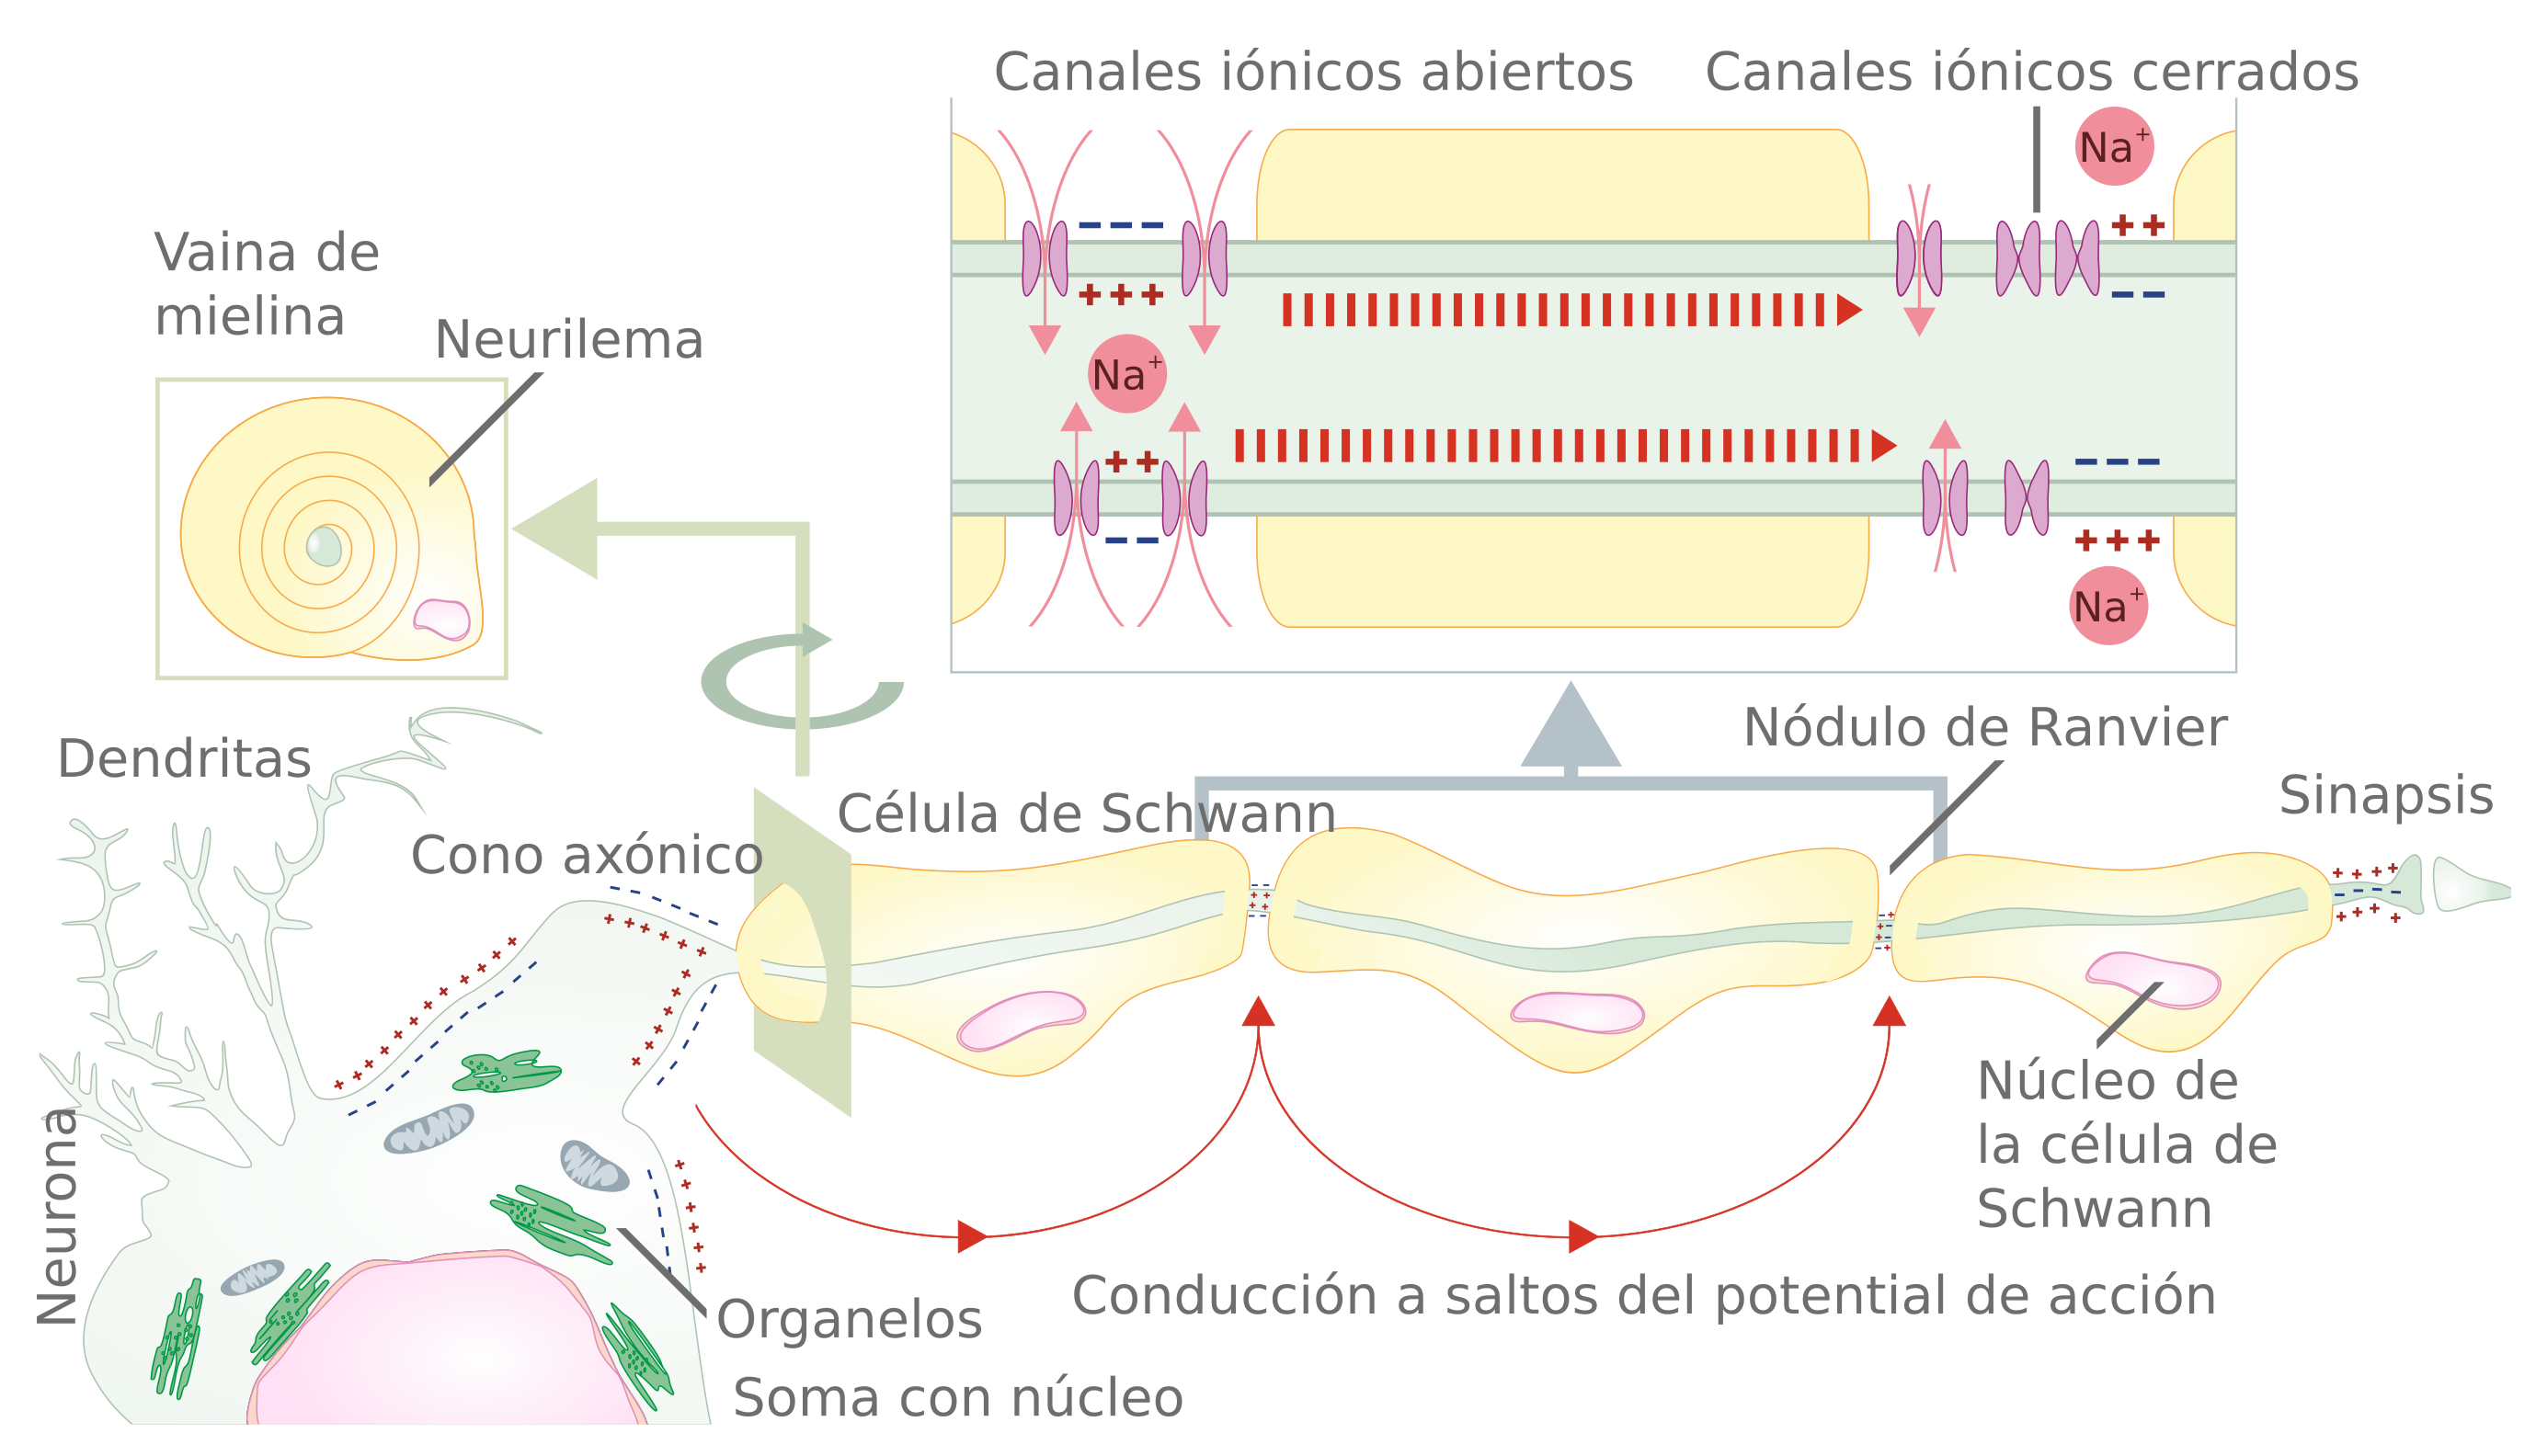
\includegraphics[scale=0.1]{../Figuras/Saltos.png}
 \caption{Corriente iónica por el axón (efecto de corto plazo), Helixitta, 1 octubre 2015, Wikimedia Commons, \url{https://commons.wikimedia.org/wiki/File:Propagation_of_action_potential_along_myelinated_nerve_fiber_en.svg}, Creative Commons Attribution-ShareAlike 4.0 International}
 \label{fig:conduccionSaltos}
\end{figure}


Este trayecto puede ser de una neurona a unas pocas neuronas vecinas, hasta unos cuantos metros (ej. esta podría estar en la médula espinal y el axón llegar hasta el dedo). Cuando la señal llega a la terminal de el axón, hay varias terminales que van a reaccionar ante el cambio de electricidad, mediante la liberación de unas vesículas, que contienen \textbf{neurotransmisores}.




\subsection{Elementos de las neuronas y tipos}


Elementos durante la transmisión de señales:


\begin{itemize}
\item \textbf{Neurotransmisores:} son los mensajeros químicos que se comunican entre neuronas adyacentes; La liberación de neurotransmisores de una neurona ayudará a despolarizar o hiperpolarizar (aumentar la magnitud de la carga) la neurona adyacente, lo que hará que sea más o menos probable que ocurra un potencial de acción en la siguiente neurona.
 
\item \textbf{Impulsos eléctricos:} potenciales de acción que son, cambios de voltaje que van a ir ocurriendo a lo largo del axón. Sucede una vez que se acumularon demasiadas señales a través de las dendritas, entonces la neurona puede disparar un impulso eléctrico, a través del axón, que va a provocar que su terminal libere más químicos, estos químicos son los que hacen los efectos pequeños en cada uno de los cuerpos de las neuronas posinápticas.
 
\item \textbf{Plasticidad:} modificación a largo plazo de las conexiones entre neuronas. En el cerebro las neuronas pueden cambiar de manera permanente, perder canales (que permiten el intercambio de nuevos transmisores sin impulsos eléctricos), formar más canales o incluso pueden crear protuberancias. Por ejemplo, cuando un cerebro aprende está transformando su arquitectura, es decir, los aprendizajes de largo plazo, modifican el cerebro y en consecuencia va a pensar y reaccionar distinto, que antes del aprendizaje.
\end{itemize}

\emph{Clasificación de tipos de neuronas:}




\begin{figure}[h]
 \centering
 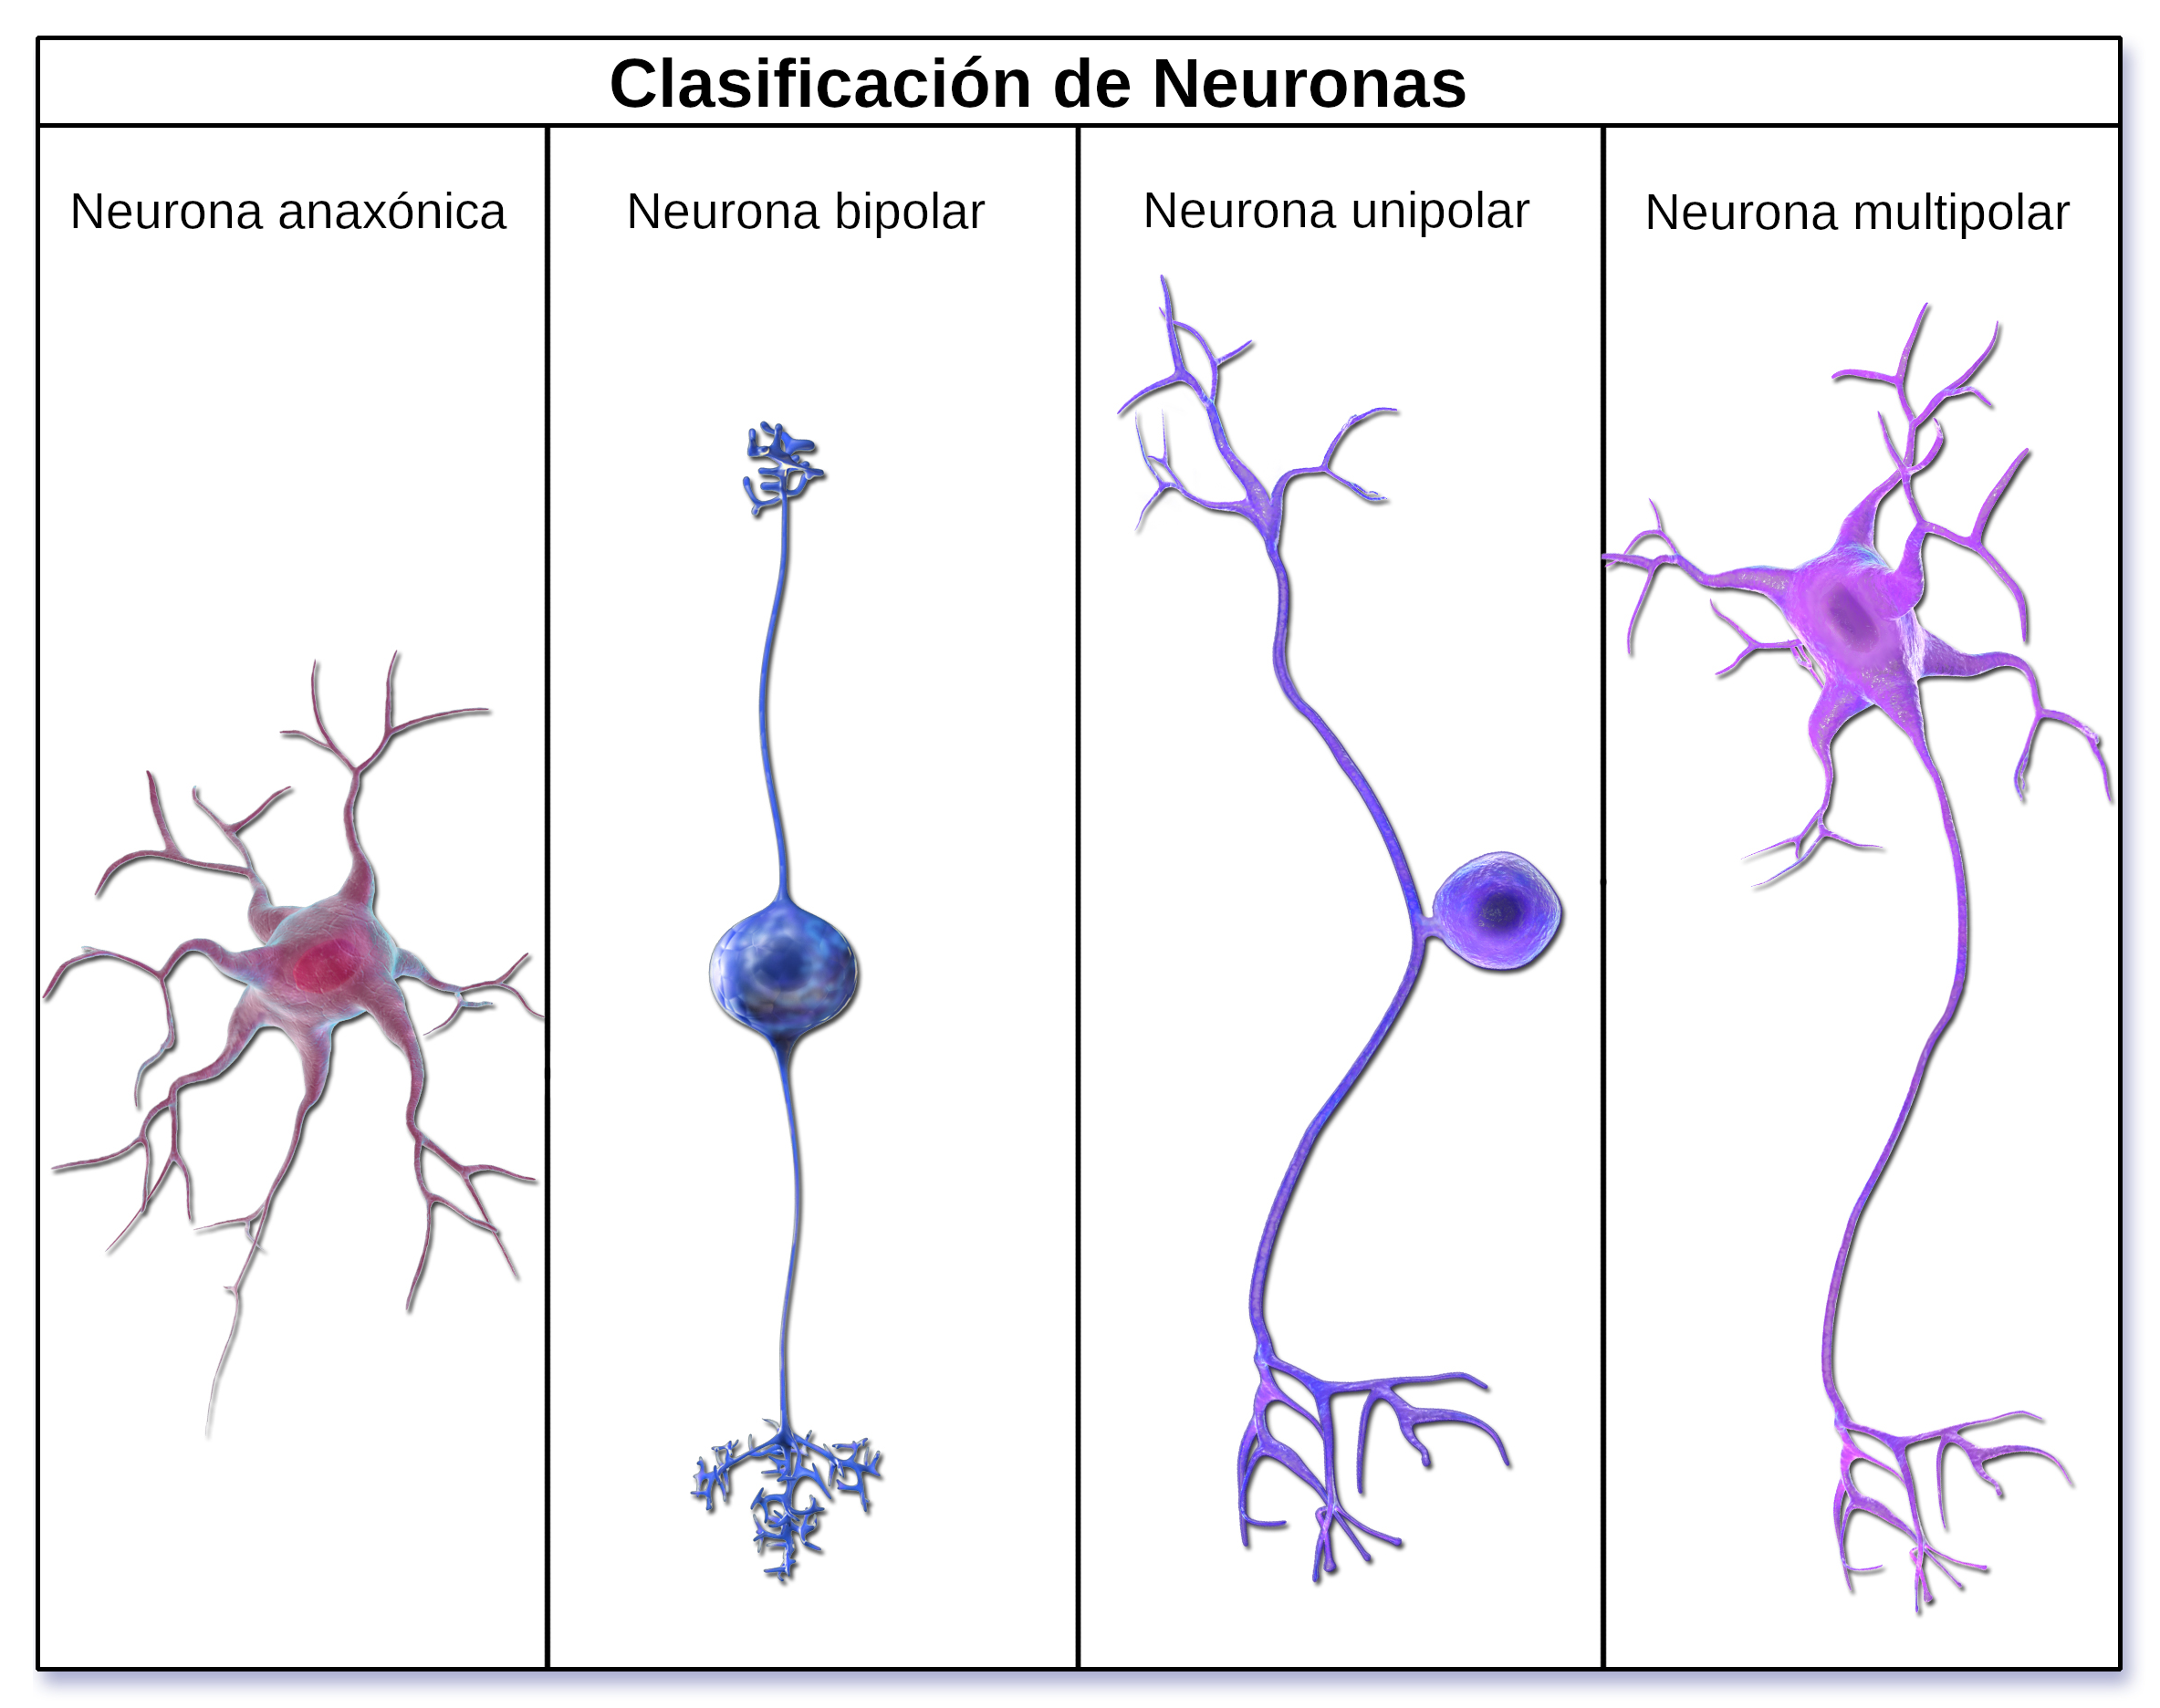
\includegraphics[scale=0.15]{../Figuras/tiposDeNeuronas.png}
 \caption{Representación de la clasificación de neuronas, BruceBlaus, 26 junio 2017, Wikimedia Commons, \url{https://commons.wikimedia.org/wiki/File:Neuron_Classification.png}, Creative Commons Attribution-ShareAlike 4.0 International}
 \label{fig:tiposNeuro}
\end{figure}




\begin{itemize}
\item \textbf{Neuronas sin axones}, nunca dispara, pero si tiene intercambios de neurotransmisores en las dendritas 
\item \textbf{Neuronas bipolares}, tienen dos axones. 
\item \textbf{Neurona unipolar}, solamente hay una conexión entre el cuerpo y el axón, pero el axón tiene dos ramas, cuando dispare va a disparar hacia los dos lados, haciendo llegar su señal a diferentes regiones. 
\item \textbf{Neurona multipolar}, la más conocida, empieza con un cuerpo con dendritas y luego un largo axón que va a terminar con varias terminaciones axónicas. 
\end{itemize}


Cuando modelamos redes neuronales lo típico es modelar, una neurona con dendritas, su disparo y su axón, que se conecta con las siguientes dendritas, pero aquí ya estamos viendo que la naturaleza nos dice que hay que pensar más y plantear cómo hacer las representaciones de estas conexiones que nos presenta la naturaleza, un poco diferente pero tal vez con resultados más satisfactorios.




\subsection{Sinapsis}


Aquí veremos más a detalle cómo una neurona recibe o transmite información a otras neuronas, donde para un solo disparo están participando un montón de elementos que veremos más adelante.


 El momento en que dos neuronas transmiten información se llama \textbf{sinapsis} y es mediante conexiones que se dan en las terminales del axón (vesículas sinápticas) de la neurona presináptica hacia la postsináptica. Es importante notar que estas neuronas no tienen contacto anatómico, sino que están separadas por un espacio muy pequeño, \textbf{la brecha sináptica}. Lo que sucede en estas conexiones es un intercambio electroquímico que produce cambios de polaridad a lo largo la membrana. 




\begin{figure}[h]
 \centering
 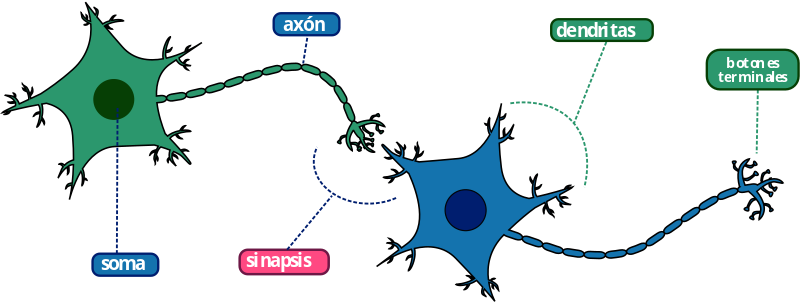
\includegraphics[scale=0.5]{../Figuras/Part_of_neurons_in_Spanish.png}
 \caption{Part of neurons in Spanish, Dana Scarinci Zabaleta, 24 febrero 2019, Wikimedia Commons, \url{https://commons.wikimedia.org/wiki/File:Part_of_neurons_in_Spanish.svg}, OpenStax, CC0}
 \label{fig:sinapsisN}
\end{figure}


Clasificación de sinapsis, las terminales del axón de la neurona presináptica puede hacer contacto con la neurona postsináptica en:
\begin{enumerate}
 \item su dendritas, axodendrítica.
 \item su cuerpo (soma), axosomática. 
 \item su axón, axoaxónica.
\end{enumerate}


Distingamos entre dos tipos de sinapsis:


 \textbf{Sinapsis eléctrica:} las membranas de las células pre y posinápticas se unen en la brecha sináptica por una unión tipo gap, o unión comunicante, que son pequeños canales que permiten el paso de iones.


	\begin{enumerate}
  	 \item Posee una transmisión bidireccional de los potenciales de acción.
  	 \item Sincronización en la actividad neuronal, lo cual hace posible una acción coordinada.
 	 \item Los potenciales de acción pasan a través del canal proteico directamente sin necesidad de la liberación de los neurotransmisores, por tanto, es más rápida.
	\end{enumerate}


\begin{figure}[h]
 \centering
 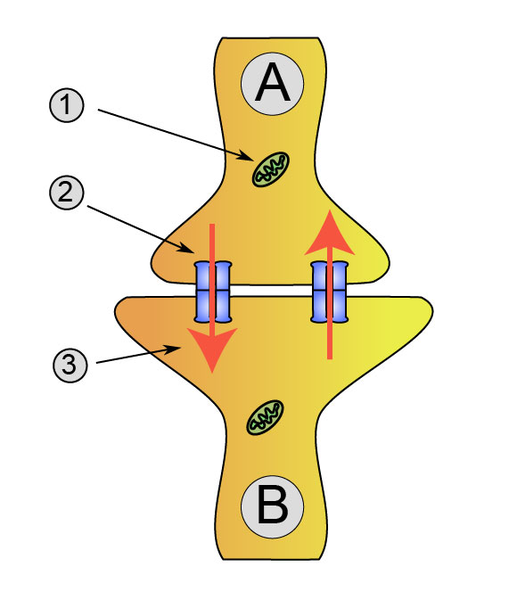
\includegraphics[scale=0.4]{../Figuras/sinapsisElectrica.png}
 \caption{Synaptical transmission (electrical). Neurona A transmisora, Neurona B receptora, 1. Mitocondria, 2. Uniones gap formadas por conexinas, 3. Señal eléctrica, Nrets~commonswiki, 23 September 2005, Wikimedia Commons, \url{https://commons.wikimedia.org/wiki/File:Synapse_diag2.png}, Inkscape 0.42, CC-BY-SA 3.0}
 \label{fig:sinapsisN}
\end{figure}
 
 \textbf{Sinapsis química:} la neurona libera moléculas neurotransmisoras a otra neurona adyacente en un pequeño espacio (la brecha sináptica) ver \ref{fig:sinapsisQ}. Se puede resumir en cuatro etapas principales:


\begin{enumerate}
 \item Un potencial de acción llega al botón terminal proveniente desde cono axónico.
 \item Los neurotransmisores contenidos en las vesículas que están él los botones terminales, son liberados en la brecha sináptica y se dispersan.
 \item Cada neurotransmisor se une a su receptor ubicado en la membrana de la neurona postsináptica.
 \item El exceso de neurotransmisores que queda en el espacio sináptico es degradado o recaptado.
\end{enumerate}


\begin{figure}[h]
 \centering
 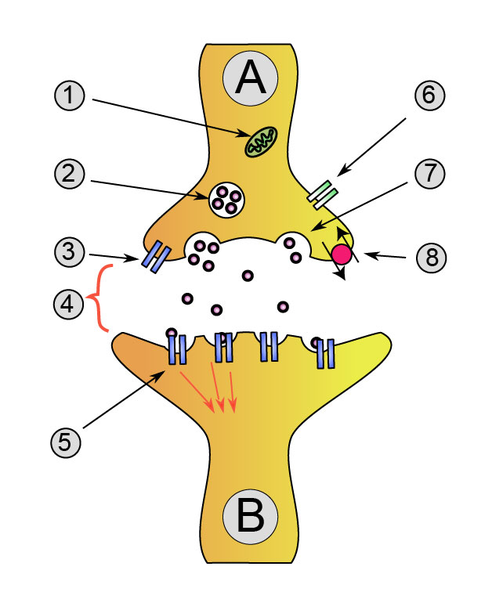
\includegraphics[scale=0.4]{../Figuras/SinapsisQuimica1.png}
 \caption{Synaptical transmission (chemical). Neurona A transmisora, Neurona B receptora, 1. Mitocondria, 2. Vesícula sináptica llena de neurotransmisor, 3. Autorreceptor, 4. Brecha sináptica, 5. Receptor de neurotransmisores, 6. Canal de calcio, 7. Neurotransmisor liberador de vesículas fusionadas, 8. Bomba de recaptación de neurotransmisores, Utilisateur:Dake, 23 September 2005, Wikimedia Commons, \url{https://commons.wikimedia.org/wiki/File:Synapse_diag1.png}, Inkscape 0.42, CC-BY-SA 3.0}
 \label{fig:sinapsisQ}
\end{figure}




Detallando el proceso de la sinapsis química, la neurona postsináptica está recibiendo un montón de señales por la liberación de neurotransmisores tanto de sus vecinos, como lo que ella misma va intercambiando, una vez que están generando el efecto completo de cambiar la polarización de la membrana, van a provocar que la neurona haga un disparo eléctrico. En el cuerpo están llegando estos intercambios de iones que se suman en el cono axónico, empiezan a viajar a través del axón, en las vainas de mielina (donde se refuerza la señal). 
Aquí hacemos mención por primera vez de los iones positivos: sodio y potasio, estos iones lo que hacen es, que \emph{la membrana tenga una cierta carga la mayor parte del tiempo}. Cuando salen tres sodios entran dos potasios, entonces siempre hay más positivos afuera que en el interior de la neurona, es decir, por lo general  \emph{tiene una carga más negativa que su entorno} (ver \ref{fig:MembranaP}). Cuando ocurre un disparo de la neurona y se da el cambio de polarización en la membrana, se abren sus poros/ canales. El hecho que los canales abran o cierren depende de varios cambios que puedan estar ocurriendo alrededor de la neurona, en particular los que transmiten el disparo eléctrico, reaccionan ante el cambio de potencial que ocurrió en la membrana de la neurona. 


La señal va pasando por los nodos de Rainvier, se refuerza y pasa por los canales iónicos ya abiertos, hasta finalmente llegar a la sinapsis a esto le llaman la \textbf{conducción a saltos} (ver \ref{fig:conduccionSaltos}). Ahora lo que ocurre al final del recorrido es que, el cambio de electricidad otra vez provoca que unas vesículas, que están en el interior de la neurona, que contienen neurotransmisores, se peguen a la membrana axónica y se liberen esos neurotransmisores nuevamente a otra neurona. 


Entonces la información le va a llegar a la neurona vecina, en la forma de neurotransmisores que fueron liberados (en lo que sea que lo haya recibido, típicamente son dendritas, pero podría ser su cuerpo o su axón), eso es lo que va a percibir la otra neurona y otra vez esta otra neurona va a empezar a sumar los efectos de estos neurotransmisores, para que en algún momento decida a lo mejor disparar y otra vez provocar que se liberen neurotransmisores a su final e influir con otras neuronas.


\subsubsection{Neurotransmisón}
Cuando la neurona no está mandando señales eléctricas, tiene un potencial de reposo, su diferencia de potencial entre el interior y el exterior de la neurona, es más negativo en el interior y más positivo (o menos negativo) en el exterior.
En el caso de las sinapsis químicas, llega un disparo y se altera el potencial de la membrana, entrarán las
células de calcio y entra la participación de las vesículas para liberar neurotransmisores. Los neurotransmisores están flotando en la brecha sináptica, viajan hasta adherirse a los receptores de la neurona posináptica, en ese momento están alterando el intercambio normal que existe entre \underline{iones en el interior y en el exterior} de la célula y van a cambiar las cargas netas que hay adentro y afuera. Este es un cambio local que está ocurriendo en las  espinas dendríticas (pequeñas prolongaciones citoplasmáticas).


\begin{figure}[h]
 \centering
 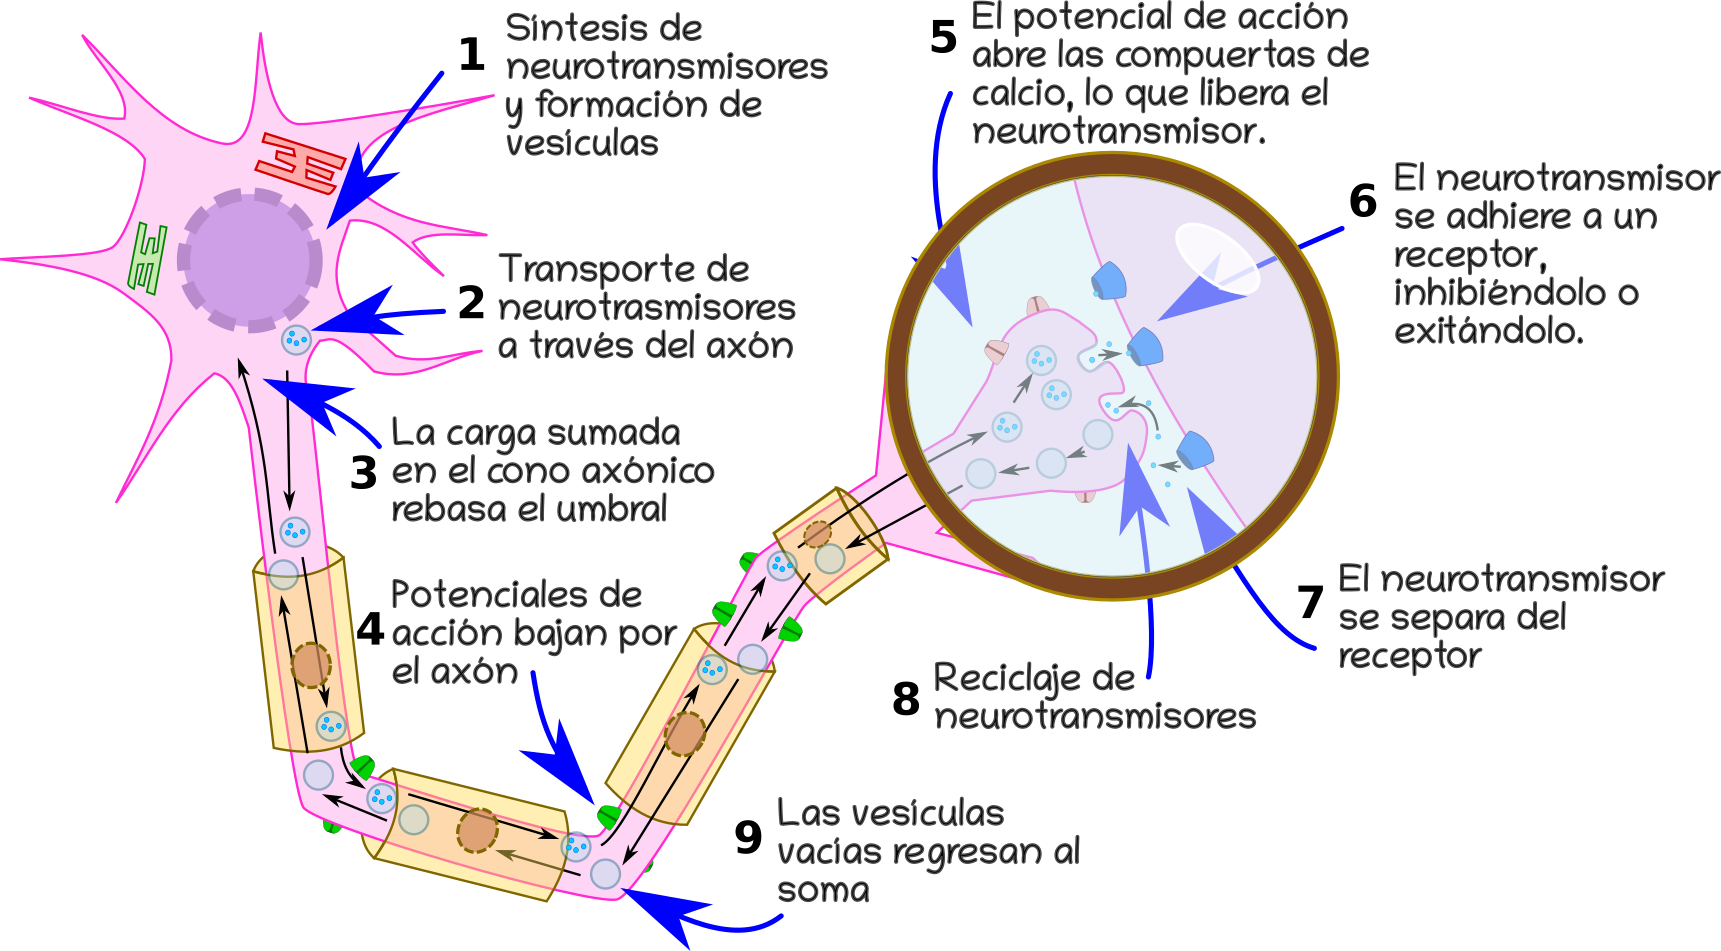
\includegraphics[scale=0.2]{../Figuras/neurotransmision.png} 
 \caption{Esquema detallado de una neurotransmisión.}
 \label{fig:nTransmision}
\end{figure}


este cambio en sí es una especie de transferencia de información, pero muy local.Se puede distinguir entre dos efectos en la membrana: 


\begin{itemize}
\item \textbf{El efecto excitatorio}, despolariza la membrana postsináptica es decir ahora va a ser más propensa a disparar porque ya le cambió la diferencia de potencial que tenía.  
\item \textbf{El efecto inhibitorio}, hiperpolariza la membrana postsináptica, es decir, va a incrementar la diferencia de potencial entre el exterior e interior, pero de tal manera que ahora ya no va a querer disparar esta neurona.
\end{itemize}


De estos efectos también va a darse el efecto de la \textbf{plasticidad}, que es cuando dos neuronas tienden a excitarse juntas, después de esta conexión se va a tender fortalecer, sí más bien tienden a inhibirse lo que va a suceder después es que estos canales empiezan a encoger, haciendo que se reduzcan y ya no dispare.


Ejemplos de neurotransmisores: serotonina, dopamina, oxitocina, endorfinas, adrenalina.




\subsection{Campos receptivos}
Aquí lo que nos interesa es, en qué región puede ser afectada una neurona. Se define un campo receptivo, como la región en la periferia sensorial
dentro de la cual los estímulos pueden, influir la actividad de las células sensoriales (ver \ref{fig:camposR}). Hay diferentes niveles donde pueden aparecer los campos receptivos tanto cerca de la piel, cerca del gusto, el olfato, donde las neuronas van a estar asociadas con otras células que les pueden ayudar, que son sensitivas a los cambios correspondientes, a veces la misma neurona va a tener alguna protuberancia especializada.
También podemos encontrarlos más hacia adentro del nivel de procesamiento, no necesariamente todos van a estar pegados a la parte sensorial física. 
\begin{figure}[h]
 \centering
 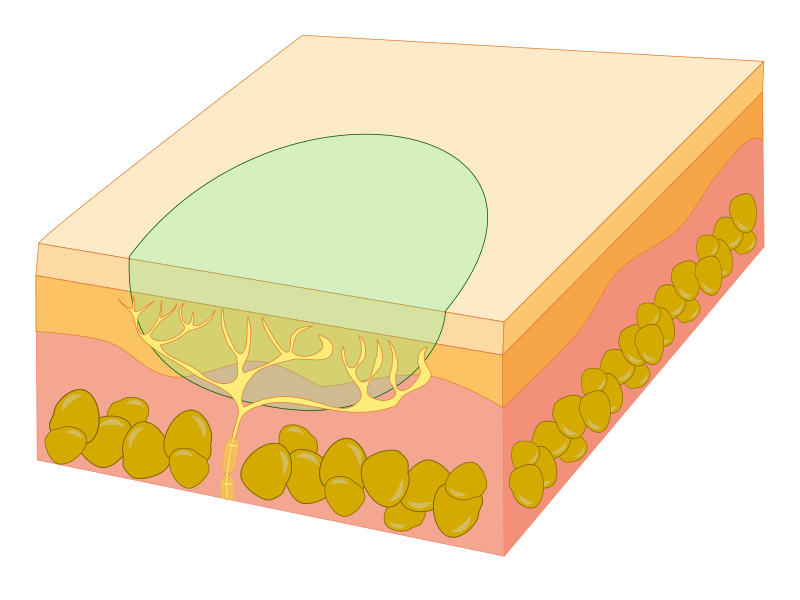
\includegraphics[scale=0.3]{../Figuras/camposreceptores.png}
 \caption{Campo receptivo. Se muestra una región que está bajo cierto estímulo, las terminales de la neurona está recibiendo está información y transmitiéndola.}
 \label{fig:camposR}
\end{figure}


Comprenden a los receptores sensoriales que alimentan a las neuronas sensoriales, pueden ser:


\begin{itemize}
\item Receptores específicos en una neurona como protuberancias especializadas. 
\item Conjuntos de receptores capaces de activar una neurona mediante conexiones sinápticas. 
\item Describen la ubicación donde debe estar presente un estímulo sensorial para licitar una respuesta desde una célula sensorial. 
\end{itemize}


Ejemplos:


\begin{itemize}
\item En la piel tenemos células que nos están protegiendo en la epidermis, una de las células auxiliares \textbf{la célula de Merkel} que es
sensible a la presión. Esta puede estar muy cerca a una neurona, sus terminales se activan de acuerdo a las acciones de la célula de Merkel y va a pasar la información (ver \ref{fig:mer}).  
 	
\begin{figure}[h]
 \centering
 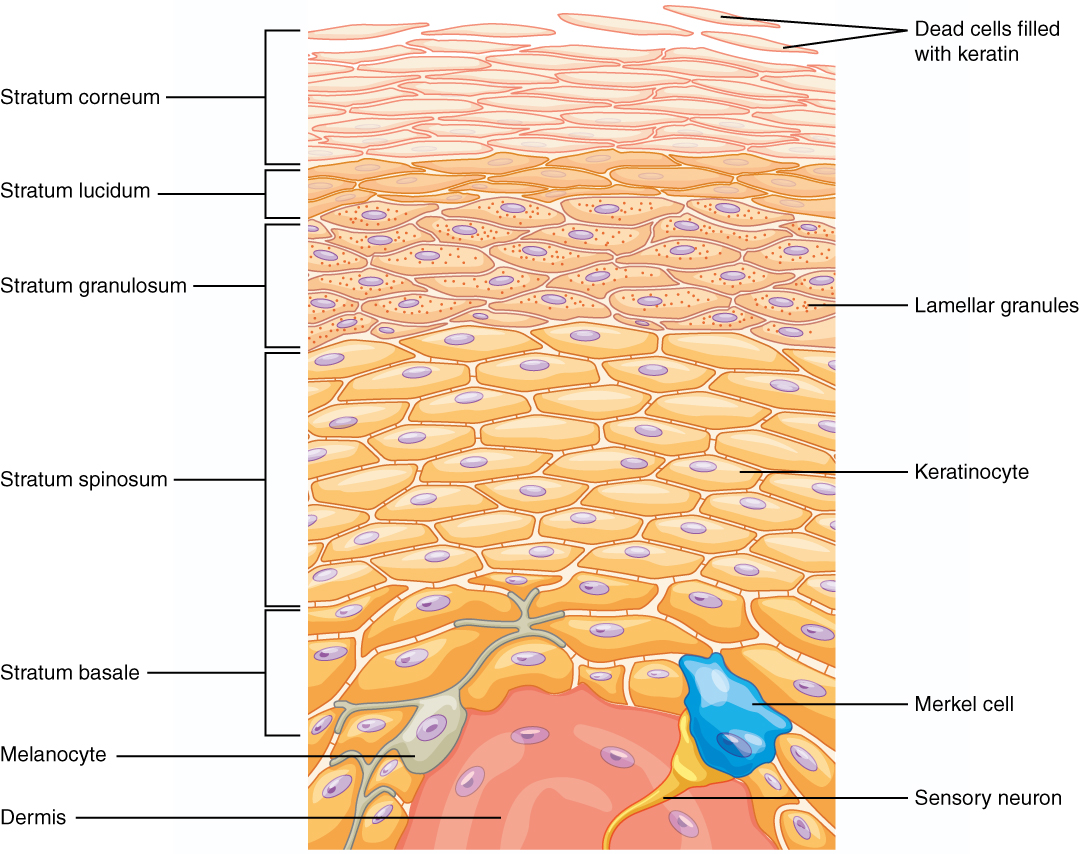
\includegraphics[scale=0.2]{../Figuras/merkel.png}
 \caption{Capas de la epidermis y en azul la célula de Merkel.}
 \label{fig:mer}
\end{figure}


\item El ojo, para procesamiento visual, actualmente se utiliza una de las redes neuronales más famosas que son las redes convolucionales, que están inspiradas en el ojo, nosotros tenemos campos receptores donde hay unos fotorreceptores en los conos y los bastones que son sensibles a luces de diferentes colores a cambios de intensidad de la luz y que pueden detectar, por ejemplo, en una cierta región física si está llegando luz  o por ejemplo, si llega en la periferia entonces va a inhibir el disparo de estos elementos, por otro lado, tenemos también su complemento que permite ser estimulado por las señales que llegan, como que en la parte de afuera de un círculo y más bien se inhiben con un estímulo en la parte de afuera (ver \ref{fig:nSen}). Esta especie de celdas que tienen una posición física y geométrica relevante van a determinar cuando disparan o no las neuronas. Los siguientes niveles del cerebro se van a encargar de interpretar mejor  el cambio de sombras, como a una persona que pasó corriendo, un auto que se está moviendo cerca o reconocer algún tipo de alimento.
\end{itemize}


\begin{figure}[h]
 \centering
 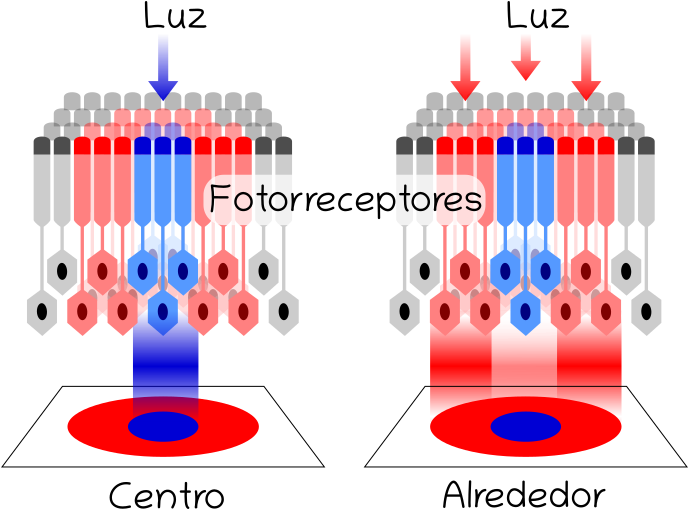
\includegraphics[scale=0.5]{../Figuras/nSensitivas.png}
 \caption{Capas de la epidermis y en azul la célula de Merkel.}
 \label{fig:nSen}
\end{figure}




\subsection{Señal eléctrica}
Veamos que pasa en los canales de iones y el paso de la señal eléctrica primero diferenciemos los tipos de compuertas iónicas:


\begin{itemize}
\item \textbf{Canal por fuga:} Estos se abren y cierran aleatoriamente, todo el tiempo están activos en la neurona, intercambiando por ejemplo: sodio y potasio.
\item \textbf{Canal regulado por ligado:} Aquí se hace presente un neurotransmisor que es el que va a provocar que se abran o al revés impedir que se abran.
\item  \textbf{Canal por estímulo mecánico:} Permiten que pasen más iones o menos iones dependiendo, si se ejerció una presión, por ejemplo, con las neuronas cerca
de la piel, las células de merkel.
\item \textbf{Canales regulados por el voltaje:} Tienen el rol protagónico en la transmisión del pulso eléctrico (que se ha estado mencionando) describiendo uno de ellos, este canal tiene una pequeña compuerta abajo, que la puede cerrar independientemente del hecho de que el canal se abre o se cierre. Existen varias variantes de este tipo de canales regulados por el voltaje, la forma en que se están activando y desactivando sus compuertas, es lo que permite el paso del pulso.
\end{itemize}


Existen realmente una buena cantidad de iones presentes en el cerebro, pero los más protagónicos son precisamente el \textbf{potasio}, el \textbf{sodio}, el \textbf{cloro} y son los que vamos a utilizar para un modelo matemático de las neuronas. 


\begin{figure}[h]
 \centering
 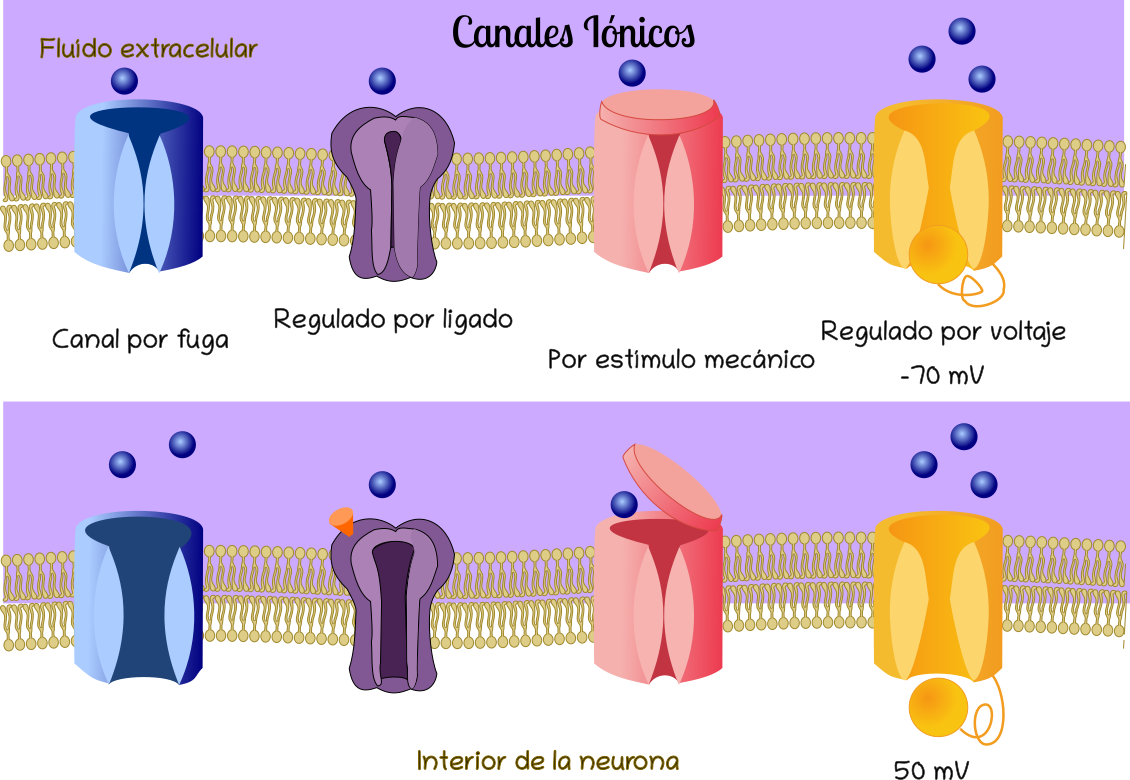
\includegraphics[scale=0.28]{../Figuras/canalesIonicos.png}
 \caption{Representación de la clasificación de los canales iónicos (más representativos).}
 \label{fig:MembranaP}
\end{figure}




Por último veamos brevemente \textbf{la neuroplasticidad}, es lo que nos permite el aprendizaje a largo plazo en el cerebro, es un mecanismo de aprendizaje del cerebro en el cual:


Cuando las neuronas se activan simultáneamente con frecuencia la conexión entre ellas se fortalece.


Este mecanismo constituye la principal inspiración para el diseño de las redes neuronales artificiales, concretamente en esto se inspiran los algoritmos de entrenamiento. Lo que se hace es calcular, qué conexiones debemos reforzar y cuáles debemos de debilitar para que nuestras redes neuronales calculen las funciones que a nosotros nos interesan.


\begin{figure}[h]
 \centering
 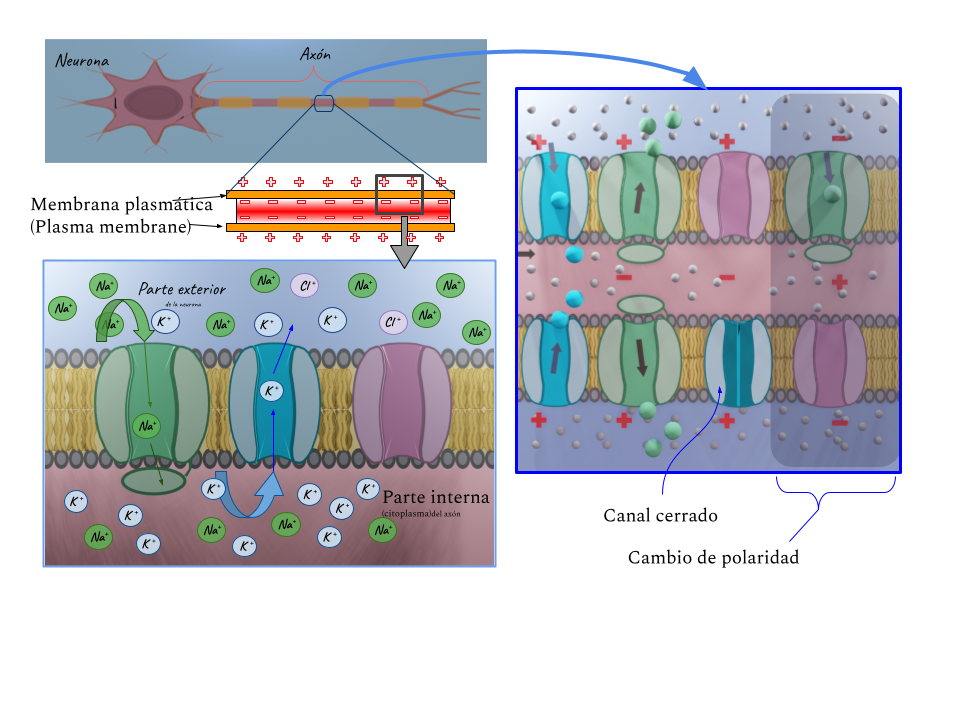
\includegraphics[scale=0.5]{../Figuras/MembranaP.png}
 \caption{Representación de la membrana axónica en potencial de reposo en la parte infererior izquierda, y en la parte derecha con un estímulo que genera el cambio de polaridad en la misma, así como el cierre de canales y paso de iones.}
 \label{fig:MembranaP}
\end{figure}




\chapter{Modelo de Hodgkin-Huxley}

\section{Introducción}

Esta sección se enfocará a la parte de transmisión de información y tipo de operaciones lógicas matemáticas que ocurren para que un cerebro pueda realizar cómputos. Específicamente se detallará la mecánica de los disparos de las neuronas, siendo estos una de las características más relevantes a la hora de modelar las redes neuronales artificiales. Si en algún momento de su vida han visto temas relacionados con: compuertas digitales, arquitectura de computadoras o diseño electrónico digital, les será más fácil abstraer el concepto, pues vamos a ver los procesos de paso de información a través de compuertas pero en un sistema biológico (de la naturaleza). 

Notemos primeramente un impulso nervioso, recordemos que esté es una onda que avanza desde el cono axónico de la neurona hasta la neurona postsináptica. Esta onda electroquímica ocurre dada la diferencia de potencial entre la parte interna y externa de neurona, está diferencia se da a consecuencia de las distintas concentraciones de iones en ambos lados de la membrana plasmática. Los estados en la membrana plasmática (del axón) se pueden diferenciar en, potenciales neuronales:

\begin{itemize}
\item \textbf{Potencial de reposo:} Es la diferencia de cargas en la membrana y está polarizada a -70 mV. Es positiva por fuera (Na+) y negativa por dentro por Cl- y proteínas- y no transmite señal. 
\item \textbf{Potencial de acción o membrana:} Un estímulo umbral de 55 mV, despolariza la membrana y abre los canales del Na+ y K+ y avanza la señal nerviosa, es un cambio muy rápido en la polaridad de la membrana de negativo a positivo y vuelta a negativo.
\end{itemize}

%(Insertar esquema) 
\begin{figure}[h]
 \centering
 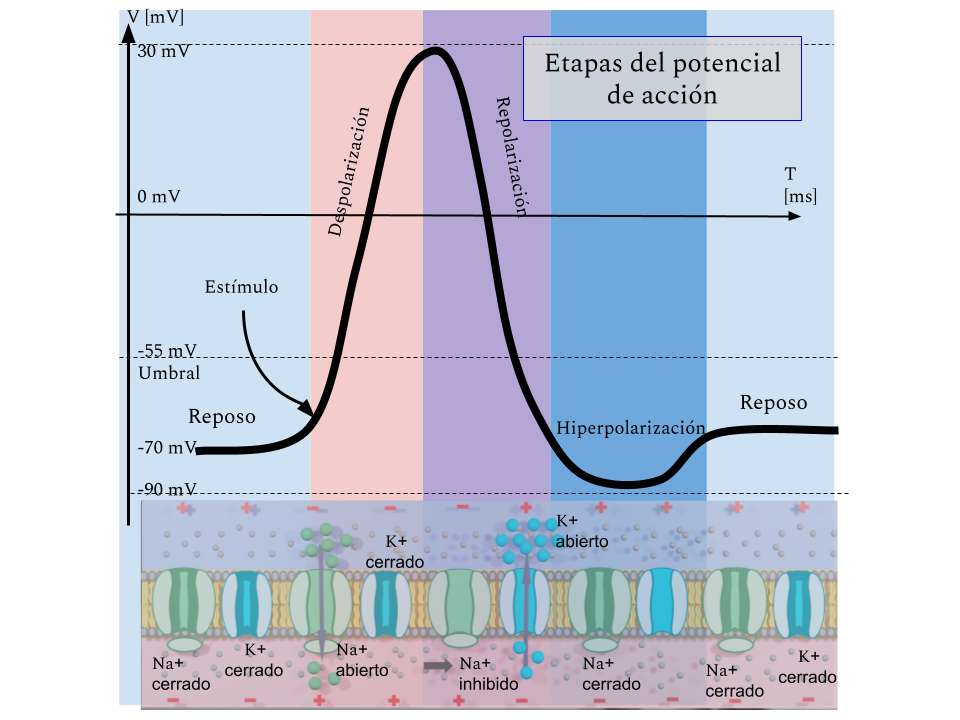
\includegraphics[scale=0.5]{../Figuras/Grafica.png}
 \caption{Representación gráfica de la respuesta de los canales iónicos de sodio (Na+ en verde) y potasio (K+ en azul) ante un estímulo de voltaje, dando como resultado un potencial de acción que viajará a lo largo de todo el axón.}
 \label{fig:graficaP}
\end{figure}

Retomando la sinapsis eléctrica, donde participan los canales iónicos y las entradas de las neuronas (dendritas) están siendo alteradas poco a poco, hasta que ocurre la suficiente carga (diferencia de potencial) en sus dendritas y en el cuerpo de la neurona, para que desde el cono axónico sé dé un disparo o potencial de acción (spike), transmitiendo la información gracias a la apertura y cierre de ciertos canales de iones cargados. Este cambio brusco de la diferencia de potencial, se nota en forma de un pulso eléctrico (ver \ref{fig:graficaP}), para saber más a detalle qué está ocurriendo en esta rápida elevación en la diferencia de potencial, se contará de dónde salió este modelo y por qué toma la forma que tiene. 

Los primeros científicos que estudiaron el potencial de acción y dieron un modelo (de la unión sináptica eléctrica) fueron Alan Lloyd Hodgkin y Andrew Fielding Huxley alrededor de 1952, obteniendo un modelo matemático \footnote{El texto original de este experimento se puede encontrar en la siguiente url: \url{ https://physoc.onlinelibrary.wiley.com/doi/pdf/10.1113/jphysiol.1952.sp004764}}, que intenta explicar qué es lo que estaba pasando en las neuronas. Ellos trabajaron con un calamar gigante (que puede medir hasta 4 metros de largo) que dado su gran tamaño, tiene un axón también bastante gigantesco, que recorre casi la mitad del cuerpo del calamar y su grosor es de medio milímetro, considerando el tamaño estándar de un axón de una neurona (1-20 µm). El axón del calamar gigante es tan grande que les permitió introducir dispositivos para medir el voltaje, es decir, la diferencia de potencial entre, el interior de la neurona y la parte de afuera (el ambiente externo de la neurona). Con estas mediciones experimentales que lograron obtener, se pudo determinar qué pasaba con las cargas eléctricas tanto en el interior como en el exterior y así estudiar cómo se lograba la transferencia de electricidad cuando disparaba este pulso. 
 Se dan cuenta de que podían modelar este comportamiento como un circuito eléctrico donde están corriendo estas corrientes, si bien aún no sabían todavía cuál era exactamente el mecanismo biológico por detrás, si observaron que había dos elementos protagónicos que serían el sodio y el potasio.
 Notaron que estos existen en diferentes concentraciones, en la parte de afuera y en la parte de adentro de las neuronas. Con esto nosotros podemos aprender también el por qué es importante consumir algo de sal y nunca estar bajos de potasio, pues estos dos elementos son indispensables para que las neuronas puedan transmitir sus señales. 

\section{Membrana y canal}

Hodgkin y Huxley se dedicaron a estudiar qué pasaba con las concentraciones de estos iones (sodio y potasio) en la parte de afuera o en la parte de adentro cuando empezaban a fluir las corrientes. El sistema parecía una especie de circuito eléctrico, se lo imaginaron como una especie de membrana porosa (lo cual es bastante cercano a lo que después se descubrió con la microscopía) y la forma en que lo vieron fue como un circuito eléctrico donde \textit{la membrana está funcionando como un capacitor} que almacena ligeramente las cargas cuando están tratando de pasar de un lado hacia el otro y además con la cualidad que tenía de veces dejar pasar más iones y a veces no (semipermeable), modelan esto como una especie de \textit{resistencias variables}. Bajo ciertas condiciones de voltaje de la diferencia de potencial entre la parte de afuera y la parte de adentro, estos canales permiten pasar más de estos iones (ya sean sodio, potasio o calcio) o, por el contrario, impiden su paso (ver \ref{fig:ModelHh}).


\begin{figure}[h]
 \centering
 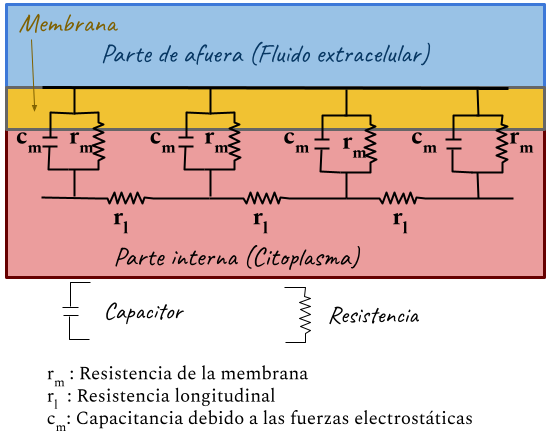
\includegraphics[scale=0.5]{../Figuras/ModeloHH.2}
 \caption{Un primer modelo de la membrana axónica modelada como circuito eléctrico. La parte amarilla es la membrana.}
 \label{fig:ModelHh}
\end{figure}


Ahora se necesitan más detalles de la representación de los canales y toman en cuenta que el comportamiento de estas resistencias viene acompañado con un voltaje de reposo, en estos voltajes particulares cada tipo de ion (de la resistencia modelada) se estabiliza y ya no va a cambiar esta resistencia (ver \ref{fig:circuito}). 


\begin{figure}[h]
 \centering
 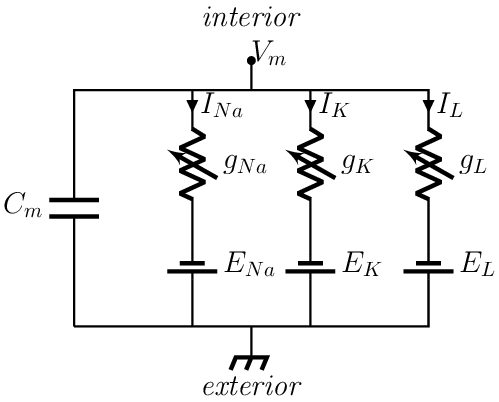
\includegraphics[scale=0.5]{../Figuras/circuito.png}
 \caption{Modelo de la membrana axónica modelada como circuito eléctrico, con los distintos canales presentes y su voltaje de reposo.}
 \label{fig:circuito}
\end{figure}

Lo que observan es que el \textbf{ion de sodio (Na+)} y su resistencia va a variar dependiendo del voltaje, a esto se le llama un \textbf{canal transitorio} porque en ciertos voltajes si puede pasar; si es muy bajo, no puede pasar y si rebasa un cierto umbral entonces se vuelve a tapar y ya no puede pasar. 
Lo que sucede con el \textbf{ion de potasio (K+)} es que, puede salir si el voltaje está más allá de un cierto valor, si no, no pasan y va variando un poquito que tanto puede pasar, a esto se le llama \textbf{canal persistente}. Por estas características de que el potasio es un intervalo dentro de la recta y el sodio es a partir de cierto valor, por tanto, se les modelan de maneras ligeramente diferentes. Más adelante se descubrió porque tenían este comportamiento, básicamente el canal de potasio es una puerta hecha de cuatro subpuertas por donde los elementos pasan o no pasan, el canal de sodio es como una compuerta que está hecha de tres subpuertas que se pueden abrir y tiene aparte un tapón extra, que hace que aunque estas tres están abiertas bloquee toda la compuerta.
Las neuronas están trabajando con muchos más iones aparte de estos dos, uno que destaca bastante es el caso del cloro (Cl-) que tiene carga negativa. Se tienen canales para intercambio aleatorio de otros iones, \textbf{L} un canal aleatorio (leaky).

Entonces con lo que ellos midieron experimentalmente, notaron cómo se estaban comportando estas resistencias dependiendo del voltaje o la diferencia de potencial que había entre ambos lados de la membrana. A partir de estas pudieron describir matemáticamente y simular los disparos que se conocen como potenciales de acción. Vamos a ver cuáles fueron estos conceptos de electricidad que se están utilizando para el modelo tenemos este concepto de potenciales eléctricos.

\begin{itemize}
\item Potenciales eléctricos \emph{E ó  V}; resultan de la separación de cargas opuestas. Se mide en \emph{mV}.
    \begin{itemize}
     \item \emph{E\textsubscript{(Na,K,L)}} voltaje en reposo para los iones de Na, K y L, o también conocido como  potencial de inversión iónico, es el potencial de membrana en el que no hay flujo neto (total) de ese ion en particular de un lado de la membrana al otro. 
     \item \emph{V\textsubscript{m}}, el potencial eléctrico de la membrana. 
     \end{itemize}

\item Corriente \emph{I}; Movimiento de cargas. Se mide en \emph{µA}.
    \begin{itemize}
     \item \emph{I\textsubscript{(Na,K,L)}} corriente entrante a los canales de Na, K o L.
     \end{itemize}

\item Resistencia \emph{R}; Medida de la oposición al movimiento de las partículas cargadas.
\item Capacitancia o capacidad eléctrica \emph{C} . Cantidad de energía eléctrica almacenada en un capacitor para una diferencia de potencial eléctrico dada.
    \begin{itemize}
     \item \emph{C\textsubscript{m}} la capacitancia de la membrana. 
     \end{itemize}

\item Conductancia \emph{g}; Inverso de la resistencia \( \dfrac{1}{R} \) , es decir, facilidad de transmisión de las partículas cargadas.
    \begin{itemize}
     \item \emph{g\textsubscript{(Na,K,L}}  la conductancia del canal de sodio, potasio, cloro y la L también refiriendose a otros canales de iones. 
     \end{itemize}

\end{itemize}

Lo que está pasando en los \textbf{potenciales eléctricos} es que hay mucho sodio en la parte externa de la membrana por ej. tres iones de sodio que son cargas positivas por dos iones de potasio que hay en la parte interna, entonces hay muchas más cargas positivas en la parte de afuera que las que hay en la parte de adentro y eso es lo que provoca la diferencia de cargas que es lo que estamos viendo como un potencial eléctrico.


La capacidad eléctrica o \textbf{capacitancia} es la que estamos utilizando para modelar la membrana conformada por lípidos, que es una capa de grasa y esa es la cantidad de energía eléctrica almacenada en un capacitor para una diferencia de potencial eléctrico dada. Éste comportamiento bastante interesante porque las cargas quedan almacenadas un momento, pero se van liberando poco a poco y se va descargando ese capacitor. 


Durante el experimento con el axón, se le dieron cargas eléctricas directamente al axón y gracias a eso lograban ir midiendo que era lo que estaba pasando con las concentraciones de cargas afuera y adentro en el caso de las neuronas reales, esto en un ambiente no alterado ocurre cuando entran en juego los neurotransmisores y provocan que haya cambios, en estas corrientes. Entonces Hodgkin y Huxley jugaron el rol que tendrían que jugar usualmente los \emph{neurotransmisores} para abrir otras compuertas. Nosotros en la manera en la que lo vamos a simular es precisamente con estas corrientes que son las que se están poniendo en el experimento y vamos a ver cómo reacciona el axón. 


\section{Potenciales de Nerst o de reposo}

Los Potenciales de Nerst o de reposo son los potenciales a los cuales el flujo neto de iones a través de los canales abiertos es cero.
Aquí vemos precisamente porque estamos utilizando la \emph{E} generalmente la vamos a utilizar para referirnos a la diferencia de potencial entre la parte de afuera de la célula y la parte de adentro, las vamos a utilizar para representar a aquellos voltajes donde cada una de las compuertas encontrarían su equilibrio. Estos voltajes son distintos para cada una de las compuertas, esto va a provocar precisamente la dinámica de la de la neurona, por ejemplo: 

\begin{itemize}
\item E \textsubscript{Na}  \emph{50mV}
\item E \textsubscript{Ca}  \emph{150mV}
\item E \textsubscript{K}   \emph{− 80mV}
\item E \textsubscript{Cl}  \emph{− 60mV}
\end{itemize}

Aquí vemos que el sodio estaría su equilibrio en un valor positivo, 
el calcio que es el que va a jugar un rol de que se activen los neurotransmisores y se transmita el disparo, observamos que el voltaje tendría que ser bastante positivo. El potasio que es el que usualmente está trabajando intercambiándose casi todo el tiempo en la neurona, veremos que el punto de equilibrio usual de la neurona anda por los $-76 mV$ y el del cloro. Cada uno de estos canales pues está tratando de jalar la dinámica hacia su potencial de equilibrio y no hay precisamente un acuerdo entre ellos y eso es precisamente lo que hace que las neuronas cobren "vida".


\section{Modelo de la membrana como bicapa de lípidos}

\hypertarget{LaEq}{La membrana} de una neurona es modelada como un elemento de un circuito con capacitancia \emph{C\textsubscript{m}} y potencial \emph{V}, las corrientes que fluye a través de la bicapa lipídica están regidos por las siguientes ecuaciones:


\begin{equation}
  I_{m} = C_{m} \dfrac{dV_{m}}{dt}
  \label{eq:corrientesEnLaMembrana}
\end{equation}

Esta sería la ecuación principal (\ref{eq:corrientesEnLaMembrana}) donde \(\dfrac{dVm}{dt}\) está representando el cambio voltaje en la membrana respecto al tiempo.

\begin{equation}
  C_{m} \dfrac{dV_{m}}{dt} =  - g_{Na} m^3 h(V - E_{Na} ) - g_{K} n 4 (V - E_{K} ) - g_{L} (V - E_{L} ) + I_ext
  \label{eq:corrientesEnLaMembrana2}
\end{equation}

Cada una de las partes del lado izquierdo de la ecuación \ref{eq:corrientesEnLaMembrana2} corresponde a las compuertas de los canales y la corriente de un estímulo externo que pueda influir a la membrana (este estímulo siempre será desde al exterior hacia el interior).

Retomando lo escrito anteriormente el canal de sodio es una compuerta compuesta de \textbf{tres} subpuertas y una subpuerta que actua como tapón y el canal de potasio es una compuerta compuesta de \textbf{cuatro} subpuertas iguales, \hypertarget{secc} {con esto podemos notar claramente que las conductancias sean representadas como}:

\begin{itemize}
 \item \(\dfrac{1}{R_{Na}} = g_{Na} * m ^3 * h \) donde \(g_{Na}\) es una constante que representa el valor de la conductancia máxima, \textbf{m} es la proporción de los canales de sodio abiertos (representa la concentración de sodio) y nos indica la activación (subpuertas abiertas) del canal, \textbf{h} es el “tapón” de la compuerta que puede impedir el paso de iones independientemente de las otras tres subpuertas, es decir la inactivación (compuerta bloqueada).
Los movimientos combinados de \textbf{m} y \textbf{h} son los que controlan la compuerta de sodio.
 \item \(\dfrac{1}{R_{K}} = g_{K} * n^4\) donde \(g_{K}\) es una constante que representa el valor de la conductancia máxima, \textbf{n} es la proporción de los canales de potasio abiertos (representa la concentración de potasio) y nos indica la activación del canal de potasio.
 \item \(g_{L}\) es una constante, de los canales por fuga, que representa la concentración de los demás iones que pasan por la membrana.
\end{itemize}

Ahora \emph{m}, \emph{n} y \emph{h}, son variables de activación que describen la probabilidad de que los canales iónicos estén abiertos, se puede describir mediante las siguientes ecuaciones diferenciales ordinarias:

\begin{equation}
  \dfrac{1}{\gamma(T)}\dfrac{dn}{dt} =  \alpha_{n^\infty} (V)(1 - n) - \beta_{n} (V) n = \dfrac{n(V)-n(t)}{\tau_{n}(V)}
  \label{eq:corrientesEnLaMembrana3}
\end{equation}

\begin{equation}
  \dfrac{1}{\gamma(T)}\dfrac{dm}{dt} =  \alpha_{m} (V)(1 - m) - \beta_{m} (V) m = \dfrac{m^\infty(V)-m(t)}{\tau_{m}(V)}
  \label{eq:corrientesEnLaMembrana4}
\end{equation}

\begin{equation}
  \dfrac{1}{\gamma(T)}\dfrac{dh}{dt} =  \alpha_{h} (V)(1 - h) - \beta_{h} (V) h = \dfrac{h^\infty(V)-h(t)}{\tau_{h}(V)}
  \label{eq:corrientesEnLaMembrana5}
\end{equation}

Donde la ecuación \ref{eq:corrientesEnLaMembrana3} representa al canal de potasio y las ecuaciones \ref{eq:corrientesEnLaMembrana4} y \ref{eq:corrientesEnLaMembrana5} representando al canal de sodio tomando en cuenta que tiene dos tipos de subpuertas.

Las expresiones de \(\alpha\) y \(\beta\) están dadas por las siguientes ecuaciones:

\begin{align*}
\alpha_{n}&=\dfrac{0.01(10-V)}{exp(\dfrac{10-V}{10})-1}           &  \beta_{n}&=0.125exp-\dfrac{V}{80}\\
\alpha_{m}&=\dfrac{0.01(25-V)}{exp(\dfrac{25-V}{10})-1}                    &  \beta_{m}&=4exp-\dfrac{V}{18}\\
\alpha_{h}&=\dfrac{0.07}{exp-(\dfrac{V}{20})}              &  \beta_{h}&=\dfrac{1}{1+exp\dfrac{30-V}{10}}
\end{align*}

Los factores \(\alpha\) y \(\beta\) se denominan como constantes de velocidad de transición. \(\alpha\) es el número de veces por segundo que se abre una puerta que está en estado cerrado, mientras que \(\beta\) es el número de veces por segundo que se cierra una puerta que está en estado abierto. Si la membrana tiene un la carga negativa, \(\alpha\) debe aumentar y la \(\beta\) debe disminuir, cuando la membrana esté despolarizada.

Hasta ahora sabemos que en la bicapa de lípidos, una pequeña carga está pasando entre sus capas de grasa. También sabemos que la carga es almacenada por un breve periodo de tiempo, dando como resultado que la bicapa se comporte como un \textbf{capacitor}. Esta membrana también está con cierta resistencia al paso de corriente. Con esto tenemos el siguiente diagrama \footnote{Otra explicación más profunda de las ecuaciones dadas partir del diagrama \ref{fig:circuitoP}la podemos encontrar en \url{https://neurowiki.case.edu/wiki/Action_Potential_IV:_Hodgkin-Huxley_Equations_and_Other_Conductances}} \ref{fig:circuitoP}

\begin{figure}[h]
 \centering
 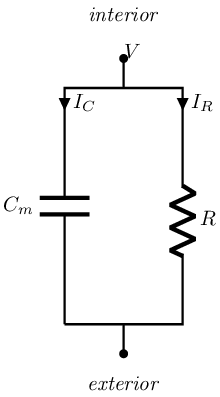
\includegraphics[scale=0.5]{../Figuras/bicapaLipidos.png}
 \caption{Modelo de la bicapa de lipidos donde, V son los cambios de voltaje en la membrana que es el potencial eléctrico, \(I_{C}\) es la corriente del capacitor, \(I_{R}\) es la corriente de la resistencia, \(C_{m}\) es la capacitancia de la membrana, R es la resistencia.}
 \label{fig:circuitoP}
\end{figure}

Tenemos dadas las siguientes ecuaciones:
\begin{equation}
    I_{C} + I_{R} - I_{ext} = 0
  \label{eq:bicapa1}
\end{equation}

\begin{equation}
    C\dfrac{dV}{dt} + \dfrac{V}{R} - I_{ext} = 0 \\
  \label{eq:bicapa2}
\end{equation}

\begin{equation*}
    C\dfrac{dV}{dt} = -\dfrac{V}{R} + I_{ext} 
\end{equation*}

Ahora por la ley de corriente de Kirchhoff \footnote{La ley de la corriente de Kirchhoff dice que la suma de todas las corrientes que fluyen hacia un nodo es igual a la suma de las corrientes que salen del nodo} tenemos que la suma de las corrientes del capacitor y la resistencia debe ser cero
por la conservación de corriente y si consideramos un factor adicional de una corriente externa aplicada o administrada a la neurona, tenemos la ecuación \ref{eq:bicapa1}.

Después tenemos la relación entre la diferencia de potenciales, que almacena energía y la carga eléctrica que guarda, donde: \emph{C} es la capacidad, medida en faradios, \emph{Q} la carga eléctrica almacenada, medida en culombios, \emph{V} la diferencia de potencial medida en voltios. Entonces \(C = Q/V\), despejando a \emph{Q} tenemos \emph{Q = CV} y derivando de ambos lados respecto al tiempo y considerando que \emph{C} es una constante al ser una propiedad de la membrana \(\dfrac{dQ}{dt} = C\dfrac{dV}{dt}\). Como la definición de corriente es el cambio de carga en el tiempo tenemos que \(I_{C} = C\dfrac{dV}{dt}\). Notemos finalmente la corriente de la resistencia \(I_{R}\), recordando la ley de Ohm \footnote{La ley de Ohm establece que la diferencia de potencial V que aplicamos entre los extremos de un conductor determinado es directamente proporcional a la intensidad de la corriente I que circula por el conductor, es decir \(V = R * I\). Notemos también que \(V = V_{m} - V_{rest}\) } la podemos rescribir como \(\dfrac{V-V_{rest}}{R}\). Sustituyendo de lo anterior en la ecuación \ref{eq:bicapa1} se obtiene la siguiente ecuación:

\begin{equation}
 C\dfrac{dV}{dt} + \dfrac{V-V_{rest}}{R} - I_{ext} = 0
 \label{eq:bicapa3}
\end{equation}

\begin{equation*}
 C\dfrac{dV}{dt} = -\dfrac{V-V_{rest}}{R} + I_{ext} 
\end{equation*}

Ahora multiplicando todo por R:
\begin{equation}
 RC\dfrac{dV}{dt} = -V + (V_{rest} + RI_{ext}) 
 \label{eq:bicapa4}
\end{equation}

Denotando RC como la constante de tiempo \(\tau\) y tomando en cuenta que en cuanto se aplica la corriente va a empezar a cambiar el voltaje poco a poco hasta establecerse en un voltaje de equilibrio (ahí se va a quedar quieta). Entonces cuando el voltaje ya no está cambiando con el tiempo quiere decir que su derivada con respecto al tiempo es cero. Observemos que \(dV/dt = 0\) significaría que V es igual a infinito y que el voltaje en el estado estacionario cuando, \(dV/dt = 0\) depende del potencial de reposo y del producto entre la resistencia con la corriente externa suministrada, entonces tenemos que:

\begin{equation}
 V_{\infty} = V_{rest} + RI_{ext}
 \label{eq:bicapa5}
\end{equation}

Sustituyendo con \ref{eq:bicapa5} y la constante, en \ref{eq:bicapa4} tenemos que:
\begin{equation}
 \tau\dfrac{dV}{dt} = -V + V_{\infty}
 \label{eq:bicapa6}
\end{equation}

\subsection{Las conductancias iónicas}
Nuestro objetivo aquí es encontrar ecuaciones que describan las conductancias con precisión razonable y lo suficientemente simples para el cálculo teórico de \emph{el potencial de acción} y \emph{el período refractario}. 

Si tomamos las ecuaciones diferenciales anteriores notamos que las soluciones tienen este tipo de forma \ref{fig:graficaX}:

\begin{figure}[h]
 \centering
 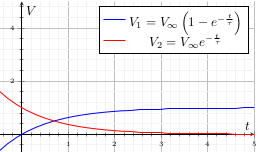
\includegraphics[scale=0.8]{../Figuras/solPulso1.png}
 \caption{Soluciones para el pulso.}
 \label{fig:graficaX}
\end{figure}


Donde si estamos aplicando una corriente externa lo que sucede es lo que estamos viendo en azul, un exponencial que va creciendo y que tiende hacia un cierto valor límite que sería de infinito. Si dejamos de aplicar la corriente externa entonces ahora tendremos un exponencial, pero que tiende hacia el cero y se va a estabilizar en cero, lo que vemos en rojo. 

\begin{figure}[h]
 \centering
 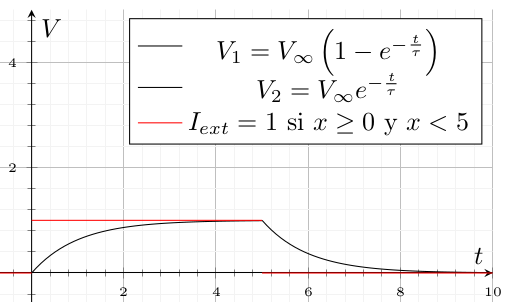
\includegraphics[scale=0.5]{../Figuras/solPulso2.png}
 \caption{Soluciones para el pulso escalón.}
 \label{fig:graficaX1}
\end{figure}

Simulando lo que hicieron Hodgkin y Huxley que fue al axón de repente darle un toque, siendo en el origen de la gráfica (que visualizamos en la figura \ref{fig:graficaX1}) la parte en la que le están dando el toque al axón, momentos antes estaba quieta la neurona de repente le aplican una cierta cantidad de electricidad y va a empezar a cambiar el comportamiento de los canales la porosidad de la membrana, vamos a ver que empieza a incrementarse la diferencia de potencial hasta que llegan a un nuevo equilibrio (alrededor de t = 3) y si siguieran dándole el toque en esa cantidad se quedaría ahí la neurona, ya no veríamos más cambios lo que va a suceder entonces es que, retiramos las pinzas (se le deja de dar el toque) y los canales otra vez van a empezar a regresar a la normalidad y vamos a ver un descenso en adelante.

Entonces hasta aquí ya tenemos la idea de cómo va a reaccionar la neurona ante cierto estímulo; sin embargo, esto que acabamos de ver en las gráficas sería como si tuviéramos un solo tipo de canal, ahora qué pasa si consideramos que tenemos diferentes tipos de canales pasando iones, en condiciones distintas. 
Aquí es donde va a importarnos el hecho de que existen diferentes tipos de canales con voltajes de equilibrio diferente. 
Retomando a los potenciales de Nerst \(E_{Na},E_{K},E_{L}\) notemos que están dados por:


\begin{equation}
    E = \dfrac{k_{B}T}{zq}\ln\dfrac{[adentro]}{[afuera]}
 \label{eq:diferenciaP}
\end{equation}

Estos potenciales están relacionados con las características termodinámicas, en la ecuación anterior \ref{eq:diferenciaP} \(k_{B}\) la constante de Boltzman, \(q\) es la carga del ion, y \(z\) es el número de iones. El logaritmo natural representando el promedio de cuántos elementos tenemos en la parte de adentro con respecto a cuántos elementos tenemos en la parte de afuera.

Considerando los diferentes puntos de equilibrio en los cuales se puede encontrar la diferencia de potencial en la membrana, vamos a distinguir entre tres estados de esta (también se puede ver en \ref{fig:graficaP}):

\begin{enumerate}
 \item \textbf{Polarizada} en su estado de reposo con \(V < 0 ( V \approx -70 mV )\).
 \begin{itemize}
  \item Su estado de reposo,cuando la neurona no está haciendo nada simplemente están corriendo los sodios y entran los potasios.
 \end{itemize}
 \item \textbf{Despolarizada} cuando \(V \geq 0\).
 \begin{itemize}
  \item Cuando en sus dendritas y en el cuerpo de la neurona se acumula una carga muy grande (un voltaje electrico, disparo), se abre la compuerta de sodio y van a empezar a entrar el sodio, esta diferencia de potencial que existía entre lo fuera y lo adentro se va a reducir de hecho se puede llegar a reducir bastante dependiendo de la carga que se le aplique.
  \item Iones positivos entran a la membrana.
  \item Valores positivos en la diferencia de potencial.    
 \end{itemize}
 \item \textbf{Hiperpolarizada} cuando la diferencia de potencial incrementa su magnitud \(V << 0\).
 \begin{itemize}
 \item En cuanto se despolarice van a empiezar interacciones entre los diferentes tipos de canales que lo que van a intentar hacer es regresar a la neurona en su estado normal.
 \item Los canales de potasio abren sus compuertas, provocando que salga el potasio que está dentro del axón (en el citoplasma). 
 \item Iones positivos salen de la membrana.
 \item Si antes estaba quieta a los - 70mV, ahora va a quedar todavía más abajo alrededor de - 90mV. Esto va a permitir un fenómeno que se le conoce como \emph{el periodo de refracción} y ese periodo sirve para que simplemente se lance un disparo y que el comportamiento eléctrico no se rebote otra vez en dirección contraria en la neurona, va a quedar muy quieta la neurona durante un rato y después regresará otra vez a su estado de equilibrio. 
 \end{itemize}

\end{enumerate}
 
\section{Modelo de las compuertas iónicas controladas por voltaje}

Retomando el modelo del circuito eléctrico modelando la membrana, junto con los canales y los iones, volvamos a verlo ahora en la \ref{fig:circuito1}

\begin{figure}[H]
 \centering
 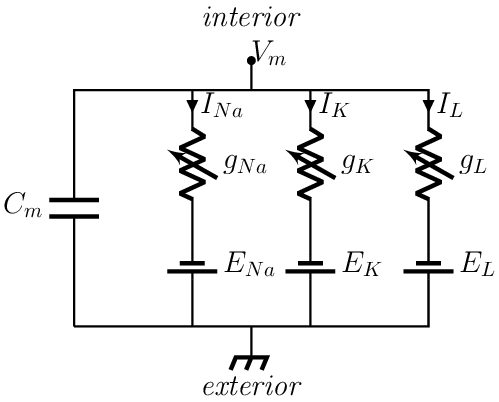
\includegraphics[scale=0.5]{../Figuras/circuito.png}
 \caption{Modelo de la membrana axónica modelada como circuito eléctrico, con los distintos canales presentes y su voltaje de reposo.}
 \label{fig:circuito1}
\end{figure}

Recordemos brevemente las definiciones de los dos tipos de canales protagonistas en el modelo:

\begin{definition}
 \emph{Canal persistente} Tiene un solo tipo de compuerta y dos estados posibles:
 \begin{enumerate}
  \item \textbf{Activado}
  \item \textbf{Desactivado}
 \end{enumerate}

\end{definition}

\begin{definition}
 \emph{Canal transitorio} Tiene compuertas de activación e inactivación, y tres estados:
 \begin{enumerate}
  \item \textbf{Activado} Ambas compuertas abiertas.
  \item \textbf{Desactivado} Compuerta de activación cerrada, inactivación abierta.
  \item \textbf{Inactivada} Compuerta de inactivación cerrada.
 \end{enumerate}

\end{definition}


Y retomando \hyperlink{LaEq}{la primera ecuación diferencial} donde tenemos, por un lado, la corriente que está pasando a través del capacitor, por otro lado, vamos a tener las corrientes que están circulando a través de los diferentes canales, 

\begin{equation}
  C_{m} \dfrac{dV_{m}}{dt} = - g_{Na} m^3 h(V_{m} - E_{Na}) - g_{K} n 4 (V_{m} - E_{K}) - g_{L} (V_{m} - E_{L}) + I_{ext}
  \tag{\ref{eq:corrientesEnLaMembrana2}}
\end{equation}

Las capacitancias y variables del lado izquierdo están explicadas en la sección \hyperlink{secc}{\emph{Modelo de la membrana como bicapa de lípidos}}, aqui vamos a retomar las ecuaciones \ref{eq:corrientesEnLaMembrana3},\ref{eq:corrientesEnLaMembrana4},\ref{eq:corrientesEnLaMembrana5} de esa misma sección, (recordemos que estás ecuaciones describen la probabilidad de que los canales iónicos estén abiertos) que son las siguientes:

\begin{equation}
  \dfrac{1}{\gamma(T)}\dfrac{dn}{dt} =  \alpha_{n^\infty} (V)(1 - n) - \beta_{n} (V) n = \dfrac{n(V)-n(t)}{\tau_{n}(V)}
  %\label{eq:probabilidades1}
  \tag{\ref{corrientesEnLaMembrana3}}
\end{equation}

\begin{equation}
  \dfrac{1}{\gamma(T)}\dfrac{dm}{dt} =  \alpha_{m} (V)(1 - m) - \beta_{m} (V) m = \dfrac{m^\infty(V)-m(t)}{\tau_{m}(V)}
  %\label{eq:probabilidades2}
  \tag{\ref{corrientesEnLaMembrana4}}
\end{equation}

\begin{equation}
  \dfrac{1}{\gamma(T)}\dfrac{dh}{dt} =  \alpha_{h} (V)(1 - h) - \beta_{h} (V) h = \dfrac{h^\infty(V)-h(t)}{\tau_{h}(V)}
  \tag{\ref{corrientesEnLaMembran53}}
\end{equation}

Ahora notemos los elementos en estas ecuaciones anteriores con \(ion\) pudiendo denotar las compuertas del potasio \(n\) o del sodio, ya sea \(m\) o \(h\):
\begin{itemize}
 \item \(\dfrac{1}{\gamma(T)}\) Este es el coeficiente de escala temporal, dependiente de la temperatura los por eso está apareciendo aquí una \(t\). Para las simulaciones que nosotros vamos a hacer vamos a pensar que estamos en una temperatura fija. 
 \item \(\alpha_{ion}(V)\) probabilidad de que una compuerta transite de cerrada a abierta.
 \item \(\beta_{ion}(V)\) probabilidad de que una compuerta transite de abierta a cerrada.
 \item \(ion^\infty(V)\) probabilidad de compuerta abierta en el equilibrio cuando \(t \rightarrow \infty\).
 \item \((ion)\) Probabilidad de que cada compuerta (n, m, h) esté abierta.
 \item \((1-ion)\) Probabilidad de que cada compuerta (n, m, h) esté cerrada.
 
 \item \(\tau_{ion}(V)\) Tiempo que toma llegar al equilibrio.
\end{itemize}


Lo que vamos a ver es que forma de escribir la ecuación depende precisamente del número de compuertas que tenían para poder abrirse y cerrarse. Reescribir la ecuación de esta manera lo que nos permite es medirlo en términos de estas probabilidades de que se abran y cierren las compuertas que serían 

Esta probabilidad se empieza a alterar conforme cambiamos el voltaje, pero no va a llegar a su valor de equilibrio sino hasta después de pasado un cierto periodo.


\section{Dinámica del voltaje durante un disparo} 

Ahora qué pasa cuando tomamos en cuenta que todas las compuertas están reaccionando al mismo tiempo.
Notemos primeramente como está reaccionando la membrana ante un impulso electrico o voltaje, en la siguiente imagen \ref{fig:voltaje1}.

\begin{figure}[h]
 \centering
 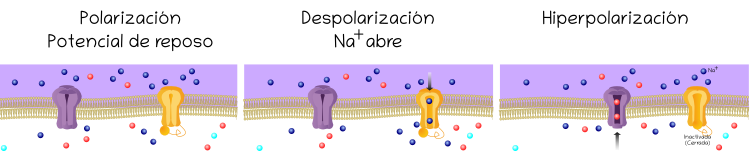
\includegraphics[scale=0.5]{../Figuras/polarizacion1.png}
 \caption{En la primera parte los canales están en un estado de reposo y la membrana está polarizada. En la segunda parte los canales han sido afectados por un impulso recibido desde el cono axónico, las compuertas de sodio se abren permitiendo el paso de iones de sodio al interior de la membrana y dejando a la membrana despolarizada. Momentos después la membrana llega a un estado de hiperpolarización donde intentará regresar al estado de equilibrio que tenía previamente, para esto la subpuerta de inactivación de sodio cerrará hasta no permitir el paso de sodio y el canal de potasio abrirá sus compuertas para dar salida a los potasios (iones positivos) que fluyan hacia el exterior de la membrana, así dejando el voltaje de la membrana incluso más negativo de lo que tenía durante su estado polarizado. }
 \label{fig:voltaje1}
\end{figure}

Ahora lo que vemos en la imagen \ref{fig:voltaje1} se grafica de manera un poco más apegada a lo que pasa en los experimentos de la siguiente forma en la imagen \ref{fig:voltaje2}.

\begin{figure}[h]
 \centering
 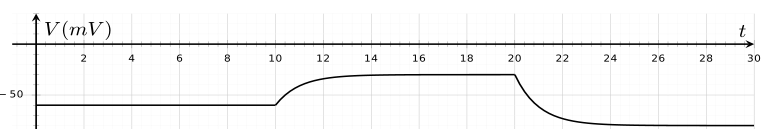
\includegraphics[scale=0.5]{../Figuras/polarizacion2.png}
 \caption{Gráfica del cambio de voltaje en la membrana dado un impulso atrevés del tiempo. Cuando se rebasa el voltaje umbral, los canales de Na + y K + interactúan para producir una rápida despolarización de la membrana provocando una elevación del voltaje, para luego hiperpolarizarla. Durante el momento de despolarización la membrana puede llegar a valores positivos en este caso en particular el estímulo no es tan grande y se queda en valores negativos.}
 \label{fig:voltaje2}
\end{figure}


Ahora lo anterior está en términos de lo deseado, veamos entonces que paso en las mediciones de Hodgkin y Huxley con el axón en las siguientes gráficas \ref{fig:voltajeAB}, donde nos está mostrando como las subpuertas n y los factores \(\tau\), \(\alpha\) y \(\beta\) del canal de potasio se comportaron antes, durante y después del estímulo del voltaje. Recodemos que \emph{n} nos indica la probabilidad que las compuertas de potasio estén abiertas, este es un factor adimensional. \(\tau\) es el tiempo que tarda en llegar a un estado de equilibrio. \(\alpha\) y \(\beta\) las probabilidades que las compuertas del canal de potasio pasen de cerrados a abiertos y viceversa. 


Entonces notamos que en el mismo periodo de tiempo, la membrana está en reposo y conforme va recibiendo el voltaje incrementa la probabilidad que las compuestas de potasio estén abiertas, es decir \(n\) va incrementando conforme al estímulo, mientras que el estado de reposo es claramente alterado provocando que el valor \(\tau\) disminuya considerablemente. La probabilidad que las compuertas de potasio pasen de un estado cerrado a uno abierto durante el proceso (\(\alpha\)) aumenta prácticamente de forma exponencial, mientras que la probabilidad de que pasen de abierto a cerrado disminuye poco a poco. Con esto cumpliendo lo esperado en la dinámica del voltaje, al notar como está reaccionando el canal de potasio durante la polarización y despolarización (pulso). 



\begin{figure}[h]
 \centering
 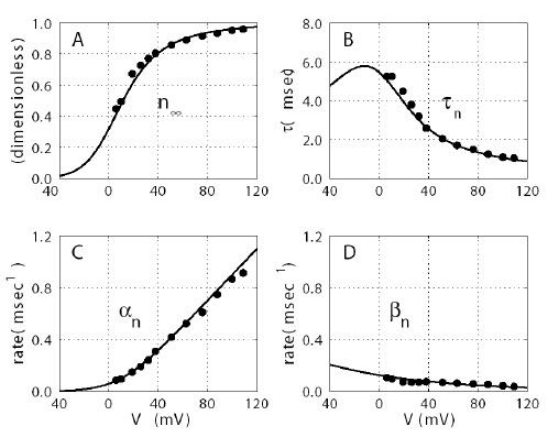
\includegraphics[scale=0.5]{../Figuras/medidasExperimentales.png}
 \caption{Medición experimental de los parámetros y ajuste manual de curvas. Imagen de Nelson 2004}
 \label{fig:voltajeAB}
\end{figure}

Con estas medidas experimentales ellos dan con curvas paramétricas ajustadas a los factores \(\alpha\) y \(\beta\) expresadas de la siguiente forma:

\begin{align*}
\alpha_{n}&=\dfrac{0.01(10-V)}{e^{\left(\dfrac{10-V}{10}\right)}-1}           &  \beta_{n}&=0.125e^{-\dfrac{V}{80}}\\
\alpha_{m}&=\dfrac{0.01(25-V)}{e^{\left(\dfrac{25-V}{10}\right)}-1}                    &  \beta_{m}&=4e^{-\dfrac{V}{18}}\\
\alpha_{h}&=0.07 e^{-\left(\dfrac{V}{20}\right)}              &  \beta_{h}&=\dfrac{1}{e^{\left(\dfrac{30-V}{10}\right)}+1}
\label{eq:curvas}
\end{align*}


Ahora veamos las gráficas de la dinámica del disparo pero ya con los las compuertas del potasio y sodio interactuando al mismo tiempo, en las figuras \ref{fig:voltajeActInac} y \ref{fig:voltajeActInac1}


\begin{figure}[h]
 \centering
 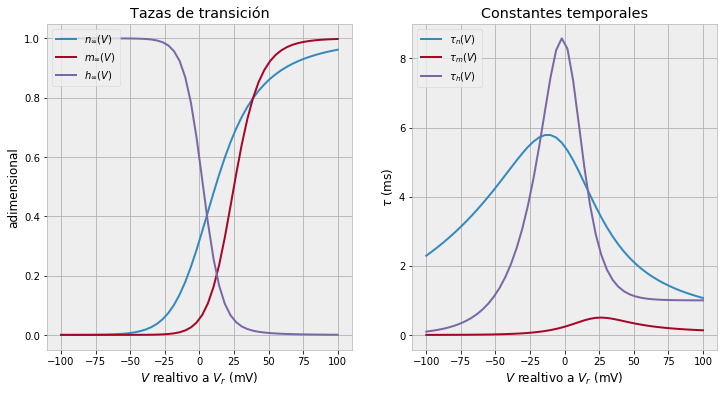
\includegraphics[scale=0.6]{../Figuras/actinac.png}
 \caption{Activación e inactivación de los canales. Del lado izquierdo vemos que alrededor de los -50 mV aumenta la probabilidad que las compuertas de potasio abran y los potasios salgan, el sodio tarda un poco más en reaccionar para dejar entrar a los sodios, y la probabilidad que quede no bloqueado disminuye, hasta bloquear por completo a los iones de sodio alrededor de los 50 mV. Del lado derecho vemos como \(\tau\), va interactuando conforme al voltaje, el Na+ reacciona rápidamente ante él impuso pues regresa rápidamente a su estado de equilibrio, esto indica porque aún que el sodio abre sus compuertas, la compuerta de bloqueo se cierra rápidamente, dejando inactivado el canal, luego el K+ reacciona más lentamente para regresar a su estado de equilibrio dejando más tiempo activado el canal y salgan los potasios.}
 \label{fig:voltajeActInac}
\end{figure}


\begin{figure}[H]
 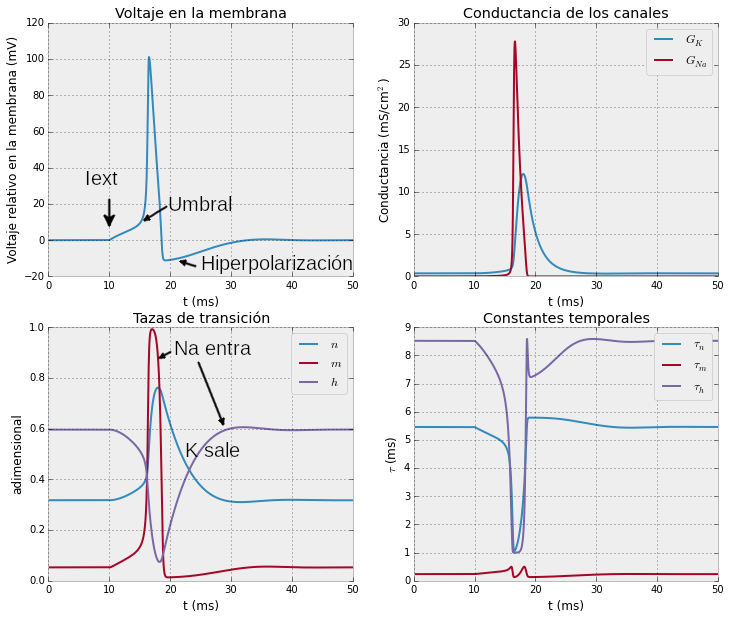
\includegraphics[scale=0.6]{../Figuras/disparo.png}
 \caption{Medidas experimentales del estímulo y la reacción de todos los componentes de la membrana. El origen en estás gráficas realmente esta representando el punto de equilibrio que es alrededor de los -70mV. Del lado superior izquierdo mostrando como cambia el voltaje de la membrana respecto al tiempo, del lado superior derecho el comportamiento de la conductancia de los canales mostrando que aunque la conductancia del sodio reacciona más, es más breve, mientras que el potasio reacciona en menor medida pero durante más tiempo. En la parte inferior derecha la taza de transición de las compuertas n,m y h, mostrando que en cuando llega el impulso el primero en reaccionar es el sodio permitiendo que entre muy brevemente el sodio e inactivandose casi inmediatemente después, mientras que en ese momento los potasios se están liberando hacia la parte exterior de la meurona. Finalmente del lado inferior izquierdo mostrando como se comporta las constantes temporales, mostrando que las compuertas de activación de sodio no son tan afectadas comparado a la compuerta de bloqueo, notando algunos cambio bruscos en esta, mientras que el potasio si se nota más afectado y durante más tiempo pero recuperandose sin cambios bruscos. }
 \label{fig:voltajeActInac1}
\end{figure}




\section{Simulación usando el método de Euler}

En esta sección se listará como estamos resolviendo las ecuaciones diferenciales, para tener una simulación numérica y se trata del algoritmo de integración \footnote{Hodgkin-Huxley Simulation Using Euler's Method lo puedes encontrar en la siguiente liga \url{https://webpages.uidaho.edu/rwells/techdocs/Biological\%20Signal\%20Processing/Chapter\%2003\%20The\%20Hodgkin-Huxley\%20Model.pdf}}. Las gráficas de la sección anterior se obtuvieron con el método de Euler que se describe más adelante.

\begin{algorithm}
  \caption{Algoritmo de integración de Euler [Wells pp51].}\label{AIE}
  \begin{algorithmic}[1]
    \Function{INTEGRADISPARO}{$T,\Delta T,V_{0},I_{ext}(t)$}
    \State Inicializar arreglos de logitud T: $T[],V[],n[],m[],h[],G_{Na}[],G_{K}[],\tau_{n}[],\tau_{m}[],\tau_{h}[] \gets arreglo[numeroDePasos] $
    \State  $V[0] \gets V_{0}$
    \For {$ t = 0  a  t = T cada \Delta t $}
        \State Calcular $\alpha_{n}, \beta_{n}, \alpha_{m}, \beta_{m},\alpha_{h}, \beta_{h} $ utilizando $V(t)$.
        \State Calcular las tres $\tau_{x} $ y $x^\infty $ apartir de las anteriores.
        \State Calcular las probabilidades de las compuertas $n, m, h, $ utilizando las ecuaciones en diferencias en su forma matricial $\Pi(t + \Delta t) = A_{\pi}\Pi(t) + B_{\pi}$.
        \State Calcular $G_{Na} = g_{Na}m^3h $ y $G_{K} = g_{K}n^4 $.
        \State Almacenar los resultados de este paso en los arreglos $T[], V[], n[], m[], h[], G_{Na}[], G_{K}[], \tau_{n}[], \tau_{m}[], \tau_{h}[] $
        \State $I_{ext} \gets I_{ext}(t) $
        \State Calcular $V_{m} (t + \Delta t) $
    \EndFor
    \State Devolver los arreglos $T[],V[],n[],m[],h[],G_{Na}[],G_{K}[],\tau_{n}[],\tau_{m}[],\tau_{h}[] $ con los resultados para los tiempos $[0,T] $
    \EndFunction
  \end{algorithmic}
\end{algorithm}


Comenzamos con un valor inicial y a partir de ahí empleamos las ecuaciones, para calcular las tangentes, aproximamos a la curva con su tangente.

Para la función \textproc{INTEGRADISPARO} necesitamos cuatro valores de entrada que van a provocar diferentes comportamientos:

\begin{enumerate}
 \item $T$ nos indica durante cuánto tiempo queremos correr la simulación.
 \item $\Delta T $ nos indica que tan finos queremos que sean los pasos recordemos que vamos a aproximar la función con segmentos de recta siguiendo la tangente. Si hacemos pasos demasiado pequeños nos vamos a tardar demasiado en hacer el cómputo.
 \item $V_{0} $ es el voltaje inicial en donde empieza nuestra simulación donde estaba en nuestra neurona cuando empezamos a trabajar.
 \item $I_{ext}(t) $ es la corriente externa, de qué magnitud fue el toque que le estamos dando en este momento al axón 

\end{enumerate}

A partir de los elementos iniciales proporcionados ya podemos calcular lo demás. Vamos a querer guardar lo que está ocurriendo para todos los tiempos desde cero hasta t en cada delta, y lo vamos a hacer en forma de arreglos donde en la posición [0], está la primera medición en t=0 y la posición t está la medición en el tiempo t. Vamos a tener toda una serie de puntos donde estamos guardando estos pasos para inicializarlo. 

Sabemos que necesitamos es un primer valor a partir del cual vamos a calcular la tangente y vamos a ir aproximando lo demás, entonces para eso queríamos \emph{el voltaje inicial}, como nosotros sabemos donde estaba en reposo nuestra célula originalmente, vamos a poder guardar ese voltaje como el primer valor para nuestra simulación. Ahora todos los demás elementos como $\alpha$s y $\beta$s y etc. se pueden calcular si ya conocíamos ese voltaje inicial, entonces a partir de este momento podemos repetir el mismo ciclo tantas veces como sea necesario para cubrir, el intervalo. 
Desde el tiempo inicial hasta el tiempo t, brincando de delta T en delta T. 
Entonces dado un voltaje vamos a calcular las diferentes \(\alpha\)s que son las que se medían experimentalmente originalmente utilizando las ecuaciones  de las curvas paramétricas ajustadas \ref{eq:curvas} (paso 5).

Ya calculadas las alfas y betas ahora si se puede calcular las $\tau$ , $n^{\infty}$, $m^{\infty}$, $h^{\infty}$ (paso 6).
Teniendo estas entonces podemos calcular las probabilidades para las compuertas n, m, h usando las ecuaciones en diferencias en forma matricial, estas matrices se pueden expresar como \ref{fig:matriX}.

\begin{figure}[H]
 \centering
 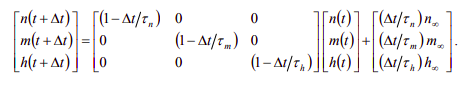
\includegraphics[scale=0.7]{../Figuras/matrix.png}
 \caption{Forma matricial para el cálculo de las probabilidades de las compuertas n, m, h.}
 \label{fig:matriX}
\end{figure}

Ahora esta parte fue importante sobre todo por el asunto de las pérdidas numéricas, recordemos que la computadora tiene una representación en punto flotante, lo cual quiere decir que un número real no se puede representar en la computadora, esto es importante por el problema del truncamiento, cada vez que se truncan dígitos al momento de calcular estamos perdiendo precisión, por esto es importante la forma en la que se procede a hacer los cálculos porque puede que se llegue a resultados un tanto distintos a los deseados aunque los cálculos sean correctos. 

Ya teniendo estos datos podemos fácilmente calcular las conductancias, simplemente sustituyendo los valores (paso 8).

Es bueno una vez que ya terminamos de calcular estos términos que se van a necesitar en la ecuación principal  \ref{eq:corrientesEnLaMembrana2} que es la del voltaje de la membrana,  ir almacenando en los \emph{resultados temporales} dentro de nuestros arreglos en la casilla que les corresponda, para ese momento (paso 8). En el paso 9, es donde ya vamos a utilizar \emph{la corriente externa} para meterla en la ecuación diferencial para el voltaje. Una vez que tengamos esto tenemos que repetirlo para cada paso, se está calculando el tiempo t,  entonces conforme avance el tiempo, va a dar el siguiente valor del voltaje, ya teniendo el siguiente valor del voltaje se va a poder usar para el siguiente paso ("como valor inicial nuevo") y así nos vamos a seguir todo el tiempo. 
Terminando el tiempo asignado a la simulación, tenemos ya los arreglos llenos de los datos que nos van a poder permitir graficar, qué fue lo que sucedió en cada tiempo, con cada canal y es precisamente  así que se puede graficar las mediciones presentadas en la sección anterior.


\section{Información condificada en las dendritas}

En esta última sección de este capítulo, se va a tratar el cómputo en las neuronas, que vamos a simplificar para poder modelar las neuronas artificiales. Ya vimos detalladamente que pasa a lo largo del axón de la neurona, se ha mencionado que son quienes conforman la región que recibe la información (disparos / pulsos). Estos mandados desde los botones de las terminales de las neuronas presinápticas y son las dendritas las encargadas de enviar estas señales hasta el soma de la neurona y hacer que estas señales químicas se transformen o no en impulsos eléctricos. Ahora la siguiente cuestión es ¿Podemos hacer que se dispare más de una vez (con el mismo estímulo)?.

Los disparos que produzca una neurona depende fuertemente de la interacción con sus neuronas vecinas. Recordemos que durante el período refractario lo que sucede, es que cuando se acumula información en las periferias del cuerpo de la neurona a través de las dendritas y de su cuerpo es porque; está recibiendo información de neuronas vecinas y eso va a hacer que dispare.

Algunas neuronas tienen el periodo de refractario muy pequeño y disparan frecuentemente, por las conexiones que tienen con sus vecinas, son neuronas que mandan frecuentemente información y a veces pueden lanzar una serie de pulsos muy seguidos, en
otras ocasiones puede haber interrupciones entre estas series de pulsos (ver imagen \ref{fig:neuronStaining}, en caso de los seres humanos podemos referirnos a las neuronas motoras que están en constante recepción y transmisión de información).

\begin{figure}[h]
 \centering
 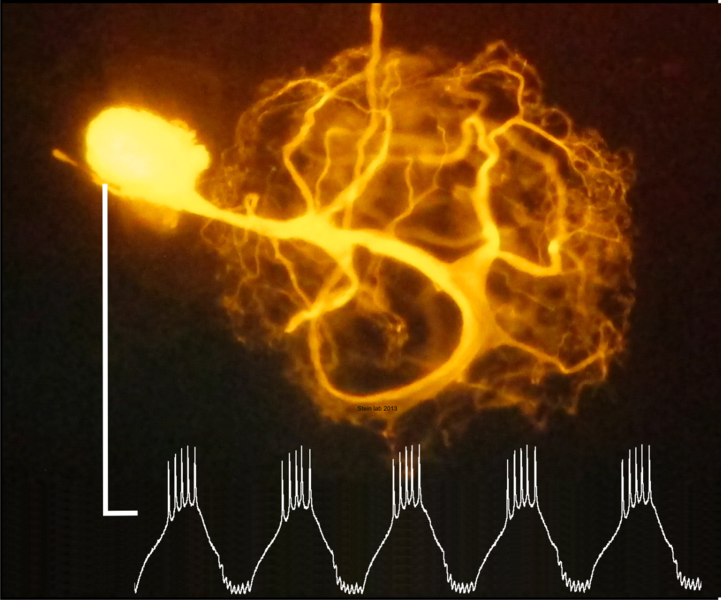
\includegraphics[scale=0.7]{../Figuras/neuron_staining_and_recording.png}
 \caption{Disparos de una neurona, Wstein, 14 September 2013, Wikimedia Commons. Esta foto muestra la neurona de cangrejo que se tiñó mediante la inyección intracelular de un colorante fluorescente. El recuadro muestra una grabación de las oscilaciones rítmicas del potencial de membrana. Las grabaciones fueron realizadas por Christopher Goldsmith en el laboratorio de Wolfgang Stein en la Universidad Estatal de Illinois, \url{https://upload.wikimedia.org/wikipedia/commons/c/ca/PD_neuron_staining_and_recording.png} , CC BY-SA 3.0.}
 \label{fig:neuronStaining}
\end{figure}

Por otro lado, hay otras neuronas que son muchísimo más pasivas y disparan muy rara vez (neuronas que están a niveles más altos, como reconocimiento de olores, colores, imágenes). Y también nos encontramos con casos donde aparentemente una neurona no reacciona ante ningún estímulo, hasta que pasa un estímulo muy especifico \footnote{Neuronas individuales que forman conceptos abstractos, responden por ejemplo, al nombre de un ser humano. Es así como se descubrió la neurona ‘Jennifer Aniston’, que disparaba cada vez que el retrato de la actriz se mostraba a los sujetos. Estas neuronas, que responden ante la presentación de algunas imágenes recibieron la denominación de“células abuelas”.} y está dispara (neuronas conceptuales o aisladas). La comunidad científica aún no se atreve a afirmar si este tipo de neurona solo dispara ante ese estímulo específico, o simplemente se trata de un evento que cumple con todas las condiciones para que esta neurona reaccione y mande un pulso. Cabe mencionar que estas neuronas se encuentran en las capas más altas de abstracción de procesamiento del cerebro \footnote{En la siguiente liga se puede encontrar información más detallada acerca de la investigación con estas neuronas: \url{https://www.nature.com/articles/s41598-020-64466-7}}. Este tipo de diferencias entre neuronas te será más fácil recordar si regresas a la última sección del primer capítulo donde se encuentra un diagrama de los procesos de información en los que puede invertir una neurona, este diagrama es \ref{fig:zonasFun}.

En este momento notamos la gran importancia de la codificación de la información en las redes neuronales de un cerebro. Donde la frecuencia de potenciales de acción nos muestran, ciertos patrones que nos indican el nivel de abstracción al que está respondiendo la neurona y el tipo de información que ayuda codificar o decodificar. 

Teniendo ahora noción del papel que juegan los patrones de la frecuencia de disparos, se han hecho numerosas investigaciones acerca de estos. En un intento de entender mejor como es que un cerebro recibe la información desde el exterior, procesa y finalmente provoca ciertas reacciones ante el estímulo. En la siguiente imagen \ref{fig:simpleModel} que es el resultado de un artículo donde se utilizaron diferentes métodos para simular disparos de neuronas y notamos la clasificación de estos patrones que se dan ante ciertos estímulos. Cada uno de estos patrones, están codificando cosas distintas, donde una misma neurona podría alternar entre diferentes patrones dependiendo de cuál es el estímulo que está recibiendo.
Si bien ha habido algunas propuestas donde se tratan de hacer neuronas artificiales que tomen en cuenta la frecuencia de disparos aún hay un amplio campo de investigación en este tema.

\begin{figure}[h]
 \centering
 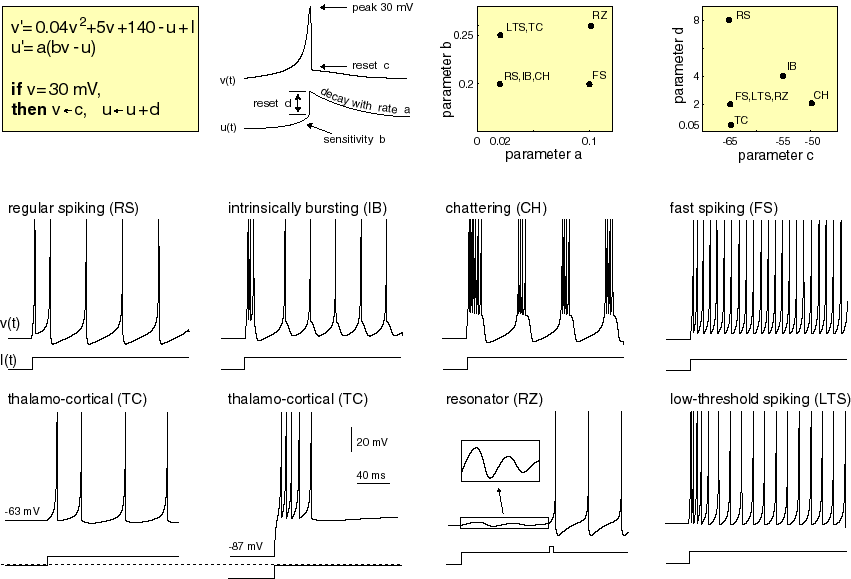
\includegraphics[scale=0.5]{../Figuras/Simple_Model_of_Spiking_Neurons.png}
 \caption{Diferentes patrones de disparo (simulados), Eugene M. Izhikevich, 2003, The Neurosciences Institute, \url{http://www.izhikevich.org/publications/spikes.html}}
 \label{fig:simpleModel}
\end{figure}

Por último mostremos la situación del sistema auditivo con la siguiente imagen \ref{fig:sonidoDisp}:

\begin{figure}[H]
 \centering
 \includegraphics[scale=0.4]{../Figuras/Localización_del_sonido_por_disparidad.png}
 \caption{Localización del sonido por disparidad, Ian Stevenson, 7 enero 2008, El sistema auditivo registra y analiza pequeñas diferencias en el tiempo de llegada de los sonidos a los dos oídos para estimar la dirección desde la cual el sonido es emitido, \url{http://www.scholarpedia.org/w/images/4/4d/JeffressFig1.png}}
 \label{fig:sonidoDisp}
\end{figure}

La imagen muestra cómo computan las neuronas, este ejemplo se trata del sistema de audio humano. Cuando nosotros oímos podemos tratar de inferir aproximadamente desde donde está siendo emitido el sonido y eso se logra gracias a que tenemos neuronas conectadas al área auditiva (tanto con el oído derecho como con el oído izquierdo). La señal auditiva va a tardar más en llegar a un oído que al otro, dependiendo de su posición en el espacio, por lo que el cerebro siempre tratar de calcular ese desfase.  
En el esquema se representa como dentro del espacio de una persona se encuentra una fuente de sonido. Dependiendo de la dirección que provenga (izquierda o derecha), las neuronas receptoras de cada oído harán un cálculo rápido de la distancia a la que se percibió la señal, estás llegaran al cerebro y en algún punto enlazaran con neuronas donde estás cuentan las diferencias de distancias percibidas hasta llegar a dar con el resultado, dándonos a saber cuáles receptores (izquierda o derecha) están más cerca de la señal, y así ubiquemos desde donde proviene el sonido.




\chapter{Aprendizaje de máquina}
\section{Introducción}

En este capitulo se desarrolla el procesos que pasa una maquina para que "aprenda", para esto notemos el concepto de aprender. En lo seres humanos se denota como el hecho de adquirir el conocimento de algo mediante el estudio o la experiencia a partir de ejemplos específicos en nuestro medio, entonces aquellos problemas que inicialmente no pueden resolverse, puedan ser resueltos después de obtener más información acerca del problema. Desde pequeños empezamos por aprender por palabras (conceptos) que asociamos con algo especifico, para después relacionar que varios objetos pertenecen a un tipo de conjunto y otros no. Como que un muñeco, una pelota y unos bloques de construcción de plastico, pertecen a un conjunto denotado como "juguetes", y que plato, taza, y tazón no pertecen a este conjunto sino al conjunto "vajilla". Entonces para organizar los conceptos que vamos aprediendo hacemos uso de una función booleana, donde la entrada es el concepto, la pregunta es, ¿Este objeto pertence a un cierto conjunto de objetos con características similares? y la salida es falso o verdadero. A este proceso, se le conoce como \emph{aprendizaje de conceptos} y en este curso lo simplificamos como \emph{función boleana de aproximación mediante ejemplos}.

Ahora lo que denotamos como el hecho que una maquina aprenda, lo vemos como cualquier programa que mejore su desempeño en alguna tarea mediante la experiencia. Con más formalidad se denota como:

\begin{definition}
 \textbf{Apredizaje maquina:} Se dice que un programa de computadora aprende, si su desempeño en T, medido por P , mejora con la experiencia E. Tal que: 

 \begin{itemize}
  \item \emph{T} es un tipo de tarea, como:
   \begin{itemize}
    \item Jugar un juego de mesa.
    \item Clasificar varios tipo de hojas.
    \item Reconocer una voz en particular.
   \end{itemize}
  \item \emph{P} es una medida de desempeño, como:
    \begin{itemize}
     \item Porcentaje de juegos ganados en las partidas.
     \item Porcentaje de hojas correctamente clasificadas.
     \item Porcentaje de reconocimiento de timbre de la voz.
    \end{itemize}
  \item \emph{E} la experiencia con ejemplos (entrenamiento), como:
    \begin{itemize}
        \item Jugar juegos de práctica.
        \item Una secuencia de imagenes etiquetadas.
        \item Una secuencia de audios etiquetados.
    \end{itemize}
    

 \end{itemize}

 , \footnote{Machine Learning, Mitchell 1997, pag. 14.}.
\end{definition}

A partir de ahora nos dedicaremos a definir correctamente tareas que nos interese que un programa aprenda, para entender la forma más abstracta del problema y así proponer los algoritmos que nos ayuden a resolverlo.

Consideremos también que los sistemas de redes neuronales artificiales son un tipo de algoritmo para la representación del proceso de aprendizaje. Un problema de aprendizaje bien definido requiere una tarea bien especificada, medidas de desempeño y datos para obtener experiencia. 

El aprendizaje maquina se apoya de disciplinas, como la inteligencia artificial, probabilidad, estadística, complejidad computacional, psicología, neurobiología y filosofía.

Para proponer un algoritmos de aprendizaje automático necesitamos, elegir el tipo de experiencia de entrenamiento, definir la función objetivo a aprender y un algoritmo para aprender la función objeto a partir de ejemplos de entrenamiento.

Los algoritmos de aprendizaje maquina han sido utilizados apliamente por la industria bancaria, por gobiernos y por su puesto por el area de la salud. En la industria bancaria por ejemplo, donde es necesario aprender las reglas generales para determinar la solvencia crediticia, a partir de las bases de datos. Por los gobiernos para el reconocimiento de rostros humanos a partir de imágenes. En el area de salud para a partir de bases de datos de pacientes descubrir automaticamente regularidades implicitas en los resultados de tratamientos.






\section{Espacio de Hipotesis}

El aprendizaje automático, es utilizar datos disponibles para, aprender una tarea mediante una función que mejor mapee entradas a ciertas salidas. A esto se le llama  aproximación de función, en el que aproximamos una función de destino desconocida (que suponemos que existe) que puede asignar mejor las entradas a las salidas en todas las observaciones posibles del dominio del problema.

Una función de un modelo que se aproxima a la función objetivo y realiza asignaciones de entradas a salidas se denomina hipótesis.

Ahora estas funciones pueden tener formas muy generales en el aprendizaje de máquina pueden tener forma, por ejemplo, de estructuras de datos, como los árboles de decisión, donde cada nodo pregunta si o no, pertenece una clasificación.
pueden ser también funciones matemáticas como el caso de las redes neuronales, entonces la forma que tomen estas hipótesis en general puede abarcar muchos métodos y estructuras. 

Entonces el aprendizaje consiste en, explorar un espacio de posibles hipostesis para encontrar la hipotesis (una función) que mejor encaje, deacuerdo a lo se obtuvo en los ejemplos de entrenamiento, y predecir alguna característica de salida deseada. Usualmente se denotan como sigue:

\begin{itemize}
 \item \emph{h} (hipótesis): una sola hipótesis, por ejemplo una instancia o modelo candidato específico que asigna entradas a salidas, se puede evaluar y se usa para hacer predicciones.

 \item \emph{H} ( conjunto de hipótesis ): Un espacio de posibles hipótesis para mapear entradas.
 \end{itemize}


Una breve ejemplo para denotar un espacio de hipostesis sería el problema es saber los días que nos conviene ir al cine,
donde nuestra tarea T es aprender a predecir el conjunto de dias que nos conviene ir al cine, basado en los atributos de los dias, donde cada hipotesis la representaremos apartir de un conjunto de atributos de las instancias (dias), estonces cada hipotesis es un vector con tres atributos, \emph{tiene2x1, esEstrenoDePelicula, actoresConocidos}. Para cada atributo de la hipotesis tendría uno de los siguientes valores; $Si, No, ?$. Donde ? indica que cualquier valor es valido para ese atributo.

Cuando alguna instancia $x$ cumpla con todos los atributos de una \(h\), entonces \(h(x) = 1 \) y $x$ es un ejemplo positivo. Entonces para representar la hipostesis, que nos conviene ir solo los dias con 2x1, y que hay peliculas donde los actores son conocidos, la escribimos como $h(\textlangle Si, ?, Si\textrangle) = 1 $, la hipotesis que cualquier día nos conviene ir al cine la denotamos como $h(\textlangle ?, ?, ?\textrangle) = 1 $, nuestra función objetivo la denotamos como una función booleana $c:X \rightarrow {0,1} | X, el conjunto de los 365 dias del año$, entonces $c(x) = 1$ cuando en los datos nos dicen que con la instancia x conviene ir al cine, $c(x) = 0$ en caso que no. Por tanto para aprender la tarea T, necesitamos \emph{una hipotesis h en H tal que h(x) = c(x) para todas las x en X }. La tarea de aprendizaje del concepto $c$ requiere aprender el conjunto de instancias que lo satisface, describiendo este conjunto mediante una conjunción de restricciones sobre los atributos de la instancia.  

Estas hipotesis (funciones) pueden llegar a ser sumamente complejas y tener que mapear datos de entrada con muchas formas ej. imagenes, trayectorias, etc. En el caso de las redes neuronales, el espacio de hipótesis está determinado por la arquitectura de la red.
Vamos a definir el espacio de hipótesis, cuando decidamos qué neuronas vamos a poner en nuestro sistema, como las conectamos entre sí y cómo van a transferirse información de una a la otra y cuántas neuronas van a ser. Lo que veremos a lo largo del curso son diferentes arquitecturas y el impacto que tiene hacer diferentes modificaciones así como las matemáticas que existen detrás de estas. 


\section{Clasificación de los conjuntos de datos}

La experiencia \(E\) para aprender la vamos a obtener mediante un conjunto datos, llamados datos de entrenamiento, estos se separan en tres bloques:

\begin{itemize}
 \item \textbf{Entrenamiento:} Datos con los cuales se ajustan los parámetros de la hipótesis (del \(50\%\) al \(80\%\) de los datos). En este bloque se escoje que función del espacio fue mejor para el aprendizaje.
 
 \item \textbf{Validación:} Datos utilizados para ajustar los parámetros (hiperpametros) del algoritmo de entrenamiento, que puedan afectar qué hipótesis es seleccionada (del \(25\%\) al \(10\%\) de los datos y no deben ser usado durante el entrenamiento). Un ejemplo de un hiperparámetro para redes neuronales son el número de nodos ocultos en cada capa.

 \item \textbf{Prueba:} Datos utilizados para evaluar la posibilidad de que la hipótesis aprendida generalice \footnote{Se desea que nuestro modelo de aprendizaje, una vez entrenado con datos que ya hemos visto, se pueda usar con datos nuevos. Para ello debemos asegurarnos que el modelo no ha simplemente memorizado las muestras de entrenamiento, sino que ha aprendido propiedades del conjunto.} a datos no vistos anteriormente. Esta porción que se mantiene aparte. Con estos se evalua el modelo, se reporta la eficacia del modelo según los resultados en este conjunto (del \(25\%\) al \(10\%\) de los datos).

\end{itemize}

\emph{El conjunto de datos de entrenamiento se usa para aprender una hipótesis y el conjunto de datos de prueba para evaluarla.}

\subsection{Tipos de aprendizaje}

\begin{description}
 \item [Aprendizaje Supervisado], el modelo usa datos etiquetados a una respuesta especifica(labaled data), durante el entrenamiento se intenta encontrar una función que aprenda a asignar los datos de entrada (input data) con los datos en el etiquetado. Para depues predecir una relación, dado un dado totalmente nuevo para el modelo. Los modelos pueden ser:
    \begin{itemize}
    \item Regresión: Un modelo de regresión busca predecir valores de salida continuos. Por ejemplo, en predicciones meteorológicas, de expectativa de vida, de crecimiento de población.
    \item Clasificación: En un problema de clasificación se desea predecir una salida discreta. Por ejemplo, identificación de dígitos, diagnósticos.
    \end{itemize}

 \item [Aprendizaje no supervisado], es usado cuando no se tienen datos “etiquetados” para el entrenamiento. Solo sabemos los datos de entrada. Por tanto, únicamente podemos describir la estructura de los datos, para intentar encontrar algún tipo de organización que simplifique un análisis. Por ello, no se tienen valores correctos o incorrectos (es utilizado para aprender de una manera autoorganizada).
 
 \item [Aprendizaje por refuerzo], inspirado en la psicología conductista; donde el modelo aprende por sí solo el comportamiento a seguir basándonos en \emph{recompensas y penalizaciones}. Este tipo aprendizaje se basa en mejorar la respuesta del modelo usando un proceso de retroalimentación (\emph{feedback}). Su información de entrada es el feedback que obtiene del mundo exterior como respuesta a sus acciones. A aprende a base de ensayo-error.
 
\end{description}


Mientras que el aprendizaje supervisado y el no supervisado aprenden a partir de datos obtenidos en el pasado, el aprendizaje por refuerzo aprende desde cero, es decir, con un estado inicial y son su ambiente, va aprendiendo a futuro, mediante posibles penalizaciones o recompensas.  El \emph{aprendizaje por refuerzo} es usado en videojuegos porque cada vez que se realizan las acciones correctas se ganan puntos y entonces se entrena a la gente para que pueda conseguir la mayor cantidad de puntos. En este siempre hay: un agente, un ambiente definido por estados, acciones que el agente lleva a cabo (que le llevan de un estado a otro), y recompensas o penalizaciones que el agente obtiene.

En cada acción, el agente solo conoce el estado en el cual se encuentra y las acciones posibles que puede elegir a partir de ese estado. No sabe si llegando al siguiente estado, obtendrá mejores o peores recompensas, irá aprendiendo en cada estado qué acciones lo llevará a obtener una mayor recompensa a largo plazo, y que el valor de las acciones en ese estado puedan subir. \emph{Se enfoca en que el agente aprenda una política óptima para alcanzar el objetivo.} El agente siempre está en fases de \emph{exploración} y \emph{explotación}, en la fase de exploración el agente toma una acciones de manera aleatoria, y en la de explotación va a tomar acciones basándose en cuán valiosa es realizar una acción a partir de un estado dado.

En plataforma de ventas en línea es donde podemos encontrar este tipo de modelo que están entrenados con este tipo de aprendizaje, donde al iniciar la sesión no conoce nada del usuario, solamente tiene un ambiente dado por los productos de la plataforma y su estado inicial es cero, para hacer individual la experiencia del usuario y que compre más. El algoritmo realiza la acción de mostrar ciertos productos (algún estado) si el usuario da clic a estos productos, el agente recibirá un punto de recompensa, por lo cual pasará a otro estado donde ofrecerá productos del mismo estilo donde pueda maximizar una venta, así sé ira adaptando a cada usuario.

%\section{Conjuntos de entrenaiento, validación y prueba}


\part{Redes dirigidas acíclicas}
\chapter{Perceptrón simple}
\section{Perceptrón}

El perceptrón fue la primera red neuronal artificial (o ANS, Artificial Neural Systems) descrita algoritmicamente. En las decadas de los 60's y 70's, los popularizo el psicólogo Franck Rosenblatt, en su libro llamado Principios de neurodinámica, donde presentó varios modelos de perceptrones, en el Laboratorio Aeronáutico de Cornell en Estados Unidos, originalmente estaba diseñado para ser una máquina, en vez de un algoritmo. Estaba diseñado especificamete para el reconocimiento de imagenes donde, cada peso era un cable físico por pixel de entrada, este erá una matriz de 200 x 200, conectados aleatoriamente a las "neuronas", las actualizaciones de los pesos se realizarón mediante motores eléctricos. 

El perceptrón es en sí, es la representación de un sola neurona, este se ocupa para la clasificación de patrones en un conjunto de datos multivariados, con ese se obtienen fronteras lineales en el plano, mediante un algoritmo de aprendizaje que veremos más adelante.

Recordando, una neurona es un celula elemental que a partir de un vector de entrada procedente del exterior o de otras neuronas (estimulo), proporciona una única respuesta (si activo el potencial de acción o no), ver figura \ref{fig:unaNeurona}. Los elementos que actuan en una neurona los podemos listar como:
\begin{itemize}
 \item \textbf{Entradas:} $x_{j}(t)$. Las variables de entrada y salida pueden ser binarias (digitales) o continuas (analógicas) dependiendo del modelo de aplicación.
 \item \textbf{Pesos sinápticos:} $w_{ij}$. Representan la intensidad de interacción entre cada neurona presináptica j y la neurona postsináptica i.
 \item \textbf{Regla de propagación:} $h_{i}(t) = \sigma(w_{ij}, x_{j}(t))$. Proporciona el valor del potencial postsináptico, de la neurona i en función de sus pesos y entradas. 
    \begin{itemize}
     \item $h_{i}(t) = \sum_{i=0}^{n} w_{ij} x_{i} $, Es una suma ponderada de las entradas con los pesos sinápticos.
      Así, si la entrada es positiva, dependiendo de los pesos podemos saber si fue una sinapsis excitadora (pesos positivos) o inhibidora (pesos negativos).
    \end{itemize}

 \item \textbf{Función de activación o de transferencia:} $a_{i}(t)$ Proporciona el estado de activación actual, de la neurona $i$ en función de su estado anterior, $a_{i}(t-1)$ y de su potencial postsináptico actual. 
    \begin{itemize}
     \item $a_{i}(t) = f_{i}(a_{i}(t-1),h_{i}(t))$, es la que usalmente se usa.
     \item $a_{i}(t) = f_{i}(h_{i}(t))$, en algunos modelos solo se concidera que el estado actual no dependende del tiempo anterior.

     \end{itemize}

 \item \textbf{Función de salida: } $F_{i}(a_{i}(t))$ Da la salida actual, $y_{i}(t)$, de la neurona i en función de su estado de activación actual. El estado de activación de la neurona se considera como la propia salida. 
    \begin{itemize}
     \item $y_{i}(t) = F_{i}(a_{i}(t))$
     \item $y_{i}(t) = F_{i}(f_{i}(a_{i}(t-1),\sigma(w_{ij},x_{j}(t))))$
    \end{itemize}

\end{itemize}


\begin{figure}[h]
 \centering
 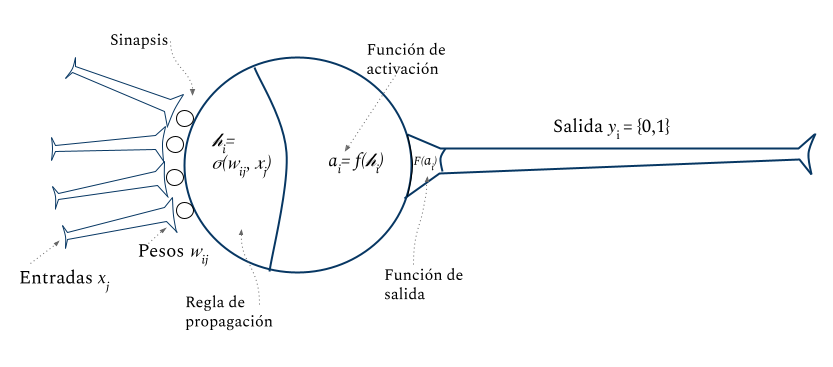
\includegraphics[scale=0.5]{../Figuras/Percp.png}
 \caption{Neurona vista como un modelo artificial (perceptrón).}
 \label{fig:unaNeurona}
\end{figure}


Un perceptrón toma un vector de entradas de numeros reales, calcula una combinación lineal de estas entradas, luego emite un 1 si el resultado es mayor que algún umbral y -1 de lo contrario. 
Es decir, dadas las entradas $x_{1}... x_{n}$, la salida $o(x_{1}. ..., x_{n})$ calculada por el perceptrón es 1 si $w_{0} + w_{1}x_{1} + w_{2}x_{2} + ... + w_{n}x_{2} > 0 $ y -1 de lo contrario, donde cada $w$ es una constante $\mathbb{R}$, un peso, que determina la contribución de la entrada $x$ a la salida del perceptrón.  La constante $w_{0}$ es un \emph{umbral} (bias) que la suma de las entradas con los pesos debe superar para que el perceptrón emita un 1. En otras palabras es un peso que va a actuar junto con una entrada de valor $1$, que vamos a poder ajustar para que nuestrá función de activación, se mueva de derecha a izquierda en el plano para ayudarnos a ajustar nuestros resultados, provocando un gran impacto en el aprendizaje. Esto se muestra en la siguientes graficas \ref{fig:bias}. Más adelante hablaremos de su regla de entrenamiento (Training rule).

\begin{figure}[h]
    %\centering
    \subfloat[Función sigmoide.]{
            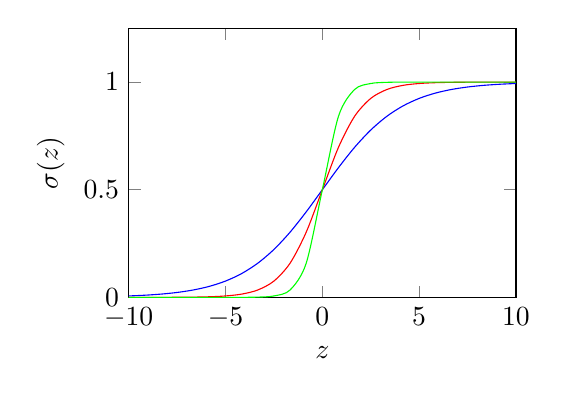
\begin{tikzpicture}
            \begin{axis}[width=6.5cm,height=5cm,ylabel=$\sigma(z)$,xlabel=$z$,ymin=0,ymax=1.25,xmin=-10,xmax=10]
                \addplot[domain=-10:10,blue,smooth] {1/(1+exp(-(x*.5)))};
                \addplot[domain=-10:10,red,smooth] {1/(1+exp(-(x* 1)))};
                \addplot[domain=-10:10,green,smooth] {1/(1+exp(-(x* 2)))};
                %\addlegendentry{$y = \dfrac{1}{1+e^{-x}}$}
            \end{axis}
        \end{tikzpicture}
    }
    \subfloat[Función sigmoide con bias.]{
            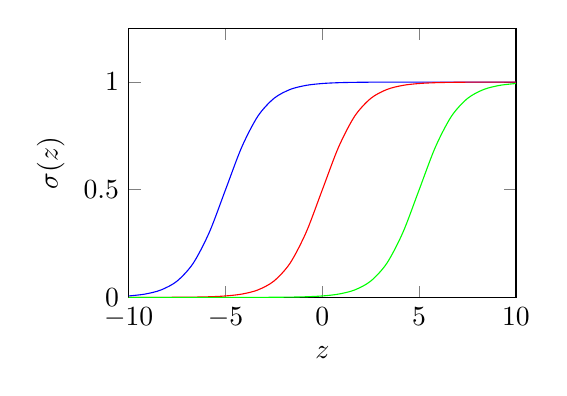
\begin{tikzpicture}
            \begin{axis}[width=6.5cm,height=5cm,ylabel=$\sigma(z)$,xlabel=$z$,ymin=0,ymax=1.25,xmin=-10,xmax=10]
                \addplot[domain=-10:10, blue,smooth] {1/(1+exp(-(x*1 + 5)))};
                \addplot[domain=-10:10, red,smooth] {1/(1+exp(-(x* 1)))};
                \addplot[domain=-10:10, green,smooth] {1/(1+exp(-(x* 1 - 5)))};

                %\addlegendentry{$w = -5$}
            \end{axis}
        \end{tikzpicture}
    \label{fig:bias}
    }
    \caption[Impacto del bias]{
     Comportamiento de la función de activación (sigmoide) de un perceptrón con una sola entrada, \emph{(b)} el perceptrón sin el uso de bias, \emph{(b)} con el uso del bias, donde apesar de estár representandos con la misma entrada , el uso del bias afecta en los resultados de salida. Así si quisieramos que este perceptrón nos diera $y = 0$ con una entrada $x= 2$ sin el uso, ni ajuste del bias sería imposible, pues en (a) apesar que la gráfica azul está la entrada está ajustada con el peso $w=0.5$, la roja con el $w=1$, y la verde con el $w=2$  solo lo gramos alargarla un poco, haciendo que entradas que antes eran correctas ahora caigan $0$ también. Entonces lo que necesitamos es más bien "mover" la gráfica, esto lo logramos con la gráfica \emph{(b)} donde la entrada (única) está sumada con un bias (umbral) $x_{0}= 1$, ajustado en azul con peso $w_{0}= 5$, en rojo con $w_{0}= 0$, en verde con $w_{0}= -5$ y el peso $w_{1}=1$. Donde con $w_{0}= -5$ logramos nuestro objetivo de tener una salida $y=0$ con $x=2$. El bias nos permite mover la función fuera del origen.
     \label{fig:sigmoideBias}
     }
\end{figure}


El hecho de que un perceptrón aprenda implica elegir valores para los pesos denotados también por $\theta$.  Ahora, el espacio $H$ de las hipótesis candidatas consideradas en el aprendizaje del perceptrón, es el conjunto de todos los posibles vectores de pesos.  \[H = {\vec{w} |  \vec{w} \in \mathbb{R}^{n+1}}\].

\begin{figure}[h]
 \centering
 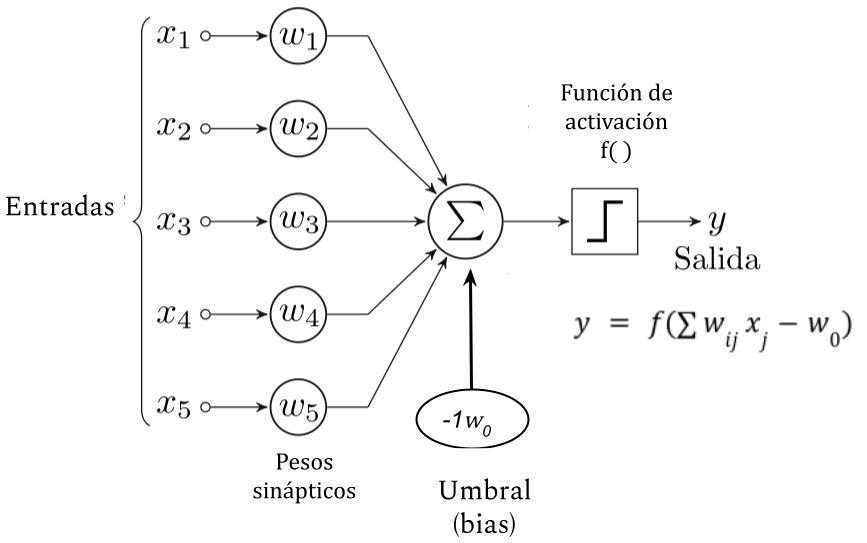
\includegraphics[scale=0.5]{../Figuras/Perceptron.png}
 \caption{Modelo estandar de un perceptrón.}
 \label{fig:unaNeurona2}
\end{figure}

Si bien en el momento que se publicó los logros con el modelo del percetrón las espectativas eran bastante altas, a medida de los años los cientificos Marvin Minsky and Seymour Papert desestiman en gran medida los alcances que realmente se puede tener con el perceptrón, al mostrar \footnote{ En 1969 publican Marvin Minsky y Seymour Papert que perceptrones de una sola capa (simples) solo son capaces de aprender a distinguir patrones linealmente separables, en el libro "Perceptrons".
} que no puede predecir operaciones lógicas que no sean linealmente separables, tal es el caso de la función XOR, que no es separable linealmente, siendo imposible que pueda aprender está función. Esto y el gran costo que representaba procesar todos los elementos que implicaba el entrenamiento, causa que por un buen tiempo se desetime el uso del perceptrón. Es hasta después de unas decadas que vuelve a tener relevancia con la propuesta de un perceptrón multicapa usando retropagación (Feedforward), siendo estos capaces de resolver la función XOR



\section{Compuertas lógicas con neuronas}
%operaciones lógicas

Aquí se muestra como se puede utilizar un perceptrón para simular compuertas lógicas tales como el or, not, and.

Para simular la compuerta \emph{not}, como está es una función boolean de \(B \rightarrow  B\), talque $not(x) = -x$ entonces en un plano de dos dimensiones, la podemos representar con dos puntos, el  $p_{1} = (0,0)$  y $p_{2} = (1,0)$donde $p_{1}$ representa cuando $not(0) = 1$, $p_{1}$ representa cuando $not(0) = 1$. Teniendo el espacio de la función definido lo que nos toca es, separar el plano para clasificar las entradas, este claramente se puede separar con un linea vertical, o con lineas con pendiente $1$ o $-1$. Para esta función solo necesitamos de una entrada y un sesgo (bias), donde la entrada la combinaremos con un peso, este peso lo asignaremos a tanteo (por la sencillez de la operación). Así el peso $w_{1} = -1$  y el peso asignado al bias sera $w_{0} = 0.5$, ahora con esto datos podemos:

\begin{itemize}
 \item Hacer la función de propagación donde $h(x) =  (x * -1) + (0.5) * 1 = 0.5 - x$
 \item Haccer la función de activación escalón $a(x) = sgn(h) = sgn(0.5-x)$ 
 \item Dar la salida donde $s(1) = sgn(0.5-1) = 0$ y $s(0) = sgn(0.5-0) =  1$, en este caso la salida es la identidad de la activación.
\end{itemize}

\begin{table}[H]
 \centering
\begin{tabular}{ | c | c |c | } 
 \hline
 $x$ &  $h$ & $s$ \\
 \hline
 $0$ &  $0.5$ & $1$ \\
 \hline
 $1$ &  $-1.5$ & $0$ \\
\hline
\end{tabular}
 
\end{table}


Algo similar va a pasar con la compuerta \emph{and} y \emph{or} donde al necesitar de dos entradas para la compuerta, asignaremos dos entradas para el perceptrón igualmente y las representaremos en el plano con cuatro puntos, donde cada punto representa una instancia y se le asigna valor positivo o negativo en el plano, así pues para el and tenemos los puntos $p_{1} = (0,0)$, $p_{2} = (0,1)$ , $p_{3} = (1,0)$, negativos y $p_{4} = (1,1)$ el único positivo. Así nos damos cuenta que necesitamos una recta con pendiente negativa y fuera del origen, que nos separe estás clases de puntos. Por tanto para el bias le asignamos un peso de $w_{0} = -1.5$, $w_{1} = 1$ y $w_{2} = 1$, con estos datos podemos: 


\begin{itemize}
 \item Hacer la función de propagación donde $h((x_{1},x_{2})) =  (x_{1} * 1) + (x_{2} *1) + (-1.5) * 1 = x_{1} + x_{2} - 1.5$
 \item Haccer la función de activación escalón $a((x_{1},x_{2})) = sgn(h) = sgn(x_{1} + x_{2} - 1.5)$ 
 \item Dar la salida donde $s = a(\vec{x})$, es la identidad de la activación.
\end{itemize}

\begin{table}[H]
 \centering
\begin{tabular}{ | c | c| c |c | } 
 \hline
 $x_{1}$ & $x_{2}$ & $h$ & $s$ \\
 \hline
 $0$ & $0$ & $-1.5$ & $0$ \\
 \hline
 $0$ & $1$ & $-0.5$ & $0$ \\
 \hline
 $1$ & $0$ & $-0.5$ & $0$ \\
 \hline
 $1$ & $1$ & $0.5$ & $1$ \\
\hline
\end{tabular}
 
\end{table}


Para la compuerta \emph{or} es algo muy similar pues podemos igualmente representar la función con cuatro puntos en el espacio cada uno representando una instancia, solo que ahora tres de estos puntos serán positivos y solo uno negativo, los puentos positivos serían $p_{2} = (0,1)$ , $p_{3} = (1,0)$ y $p_{4} = (1,1)$, mientras que $p_{1} = (0,0)$ negativo, el plano lo podemos dividir con una linea recta con pendiente negativa, así le asignamos $w_{0} = - 0.5$, $w_{1} = 1$ y $w_{2} = 1$, con esto hacemos los paso que ya sabemos:

\begin{itemize}
 \item Hacer la función de propagación donde $h((x_{1},x_{2})) = (x_{1} * 1) + (x_{2} *1) + (-0.5) * 1 = x_{1} + x_{2} + 0.5$
 \item Haccer la función de activación escalón $a((x_{1},x_{2})) = sgn(h) = sgn(x_{1} + x_{2} + -0.5)$ 
 \item Dar la salida donde $s = a(\vec{x})$, es la identidad de la activación.
\end{itemize}

\begin{table}[H]
 \centering
\begin{tabular}{ | c | c| c |c | } 
 \hline
 $x_{1}$ & $x_{2}$ & $h$ & $s$ \\
 \hline
 $0$ & $0$ & $-0.5$ & $0$ \\
 \hline
 $0$ & $1$ & $0.5$ & $1$ \\
 \hline
 $1$ & $0$ & $0.5$ & $1$ \\
 \hline
 $1$ & $1$ & $-1.5$ & $1$ \\
\hline
\end{tabular}
 
\end{table}


Tomando el hecho que en la naturaleza las neuronas van pasando información en una estructura que forma niveles de abstración, esto lo modelamos como capas de neuronas conectadas entre sí, cada capa haciendo su trabajo de abstración.
El perceptrón simple es un modelo neuronal unidireccional, una capa de entrada y otra de salida, que por si solo no puede separar todas la funciones lógicas pues tenermos el XOR, para resolver esto usaron perceptrones multicapa que se explicará más adelante en el curso.  

\section{Funciones de activación}

Recordando que la forma de las funciones de activación es $y = f(x)$, donde $x$ representa el potencial postsináptico e $y$ el estado de activación de la neurona, es decir si va a lanzar un disparo o no. Las funciones de activación más empleadas son:

\begin{figure}[h]
    \centering
    \subfloat[Función logistica.]{
            \begin{tikzpicture}
            \begin{axis}[width=5.5cm,height=4cm,ylabel=$\sigma(z)$,xlabel=$z$,ymin=0,ymax=1.25,xmin=-5,xmax=5]
                \addplot[blue,smooth] {1/(1+exp(-x))};
                \addlegendentry{$y = \dfrac{1}{1+e^{-x}}$}
            \end{axis}
        \end{tikzpicture}
    }
    \subfloat[Función tangente hiperbólica.]{
        \begin{tikzpicture}
            \begin{axis}[width=5.5cm,height=4cm,ylabel=$\tanh(z)$,xlabel=$z$,ymin=-1.25,ymax=1.25,xmin=-5,xmax=5]
                \addplot[blue,smooth] {tanh(x)};
                \addlegendentry{$y = \dfrac{e^{x}-e^{-x}}{e^{x}+e^{-x}}$}
            \end{axis}
        \end{tikzpicture}
    }\\
    \subfloat[Función escalón.]{
            \begin{tikzpicture}
            \begin{axis}[width=5.5cm,height=4cm,ylabel=$\sigma(z)$,xlabel=$z$,ymin=-0.1,ymax=1.25,xmin=-1,xmax=1]
                \addlegendimage{ultra thick,blue}
                \addplot[ultra thick,blue,mark=*,mark options={fill=white},samples at={-1.1,0}] {0};
                \addplot[ultra thick,blue,mark=*,samples at={0,1.1}] {0.5};
                \addlegendentry{$y=\begin{cases} 1 \quad &\text{si} \, x \geq 0 \\ 0 \quad &\text{si} \, x < 0 \\ \end{cases}$
            }   
            \end{axis}
        \end{tikzpicture}
    }
    \subfloat[Función lineal a tramos. Tangente hiperbólica rectificada.]{
        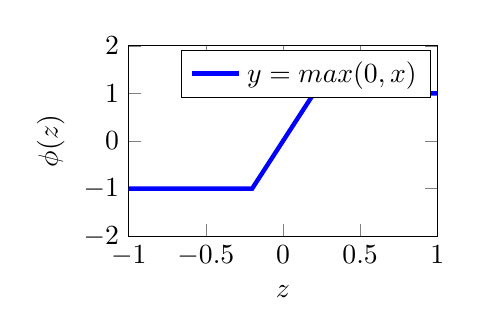
\begin{tikzpicture}
            \begin{axis}[width=5.5cm,height=4cm,ylabel=$\phi(z)$,xlabel=$z$,ymin=-2,ymax=2,xmin=-1,xmax=1]
                \addplot[blue,ultra thick] coordinates {(-1.1,-1) (-0.2,-1) (0.2,1) (1.1,1)};
                \addlegendentry{$y=max(0,x)$}
            \end{axis}
        \end{tikzpicture}
    }
        \caption[Funciones de activación sigmoides]{
        Las funciones de activación más usadas son la función sigmoide $\sigma(z)$ y la tangente hiperbólica $tanh(z)$.}
        \label{fig:sigmoid-tanh}
\end{figure}



\section{Funciones de error}

Entonces tomando como base el perceptrón, una vez obtenidas las salidas con una primera iteración nos daremos cuenta de que tan lejos o que tan cerca estuvimos de la respuesta correcta, con esto darnos la oportunidad de que pesos ajustar respecto a sus entradas, en la segunda iteración. Ahora para facilitarnos esto y tomando en cuenta que el entrenamiento consiste en varias iteraciones hasta llegar a aprender la tarea T, hacemos uso de una función de error que nos ayude a minimizar la diferencia de error en las salidas. 

Primero veamos el entrenamiento para una sola neurona, para esto haremos uso de la regla de aprendizaje del perceptrón (learning rule perceptron), donde para cada entrada, en la capa de salida se le calcula la desviación a la función objetivo. El cual utilizamos para ajustar los pesos del perceptrón (ver fig \ref{fig:errorP}). 

\begin{figure}[h]
 \centering
 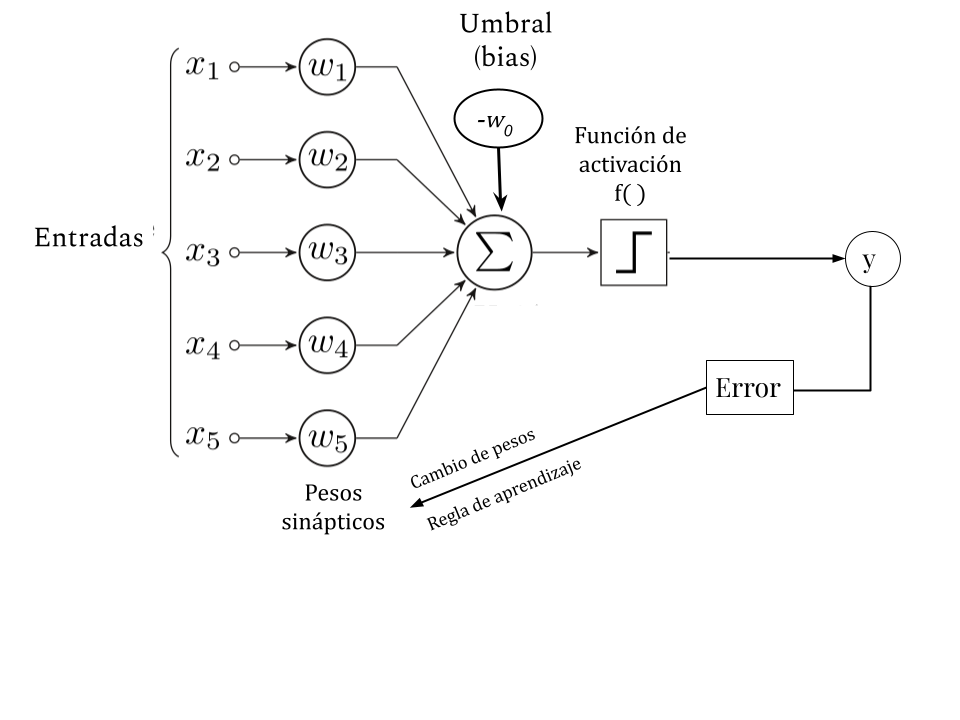
\includegraphics[scale=0.5]{../Figuras/ErrorPerceptron.png}
 \caption{Modelo estandar de un perceptrón.}
 \label{fig:errorP}
\end{figure}

Usualmente al principio del entrenamiento se asignan pesos aleatorios, a medida que avance el entrenamiento, se van modificando con cada iteración, así \(w_{i} \leftarrow w_{i} + \Delta w_{i}\). Esto con base a \emph{la regla de aprendizaje} donde: 

\begin{equation}
 \Delta w_{i} = \alpha(y - y_{out})x_{i}
\end{equation}

 
Con $y$ es la salida deseada, $y_{out}$ la salida generada, $\aloha$ la taza de aprendizaje (learning rate) y $x_{i}$ la entrada $i$. Lo que hace la taza de aprendizaje es moderar el grado en que los pesos son cambiados con cada iteración, se le asigna un valor muy pequeño (0.1 o 0.2) y conforme se logran ajustar los pesos se minimiza aún más. 


%Ahora supongamos que logramos que el perceptrón aprenda los datos
% de entrada, esto nos indica que $y = y_{out}$, haciendo que \
%(\Delta w_{i} = 0\), por tanto, ningún peso se actualice. En %nuestra etapa de validación, en un ejemplar nos de la salida $y = %-1$, cuando lo indicado es $1$. Entonces seguido de esa prueba %necesitamos hacer cambio de la taza de aprendizaje y renovación de %pesos aleatorios, para volver a ajustar los pesos correctamente y %no quede sobreajustada.


Para entrenar un perceptrón, utilizamos cualquier método de optimización de funciones para encontrar los parámetros $w$ que minimizan el error con alguna de las siguientes funciones de error:

\begin{description}
   
 \item \textbf{Diferencias al cuadrado}, también conocida como regla aprendizaje delta, es la suma de cuadrados de errores que se tuvieron con cada ejemplar el el conjunto de entranamiento. Los podemos decribir como: 
 
 \begin{equation}
   \dfrac{1}{2m}\sum_{m=0}^{M-1} (y_{m} - a_{m})^2
 \end{equation}
 
 con $y_{m}$ y $a{m}$, la salida obtenida dado un ejemplar $m$ y la salida correcta del ejemplar $m$ respectivamente.
 
 \item \textbf{Entropía cruzada.} Se usa para problemas de clasificación ya que su comportamiento es más suave (soft) y permite hacer clasificaciones más certeras. Se define como:

 \begin{equation}
  L (\Theta) = -\dfrac{1}{m}\sum_{M-1}^{m=0}(y^(m)log(a_{m}) + (1-y_{m}) log(1-a_{m})) 
 \end{equation}

\end{description}

Entonces juntando los conceptos que ya sabemos podemos describir el algoritmo de entrenamiento para el perceptrón de la siguiente forma:
\begin{enumerate}
 \item Iteramos sobre todos los ejemplares.
 \item Para cada ejemplar se calcula la función de propagación, es decir la suma ponderada.
 \item Se calcula la función de activación con esta suma.
 \item Se calcula la función de salida.
 \item Actualización de pesos de acuerdo a la regla de aprendizaje.
 \item Repetir de 1-6 hasta que los pesos nos satisfagan, un número de iteraciones establecidas.
\end{enumerate}


%Viéndolo como una especie de pseudocódigo lo podemos ver como:

%\begin{verbatim}
% Perceptron
%	input: Ejemplares
%	w: Pesos
%	y: correctas	
%	ta: taza de aprendizaje
%	o: respuestas predichas
%	
%Entrenamiento (input, w, y, ta):
%
%	for m in input: #iteramos sobre cada ejemplar
%		h = sum (w[m] * input[m]) #regla de propagación 
%		a = funcionActivacion(h) 
%		o[m] = 1 if (a*y[m]) > 0 else 0 #función de salida
%		w[m] = w[m] + (y[m] - o[m]) * ta * input[m] #regla de aprendizaje.
%
%\end{verbatim}



\section{Medidas de rendimiento}

Las medidas de rendimiento de una red nos sirven para ver de manera croncreta como se comportó nuestra red, durante el entrenamiento, que fue lo que pudo aprender, que sobre aprendio, es decir, memorizo, y que aún le cuesta trabajo aprender, por tanto, será incapaz de predecir. Se usan las siguientes:

\begin{description}
 \item [Matriz de confusión]: (Confusion matrix)
 Es una matriz, donde las celdas representan las predicciones que hizo nuestro modelo de clasificación de clases, respecto a las salidas esperadas. Así siendo las columnas las salidas $y$'s del modelo entrenado y las filas las salidas esperadas $y_{true}$. 
 Nos facilita a ver cuando un clasificador está confundiendo clases, contabilizando a que clase etiqueto a los diferentes ejemplares. Ahora veamos, que puede estar representando cada celda en la matriz de confusión, estos pueden ser:
 \begin{enumerate}
  \item \textbf{VP} Verdaderos positivos \emph{(TP, True Positive)}: La clasificación de los ejemplares predichos, condicen con las etiquetas esperadas de los ejemplares. 
  
  \item \textbf{VN} Verdaderos negativos \emph{(TN, True Negative)}: El ejemplar que no es parte de clase, no son asignados a esa clase, son predichos correctamente.
  
  \item \textbf{FP} Falso positivo \emph{(FP, False Positivo)}: El ejemplar que \textbf{no} es parte de una clase $i$ fue clasificado como tal.
  
  \item \textbf{FN} False negativo  \emph{(FN, False Negative)}: El ejemplar que es parte de una clase $i$ no fue clasificado como tal. 
 \end{enumerate}

  \begin{example}
   Notemos un ejemplo sencillo, supongamos que tenemos una tarea binaria, donde queremos indicar que una persona está
   embarazada (de acuerdo a unos estudios). Ahora tenemos que:
   

   \begin{itemize}
    \item \emph{VP}, sería predecir que una mujer está embarazada y que en efecto esté embarazada. \textbf{(Correcto)}
    \item \emph{VN}, sería con un hombre que no está embarazado y pues en efecto no está embarazado.\textbf{(Correcto)}  
    \item \emph{FP}, sería predecir que un hombre está embarazado y \textbf{no} este embarazado. \textbf{(Error, tipo 1)} 
    \item \emph{FN}, sería predecir que una mujer \textbf{no} está embarazada y esta embarazada. \textbf{(Error, tipo 2)}
   \end{itemize}


   Entonces dados los resultados binarios que nos entregó el modelo, los médicos nos dan las respuestas correctas a 10
   estudios, representadas en la siguiente tabla.
 
   \begin{center}
    \rowcolors{2}{\colTableRow}{white}
     \begin{tabular}{c|cccccccccc}

      $Ejemplar$ & 1   & 2  & 3  & 4  & 5  & 6  & 7  & 8  & 9  & 10  \\ \hline
      $Sujeto$   & M   & F  & M  & F  & M  & M  & F  & F  & F  & M  \\ \hline
      $Etiqueta$ & No  & Si & No & Si & No & No & No & Si & No & No  \\ \hline
      $Clase$    & 0   & 1  & 0  & 1  & 0  & 0  & 0  & 1  & 0  & 0  \\ \hline
      $Predicho$ & 0   & 0  & 0  & 1  & 0  & 1  & 0  & 1  & 0  & 0  \\ \hline
      $Valores$  & VN  & FN & VN & VP & VN & FP & VN & VP & VN & VN  \\ \hline
   
     \end{tabular}
   \end{center}

   Con estos datos, podemos construir nuestra matriz de confusión $MC$ contabilizando las salidas obtenidas respecto a las deseadas. Quedando así de la siguiente manera:

   \begin{table}[H]
    \begin{center}
     \begin{tabular}{|c|c|c|c|}
     \cline{3-4}
     \multicolumn{2}{c|}{} & \multicolumn{2}{c|}{Salidas $y$} \\
     \cline{3-4}
     \multicolumn{2}{c|}{} & Si & No \\
     \hline
     \multirow{3}{*}{Etiquetas} & Si & $VP = 2$ & $FN = 1$ \\
     \cline{2-4}
     & No & $FP=1$ & $VN = 6$  \\
     \hline
     \end{tabular}
    \end{center}
    \caption{Matriz de confusión binaria.}
    \label{Table2}
   \end{table}

\label{ej:binario}
\end{example}
 
 
 Ahora para una modelo que sea multiclase, en el que tengamos que clasificar varias clases de ejemplares. Tendremos una matriz $M$ de $n * n$ donde $n$ es el número de clases, así los valores \emph{VP, VN, FP, FN}, son calculados para cada clase e identificados en la matriz $M$ de la siguiente forma, también puedes ver la figura \ref{fig:mcMult}:
 \begin{itemize}
  \item \emph{VP}, para la clase $i$ será la celda $M[i][j]$ con la $i = j$.
  
  \item \emph{VN}, para la clase $i$ será la suma de los valores de toda la matriz menos los valores de la fila $i$ ni los valores de la columna $i$. 
  
  \item \emph{FN}, para la clase $i$ será la suma de los valores en la fila $i$, excepto la celda $M[i][j]$, con $i=j$ que es el \emph{VP}.
  
  \item \emph{FP}, para la clase $i$ será la suma de los valores en la columna $i$, excepto la celda $M[i][i]$ que es el \emph{VP}.
 
 \end{itemize}
 
  \begin{figure}[H]
 \centering
 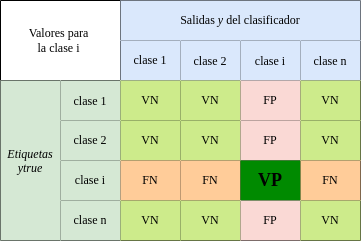
\includegraphics[scale=0.7]{../Figuras/MC_multiple.png}
 \caption{Matriz de confunsión para clasificador multiclases.}
 \label{fig:mcMult} 
\end{figure}

 
 \begin{example}
Tenemos un clasificador encargado de identificar las cinco vocales del español, escritas a mano. Entonces tenemos un total de 5 clases representadas por $a, e, i, o, u$, cada letra representada por un número del 0 al 4. Así la clase $0 = a$, la clase $1 = e$ y así respectivamente. Este fue entrenado con 15 ejemplares etiquetados y se obtuvieron los siguientes resultados:


\begin{center}
\rowcolors{2}{\colTableRow}{white}
\begin{tabular}{c|ccccccccccccccc}

 $Ejemplar$ $e$     & 1 & 2 & 3 & 4 & 5 & 6 & 7 & 8 & 9 & 10 & 11 & 12 & 13 & 14 & 15 \\ \hline
 $Etiqueta $      & a & e & i & o & u & a & a & e & i & i  & o  & u  & o  & u & a \\ \hline
 $Clase$ $y_{true}$ & 0 & 1 & 2 & 3 & 4 & 0 & 0 & 1 & 2 & 2  & 3  & 4  & 3  & 4 & 0 \\ \hline
 $Predicho$ $y$     & 0 & 1 & 3 & 3 & 2 & 1 & 1 & 1 & 2 & 2  & 4  & 4  & 3  & 2 & 0 \\ \hline

\end{tabular}
\end{center}

 Ahora para hacer la matriz de confusión $MC$ notamos que tenemos una matriz de $5 x 5$, donde $MC[i]= Predicho$ y $MC[][j] = EtiquetasReales$. Entonces necesitamos contabilizar las predicciones y asignarlas a sus respectivas celdas, donde con la tabla anterior notamos que en el ejemplar $e3$ con $y_{true}(e3)= 2$, se predijo que $y(e3)=3$, entonces $MC[2][3] +=1$, pues la etiqueta nos posiciona en la fila $2$ y lo predicho en la columna $3$. Ahora en el ejemplar $e4$ con $y_{true}(e4)= 3$ se predijo que $y(e4)= 3$, entonces  $MC[2][2] +=1$. Así con cada ejemplar vamos a ir sumando su clasificación. Para construirla tendríamos un pseudocódigo siguiente:
 \begin{verbatim}
  def getMC (Ejemplares, y):
      """
      :param y:  salidas obtenidas (int)
      """
      MC = [len(y)][len(Ejemplares] # y == Ejemplares
      full_zeros(MC)
      for e in range (0, len(Ejemplares)):
          predicho = y[e]
          y_true = Ejemplares[e].etiqueta
          MC[predicho][y_true] += 1
  retrun MC
 \end{verbatim}

Dados los datos anteriores tenemos, la siguiente matriz de confusión: 
 \begin{table}[H]
\begin{center}
%\rowcolors{2}{\colTableRow}{white}
\begin{tabular}{|c|c|c|c|c|c|c|c|}
\cline{3-8}
\multicolumn{2}{c|}{} & \multicolumn{5}{c|}{Salidas $y$} \\
\cline{3-8}
\multicolumn{2}{c|}{} & 1 & 2 & 3 & 4 & 5 \\
\hline
\multirow{5}{*}{\begin{sideways} Etiquetas~ \end{sideways}} & 1 & $2$ & $2$ & $0$ & $0$ & $0$ \\
\cline{2-8}
& 2 & $0$ & $2$  & $0$ & $0$ & $0$ \\
\cline{2-8}
& 3 & $0$ & $0$  & $2$ & $1$ & $0$ \\
\cline{2-8}
& 4 & $0$ & $0$  & $0$ & $2$ & $1$ \\
\cline{2-8}
& 5 & $0$ & $0$  & $2$ & $0$ & $1$ \\
\hline
\end{tabular}
\end{center}
\caption{MC = Matriz de confusión multiclase.}
\label{Table2}
\end{table}

\label{ej:muticlase}
\end{example}
 

 Para calcular los valores \emph{VP, VN, FP,FN}, por clase se propone el siguiente pseudocódigo:
 \begin{verbatim}
  MC = getMC(y_salidas, y_true)
  
  VP = VN = FP = FN = [0,0,0,0,0]

  for i in range(len(MC)):
    for j in range(len(MC[0])):
        FN[i] = FN[i] + MC[i][j] if (i != j) else FN[i]
        FP[i] = FP[i] + MC[j][i] if (i != j) else FP[i]
        VP[i] = MC[i][j] if (i == j) else VP[i]
    VN[i] = sum(MC) - FN[i] - FP[i] -VP[i]
 \end{verbatim}

 Si quisiéramos saber los valores \emph{VP, VN, FP,FN}, para todo el desempeño total, simplemente sumamos lo obtenido en cada clase así:

 \begin{verbatim}
  VP_total = sum(VP)
  VN_total = sum(VN)
  FP_total = sum(FP)
  FN_total = sum(FN)
 \end{verbatim}

    Ahora los valores de cada celda nos representan lo siguiente:
 
   \begin{itemize}
     \item \emph{$VP_{total}$}, toda la diagonal de la matriz. La salida del modelo coincide con lo etiquetado con el ejemplar.
     \item \emph{$VN_{total}$}, todas las veces que no era la clase i y dijo que no era de la clase i.
     \item \emph{$FN_{total}$}, todas las veces que era $clase_{i}$ y dijo que era $clase_{x}$. (deseado $FN = 0$ )
     \item \emph{$FP_{total}$}, todas las veces que predijo que era $clase_{i}$ y era $clase_{x}$. (deseado $FP = 0$ )
   \end{itemize}
 
    Así que, si los valores que no están en la diagonal de la matriz son cero o todas nuestras clasificaciones están en la diagonal, podemos decir que nuestro modelo aprendió a clasificar correctamente todas las clases.
 
 \end{description}
\begin{description}

 \item [Precisión y recuperación]: 
 La precisión (\emph{precision}) nos dice la proporción de ejemplares que se logró clasificar correctamente. 
 Mientras que recuperación (\emph{recall}) nos dice cuantas asignaciones de lo que nos interesa pudo clasificar correctamente en otras palabras donde del total de las respuestas correctas que se pueden tener, cuantas respuestas positivas acertadas se tuvo.
 
 
    \begin{equation}
        P = \dfrac{VP}{VP + FP}  = \dfrac{Verdaderos Positivos}{Valores Esperados}
    \end{equation}
    \begin{equation}
        R = \dfrac{VP}{VP + FN} = \dfrac{Verdaderos Positivos}{Valores Predichos}
    \end{equation}

    \begin{figure}[H]
        \centering
        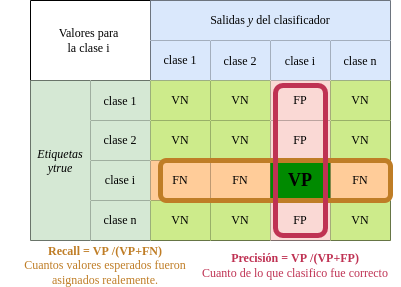
\includegraphics[scale=0.7]{../Figuras/Medidas_pr.png}
        %\caption{Matriz de confunsión para clasificador multiclases.}
     \label{fig:mcPR} 
    \end{figure}

    
    \begin{itemize}
     \item Cuando el modelo detecta los ejemplares, pero los incluye en otras clases también: \emph{P} es bajo y \emph{R} es alto. 
     \item Cuando el modelo no detectó bien los ejemplares, pero tampoco los incluyo en otras clases: \emph{P} es alto y \emph{R} es bajo. 
     \item Cuando el modelo detecta los ejemplares y no los incluye en otras clases:\emph{P} y \emph{R} es alto. 
     \item Cuando el modelo no detecta los ejemplares:\emph{P} y \emph{R} es bajo. 
     \end{itemize}


     En ocasiones le daremos más importancia al recall y en otras a la precisión. Retomando el ejemplo previo \ref{ej:binario}, no nos importa tanto los casos de error tipo 1, donde el modelo se equivoco con los ejemplares negativos, nos importa los errores de tipo 2, los Falsos Negativos, en este caso le tomaremos especial atención al Recall y que este sea alto. Pero si bien nuestra tarea es detectar cuando un correo es spam, no impacta tanto que aunque en ocasiones un correo sea spam, no lo clasifique como tal (error tipo 2 FN), nos es crucial que un correo que no sea spam nos lo clasifique como tal (error tipo 1 FP). Así deseando que los falsos positivos se acerquen a cero, dándonos como resultado una precisión alta aunque el recall sea bajo. 

     
 \item [Exactitud y medida f ]: La exactitud (\emph{accurrancy}) es una medida de cuántas predicciones correctas en total hizo el modelo para el conjunto de datos completo (no se recomienda usar si tienes clases desbalanceadas, es decir, muchos elementos de una clase y poco de otra pues nos puede fallar totalmente con las clases pequeñas y aun así su valor sería alto). La medida f (\emph{(f score)}) se utiliza para combinar las medidas de precisión y recall en un solo valor. Es práctico porque hace más fácil el poder comparar el rendimiento combinado de la precisión y la recall. Se dan las ecuaciones a continuación:
    
    \begin{equation}
     Acurrancy = A = \dfrac{VP+VN}{VP + VN + FP + FN} = \dfrac{VP+VN}{Todos Los Valores Clasificados}     
    \end{equation}

    \begin{equation}
     F = \dfrac{2}{\dfrac{1}{P} +\dfrac{1}{R} }= 2 \dfrac{P * R}{P + R}
    \end{equation}

La medida f, también la podemos escribir (con un poco de aritmética) como:
    \begin{equation}
     F = \dfrac{2VP}{2VP+FP+FN}
    \end{equation}




\chapter{Perceptrón multicapa}
\section{Intro}

Perdí el archivo :CCCC

\section{XOR}


Anteriormente, habíamos logrado separar clases de ejemplares siempre y cuando estos se pudieran modelar en un plano linealmente separable. Hasta ahora había sido un reto importante (no logrado) hacer clasificaciones de ejemplares distribuidos en un plano no separable linealmente, como lo es \emph{la función XOR} donde, tenemos que las respuestas positivas se encuentran en una diagonal opuesta a las respuestas negativas y no hay manera de separar a los blancos de los negros con una sola frontera lineal, lo que hace imposible separar con un solo perceptrón. Entonces notamos que necesitamos de dos líneas que nos permitan separar el plano. Así llegamos a la idea que necesitamos más de una capa, que nos permita hacer la siguiente separación del plano.


(Insertar imágenes de la función XOR y su plano).


En la tabla de verdad notamos que para la función XOR, cuando la suma de las entradas es:
\begin{itemize}
 \item par (tomando en cuanta al cero como par) la salida es $0$.
 \item impar la salida es $1$.
\end{itemize}


Para poder aprender la función únicamente tenemos que añadir una capa intermedia, la llamada capa oculta. Esta capa será la responsable de tomar las características de los vectores de entrada.


Ahora para la función tenemos dos entradas, una capa oculta (con dos neuronas) y una salida. Las neuronas en la capa oculta nos permitirán dividir el plano. Así, una solución sería que las neuronas ocultas denotadas por $h$ (\emph{hidden} de oculto en inglés) compartan pesos, la primera neurona $h_1$ haría la función $OR$, haciendo la distinción entre las entradas $0 0$, la segunda neurona $h_2$ haría la función $NAND$ haciendo posible distinguir el vector de entrada $1 1$, una vez obtenido estos resultados de la capa oculta la neurona de salida $o$ de output se encargara de distinguir la intersección entra estas, ejecutando la función $AND$. En resumen, la función \emph{XOR} la podemos rescribir como:


\begin{equation}
 \begin{split}
    XOR &= (x_{1} \vee x_{2}) \wedge \neg(x_{1} \wedge x_{2}) \\
    XOR &= AND (OR(x_{1}, x_{2}), NAND(x_{1}, x_{2}))
 \end{split}
\end{equation}







\section{Propagación hacia adelante manual}

En está parte vamos a ver como podemos evaluar la red para la solución que se dio en la sección anterior. (Recordemos que tambíen se pueden dar otras soluciones para el XOR).

Entonces el procedimiento matemático general para poder evaluar una red cuando tenemos más de un perceptron. Veamos primero que pasa con el \textbf{xor}, y el \textbf{nand}, por el momento no tomaremos en cuenta las neuronas de entrada $a$ puesto que solo son usadas para almacenar las entradas. La capa oculta está formada realmente por dos percetrones, que dan su salida a una neurona más que es la capa de salida de nuestra red. Para calcular sus salidas debemos aplicar la suma ponderada de las entradas a una función activación, así podemos ver que la salida de una neurona oculta es la siguiente:
 
\begin{equation}
 z_{j} = g (\sum_{i} w_{ij}a_i)
\end{equation}

A estos perceptrones a su vez se le estan aplicando la función de activación sigmoide:

\begin{equation}
 h_{j} = \dfrac{1}{ 1 + e^{-z}}
\end{equation}

Así la neurona de salida recibe a los perceptrones ya evaluados y listos para aplicar pesos a estos y una función de activación, que en este caso son dados de la siguiente forma:

\begin{equation}
 z_{o} = g (\sum_{j} w_{jo}h_j)
\end{equation}

\begin{equation}
 o = \dfrac{1}{1 + e ^{z_o}}
\end{equation}

Así tomando de ejemplo la función XOR, los valores de la capa oculta son evaluados de la siguiente forma, donde $x_{1}$ y $x_{2}$ son evaluados por 0 o 1 según sea necesario:

\begin{equation}
 \begin{split}
 h_{0} &= 1 \\ 
 h_{1} &= g(1w_{01} + x_{1}w_{11} + x_{2}w_{21}) \\
 h_{2} &= g(1w_{02} + x_{1}w_{12} + x_{2}w_{22}) 
 \end{split}
\end{equation}


Entonces hasta aquí ya tenemos los valores de la capa oculta, una vez que ya tenemos este conjunto de valores podemos empezar a trabajar con el tercer perceptor, sus valores de entrada van a estar dados por los valores de activación de $h1$ y $h2$ y por un  sesgo, pues recordemos que es la función $Nand$, por tanto necesitamos movernos ligeramente del origen. Lo que vamos a tener aquí la fórmula se ve similar, lo único  es que ahora los valores de entrada fueron los valores que obtuvimos en el cálculo de la capa anterior:

\begin{equation}
  o = g( h_{0}w{0o} + h_{1}w_{1o} + h_{2}w_{2o})
\end{equation}

Como estamos trabajando capa por capa, primero entran los valores con los que van a trabajar todos los perceptrones, después calculamos todos los de la capa oculta que son independientes entre sí, aunque tengan en común las mismas entradas y finalmente hacemos el caluculo de la siguiente capa, que en ese caso es la se salida, pero bien podría ser otra oculta. 

Por esto estamos hablando de un algoritmo llamado de \emph{alimentación hacia adelante}, este hay que recorrerlo de izquierda hacia derecha, para ir obteniendo los diferentes valores de activación en cada una de las capas. Una característica de este tipo de arquitectura es que, al estar las neuronas conectadas, siempre se esta conectando de las neuronas en la capa anterior hacia las neuronas en la capa siguiente. Cuando tenemos la evalucación de las capas ocultas, podemos obtener finalmente la salida final, con una evaluación final.

Si bien está forma de evalución nos lleva al resultado correcto, este metodo se puede simplificar sobretodo en el caso que estemos manejando más entradas y más perceptrones en las capas ocultas. Así nos daremos cuenta que es posible usar matrices, esta forma de evaluación la veremos en la siguiente sección.

\section{Propagación hacia adelante vectorizada (con matrices)}
Bueno sip. XD
%Propagación hacia adelante vectorizada (con matrices)
\section{Interpretación matemática del mapeo no lineal}
En esta sección vamos a ver por qué agregar una capa más nos permite calcular funciones que no era posible calcular antes es decir no basta con tener más percepciones en realidad necesitamos tener percepciones que reciban como entrada la salida de percepciones anteriores y esto lo vamos a notar aquí por eso el selector es una función tan útil para poder explicar estos conceptos de entrada que teníamos al inicio de la función sort eran los valores 0 0 0 1 1 0 y 1 1 estos solamente los podría bueno puede utilizar perceptor únicamente para evaluar funciones que sean linealmente separables entonces cuando hemos aplicado la primera capa donde pudimos poner tantas operaciones como que hicimos lo que hicimos fue tomar estas entradas y mapear las a un conjunto distinto y esté ocurriendo en este nuevo conjunto 

Observen que las entradas ahora son 01 11 11 10 es decir estas dos están duplicadas ya no tengo el 0 0 por eso es que se dice que trabajamos con un mapeo no lineal nuestra función sigmoide o nuestra función escalón transformaron nuestro espacio de manera que no tenemos ahora una relación 1 a 1 qué efecto va a tener. Aquí tenemos una vez más cuáles son las entradas originales las entradas que se obtuvieron es bueno salidas de las capas ocultas que van a hacer ahora las entradas para el último perceptor entonces veamos acá qué pasó con este cuadro aquí teníamos cuatro datos que no eran linealmente separables después de la primera capa fue como haberlo plegado a otro espacio de dos dimensiones, pero observen ahora que como que esto es bueno vamos a ver quién se mató a quién el 0 0 se convirtió en 0,1 es decir este para acá el 0,1 se convirtió en 1,1 este fue para acá el 1010 también se convirtió en 1,1 es otro de acá y el 11 se convirtió en el 10 está aquí entonces nuestros puntos negros como que giraron un poquito y quedaron aquí y nuestros dos puntos blancos quedaron mapeados uno encima del otro en el mismo punto de este lado. 

Entonces ahora sí lo puedo separar con un plano qué pasa en medio de los dos cualquiera que lo logre es bueno entonces estos tres valores quedaron mapeados ahora a un nuevo espacio que por cierto tiene una dimensión solo hay un valor. Entonces el paso fundamental radicó en que pudimos mapear este espacio hacia un espacio nuevo donde si es posible separar a nuestros datos linealmente y sobre esto pues ya simplemente aplicamos lo que podía hacer cualquier perceptual matemáticamente ese es el poder que nos está añadiendo una capa de en medio y básicamente lo podemos generalizar ahora si a cualquier función. Es posible quitar los sesgos si utilizamos la función escalón como función de activación y definimos precisamente el menor o igual para la parte del escalón en esta ocasión vamos a obtener valores que están exactamente en este punto de salto así es que vamos a tener que decir quién queda a la izquierda quien quiere a la derecha y entonces podemos hacer esto igual se necesitan dos capas, pero podemos quitarnos la parte de los sesgos porque nuestras fronteras si están pasando por ser un coma se hace solo por curiosidad bien aquí tenemos entonces ya esa interpretación vemos que los ceros negativos se van a tomar como ceros y solamente los positivos van a quedar como unos y automáticamente se puede hacer esta versión resumida. 


 %Interpretación matemática del mapeo no lineal
\section{Propagación hacia adelante multicapa}


Ahora para el modelo de una red en general tenemos otra vez nuestra nuestra arquitectura base que va a ser una red en capas también se le conoce como el perceptor multicapa en esta primera versión tenemos la capa de entrada que decíamos es la capa de chocolate porque realmente no son percepciones solamente reciben sesgos si los vamos a ocupar y nuestros datos o características para nuestros ejemplares y aquí tenemos nuestros datos de entrada esto que estamos dibujando aquí de hecho es una función una función que viene de x n y evaluado hacia digamos xy son funciones sin moldes podríamos pensar en los reales donde tendremos que llamar aquí por ejemplo m y queremos referirnos al número de neuronas en la capa de salida. 
Entonces cómo se evalúa esta función pues ingresamos nuestros datos x a la izquierda vamos propagando hacia la derecha calculando valores intermedios hasta obtener nuestra salida en tantas dimensiones como queramos tener aquí en este ejemplo por ejemplo aquí en ese día 4 aquí el 3 podría ser ahora para ir contando capas vamos a pensar que en la de entrada para hacerlo ser de la capa 0 la capa oculta le podemos llamar a 1 la siguiente capa le podemos llamar a 2 observemos entonces que es posible continuar esta definición agregando más neuronas en la parte de adelante agregando sesgos si eso es lo que queremos y agregando las conexiones correspondientes bueno nadie mucho y entonces lo único que haríamos es repetir el patrón necesitaríamos un nuevo set de conexiones entre las neuronas de la capa anterior y la siguiente y un nuevo valor de activación tantas como nosotros queramos entonces las matemáticas que vamos a plantear aquí se van a generalizar rápidamente a la inclusión de mayores capas sí sí tiene su utilidad como lo iremos viendo más adelante sin embargo también podremos ver qué para poder aproximar absolutamente cualquier función con el mapeo de aquí para acá en realidad lo único que necesitaríamos teóricamente es agregar neuronas en la capa de enmedio en teoría no necesitamos más capas adelante un poco porque va a ser necesario más adelante otras arquitecturas bueno pues porque en toda esta parte lo único que hemos visto es cómo evaluar la función que define la red neuronal si ya conocemos los pesos pero qué sucede cuando no conocemos los pesos necesitamos encontrar los pesos correctos para que esta arquitectura aproxima en la función que nosotros queremos si los tenemos que buscar entonces ahí es donde puede ser más fácil o más difícil dependiendo de la inclusión de otras capas o de otras arquitecturas entonces bueno por el momento terminemos simplemente de plantear la parte de cómo se ve la función de la red neuronal entonces decíamos el formato es vamos a hablar de los valores de activación por eso tenemos estas mayúsculas y cada una de las capas las vamos a ir numerando de izquierda a derecha después a la derecha vamos a ponerle el índice a la matriz de pesos de las conexiones que hay entre la capa anterior hacia la que vamos entonces este cero porque toma como entradas a los valores de activación cero recordemos entonces que cada uno de estos valores van a estar hechos por matrices donde las hadas pueden tener su ejemplar sobre los renglones y podríamos evaluar de una vez para varios ejemplares si los agregamos como renglones en el caso de los pesos recordemos que estamos poniendo los pesos que se conectan con cada una de las neuronas en la forma de columnas y repetimos y significa eso de que yo puedo tener a cada uno rm aquí podría querer más de una neurona vamos a definir aquí entonces un tipo de codificación que se utiliza para los problemas de clasificación y se le conoce en inglés como one hot en coding.

One hote encoding.
Falta todo esto.
 %Propagación hacia adelante para el perceptrón multicapa

%%
\chapter{Entrenamiento por retropropagación}

\section{Esquema general entrenamiento}
 
 En este capítulo vamos a trabajar con el entrenamiento (específicamente por retropropagación), en esta sección abordaremos primero el esquema general del entrenamiento. 
 A lo largo del capítulo veremos la derivación del primer algoritmo de entrenamiento para perceptrones multicapa (este es de los más comunes en esta área y el primero descrito propiamente).

En el tercer capítulo habíamos visto el concepto de aprendizaje para una máquina, ahora vamos a definir en que consiste aprender algo en el campo de las redes neuronales. Retomando lo descrito en ese capítulo, recordemos que aprender para un modelo es más que nada encontrar una función que se asemeje a ciertas salidas específicas, está función está dentro de un espacio de funciones posibles propuestas. La función que deseamos encontrar modela algún tipo de tarea que nos interesa que se aprenda. 

\begin{definition}
 \textbf{El problema de aprendizaje para un perceptrón multicapa:} Dada una arquitectura de red neuronal, encontrar los pesos tales que la función $h\Theta(\vec{x}) $ (definida por la red neuronal) aproxime, hasta cierta tolerancia, la función de interés $ f(\vec{x})$. \\ Con $\vec{x}$ los datos de entrada.
 
\end{definition}

En la definición anterior, el vector $\vec{x}$, consisten en distintas características de los ejemplares provistos, según sea el problema a resolver, por ejemplo:
\begin{itemize}
 \item Segmentos de alguna canción.
 \item Píxeles de imágenes.
 \item Valores equivalentes a precios del mercado.
\end{itemize}

En este momento nos estamos concentrando en problemas de clasificación así que estás redes estan clasificando los ejemplares según ciertas características. Estas clasificaciones pueden ser muy interesantes, algunas por ejemplo se pueden dedicar a clasificar canciones, identificando ciertas emociones que transmiten como tristeza o alegria. 

Nuestra red neuronal va empezar sus calculos apartir de los datos de entrada $\vec{x}$, entonces al finalizar cada uno de los ejemplares va a ser mapeado a alguna clase (en el espacio de clases). Por medio de una función donde $f(x)$ es nuestra función ideal que hacer el mapeo exacto los ejemplares a su clase. Así si logramos que nuestra función $h\Theta(\vec{x})$ se aproxime a $f(x)$, la red neuronal nos daría las respuestas esperadas dado ciertos ejemplares, como por ejemplo:
\begin{itemize}
 \item Dado unas imagenes de distintas plantas, identificar correctamente el nombre de cada una.
 \item Dado una fragmento de canción indicarnos su genero.
 \item Dada una oración identificar si contiene un mensaje de odio.
\end{itemize}

Entonces el reto de la red neuronal es aproximar una función $f(x)$ (que se asume existe en el universo),
primero debemos intentar calcular $h\Theta(\vec{x})$ (\emph{h} de hipótesis, de un espacio de hipótesis). Está hipotesis puede que aproxime muy bien la función pero en la mayoria de los casos no es así, entonces iremos haciendo ajustes a los pesos (que definen la función h) para que pueda aproximarse lo más posible a nuestra función objetivo.


Como en muchos casos vamos a intentar aproximar funciones que no corresponden a un concepto matemático, sino más a percepciones humanos tales como sentimientos o clasificar abstraciones humanas, entonces se puede dar el caso que realemente no se pueda aproximar con total exactitud la función y le demos un cierto \emph{grado de tolerancia}, donde asume que se pueda dar ciertos errores en ciertos ejemplares. Dependiendo del contexto vamos a asignar el rango de tolerancia a errores.

Es importante notar que si los datos de entrenamiento resultan clasificados con mucha precisión es probable que la red este aprendiendo datos no utlies para la tarea dada es decir ese aprendiendo \emph{ruido}. Y al momento de prueba no nos entregue buenos restultados.

Ahora vamos a ver que tenemos que \emph{entrenar} una red para que se aproxime cada vez más a la función objetivo, que consiste en lo siguiente:
\begin{itemize}
 \item  Definir una \emph{función de error} o pérdida $J$ (o $L$ de lost perdida en íngles) que mida la distancia entre los valores
deseados y los valores obtenidos con un conjunto de pesos dados $\Theta$ .
 \item Utilizar alguna \emph{técnica de optimización} de funciones que minimize este error.
 \item Tanto la arquitectura a considerar, como la función de error y la técnica de
optimización dependerán del tipo de función que se desee aproximar.
\end{itemize}

Una vez que ya sabemos en que consiste el entrenamiendo veamos un esquemas general conocido como \emph{entranamiento por retropropagación} o \textit{Backpropagation} en íngles. Anteriormente habíamos visto la evalución de una red con \textit{feedforward} que es de izquierda a derecha, ahora con la retroprogación vamos a recorrer la red de derecha a izquierda, de la siguiente forma:
\begin{itemize}
 \item Utilizar \emph{la regla de la cadena} para obtener el gradiente de la función de error con
respecto al conjunto de pesos, dado un conjunto de datos de entrenamiento \emph{$X$} con sus etiquetas \emph{$Y$}.
\item Utilizar \emph{descenso por el gradiente} para encontrar un mínimo, lo suficientemente
bueno, de la función de error. Está técnica es la más sencilla, por eso usualmente se utilizaba en un principio
\begin{itemize}
 \item La idea es que al inicio no sabemos cuánto deben de valer los pesos para modelar correctamente la función, entonces vamos a comenzar con una asignación aleatoria de pesos. Tenemos un conjunto de pesos ideales a los cuales queremos aproximar nuestros pesos aleatorios. Así calculamos el error que tiene nuestros pesos, haciendo las comparaciones con los datos que se obtuvieron al aplicar el feedforward sobre los datos de entrada con los datos esperados. El desenso por el gradiente va modificar poco a poco los pesos para tengamos ahora una nueva aproximación y nos acerquemos más a una región donde el error sea más pequeño.
 Para calcular el descenso por el gradiente, se calculan las derivadas de la función de error con respecto a los parámetros. 
 \item Entonces tenemos una actualización de la siguiente forma: 
    \begin{equation}
     Theta' = Theta - \alpha \nabla_{\Theta}J
    \end{equation}
        Donde \emph{Theta} es la propuesta para nuestros parametros iniciales, $\nabla_{\Theta}$ es el gradiente que nos da el máximo acenso de la función de error, el cúal lo invertimos con el menos, para que siempre nos dirijamos al minimo local más proximo.  
\end{itemize}
\item Actualmente se puede cambiar la técnica de optimización por algún otro método
más avanzado, también depende del gradiente.

\item La derivación original utilizaba diferencias al cuadrado como función de error. Sin
embargo se ha comprobado que esa función es adecuada para problemas de
regresión, pero para problemas de clasificación es mejor utilizar entropía cruzada.
\item Se puede consultar la derivación del gradiente para diferencias al cuadrado en
Russell y Norving
\end{itemize}

Como se entrena entonces realmente una red neuronal bueno como el mínimo el que lleguemos depende de el conjunto original que hayamos dado de parámetros es para el entrenamiento lo que vamos a hacer es inicializar aleatoriamente estos datos para obtener puntos en diferentes regiones del espacio y repetir el entrenamiento varias veces. Aquí el entrenamiento que nos logre llevar al mejor mínimo que satisfagan nuestros requerimientos de haber aproximado lo suficientemente bien la función. Ese es el conjunto con el que nos vamos a quedar una vez que ya hemos evaluado nuestra red y que hemos visto que es buena para hacer predicciones. Inclusive en otros conjuntos de datos que no sean con los que entrenamos y así que para eso nos sirve el conjunto de validación. 

Entonces podremos decir que ya tenemos una red que podemos utilizar para hacer adicciones en otras versiones algunos sistemas a la mejor hasta podrían guardar una colección de las redes que quedaron mejores entrenadas y 
 
 utilizar algún sistema de votación para tomar decisiones al momento de utilizarlas ya en producción lo que estamos viendo aquí a la derecha es una imagen de los cortes que se podrían hacer horizontalmente de esta misma imagen entonces también 
 Podemos visualizar a nuestro conjunto de parámetros z y coordenadas sobre este plano y en estas que son las curvas de nivel podemos ir tratar todo visualizar buenas ya que hasta el mínimo hacía que estaría como está subiendo el paraboloide y podemos ver también como la dirección negativa del gradiente pues nos iría dirigiendo poco a poco hacia este centro donde tenemos uno entonces actualmente se puede cambiar la técnica de optimización por algún otro método más avanzado también dependiente del gradiente el hecho de que depende del gradiente pues va a ser que en la siguiente sección sea sumamente importante que es como calculamos el gradiente de la función de error la derivación original utilizaba diferencias al cuadrado como función de error recordemos que es aquella en la que deseamos cuánto es lo que quiero obtener .
 
 menos mi hipótesis de lo que evalúa un mínimo función de la red neuronal sobre los datos elevados al cuadrado y después sumamos sobre todas las y todos los ejemplares entonces esta fue la primera que se utilizó sin embargo se ha comprobado que esta función es adecuada para problemas de regresión pero para problemas de clasificación es mejor utilizar otra que se le conoce como entropía cruzada y ven artículos un poco viejitos o inclusive de otros campos van a ver que es muy frecuente encontrar diferencias al cuadrado por ello si quieren ver esa derivación se puede consultar en el libro de rosalino link les recomiendo la tercera edición creo que la anotación es más clara en la tercera edición que en la segunda lo que vamos a hacer nosotros aquí es ver la derivación con entropía cruzada que es básicamente ya el estándar cuando queremos empezar a trabajar con problemas de clasificación vamos a ver también que tiene algunas propiedades bastante bonitas y nos va a facilitar las cosas.

\section{Función de error: Entropía cruzada}
En está parte veremos una de las funciones de error más utilizadas en el campo de redes neurnales, usada sobretodo en problemas de clasificación la \emph{entropía cruzada} la cual tiene su origen en el área de la teoría de la información, la cual mide: \textbf{la cantidad de bits necesarios para identificar una clase} dada la hipótesis de la red representada como $h\Theta (\vec{x}) $, que trata de asemejar la función objetivo $y(\vec{x})$, la cúal es la que tiene los valores reales asociados a las etiquetas.

Uno de los labores de la red neuronal es codificar con \emph{bits} la información que recibe para hacer asignaciónes de la características encontradas y así clasificarlos. Todo el tiempo se está intentando predecir si la función propuesta se asemeja lo suficiente a la función objetivo, en caso de ser así ser podrá codificar adecuadamente nuestros ejemplares.

La formula de entropía cruzada usada en este texto será la siguiente:
 \begin{equation}
  J (\Theta) = -\dfrac{1}{m}\left[\sum_{i=1}^{m}\sum_{k=1}^{s_{L}}y_{k}^{i} log( h_{\Theta}(x^i))_{k}+(1-y_{k}^{i})log(1- h_{\Theta}(x^i))_{k}  \right]  
 \end{equation}

 donde:
 \begin{itemize}
  \item \emph{m} es el número de ejemplares del entrenamiento.
  \item \emph{$s_{L}$} es el número de neuronas en la capa L .
  \item \emph{$y_{k}$} es el valor para la k-ésima neurona de salida y toma valores en {0,1}.

 \end{itemize}
  
En la primera parte notamos que tenemos una fracción, está es en esencia la que nos da el promedio de error de la red sobre el número de ejemplares de entrenamiento evaluados en ese momento (m). Seguido de una multiplicación de la suma de los ejemplares que nos da todas las contribuciones de error, que está a su vez contine la suma de las neuronas en la capa de salida de las neurnonas de cada clase. Así en está suma podemos distinguir dos partes, la primera es una multiplicación que compone de la etiqueta real asociada al ejemplar multiplicado por el logaritmo de la etiqueta asignada por la red, y la segunda parte de una multiplicación de uno menos la etiqueta real por el log de uno menos lo dado por la red. Así en está parte se está tomando en cuenta las dos posibilidades que puede tomar cada neurona de salida respecto al ejemplar dado, $0$ no pertenece a la clase y $1$ pertenece a la clase. 

En el primer caso $y_{k}$ toma el valor de cero, entonces la primera parte de está sección se va también a cero, es ahí donde la segunda parte nos permite evaluar que tan lejos estuvimos de la respuesta correcta usando el logaritmo de está. Ahora supongamos que lo deseado era que la neurona predijo $1$ pero lo correcto era $0$, la primera parte se va a cero y en la segunda parte tendrémos un logaritmo de un número cercano a cero dandonos que nos vamos a acercar a menos infinito, es por eso importante el signo negativo en la parte inicial de la función, pues nos va ayudar a que la función nos indique a infinito cuando estamos errados en el resultado.

Ahora en caso de obtener la respuesta deseada, con una salida de $0$ cuando en efecto era este, entonces tendremos el $log(1)$ que es cero, así nuestra función de error valdrá $0$, este caso es poco común pues recodemos que para función de activación $h_{\Theta}$ usando la función logística solo se acerca al $1$. El caso que lo deseado era que nos diera $1$ la neurona esta contemplado en la primera parte donde de nuevo con la ayuda del logaritmo en caso de dar la respuesta incorrecta $0$ este apuntara hacía menos infinito y con ayuda del menos de afuera va hacía infinito, y en caso de estar en lo correcto nos vamos a acercar al cero, dandonos como resultado un error cercano a cero. 

En resumen con esta función si estamos en lo correcto vamos a acercarnos a cero, de lo contrario va a tener hacia infinito.


\section{Derivada de la función logística}

Podemos entrar ahora a la parte más interesante de las matemáticas como calculamos el gradiente de la función que acabamos de definir este sería la notación general que vamos a utilizar para nuestra red neuronal vamos a empezar ahorita fijándonos en un solo perceptor y vamos a hacer un cálculo que nos va ayudar bastante a simplificar al rato los datos vamos a fijarnos en este perceptor está recibiendo estos otros como entrada observemos que tiene y una serie de pesos que lo están alimentando y recordemos que nuestra función de activación ahorita es la logística 1 / 1 más a la menos x entonces cuando nosotros hablamos de sacar la derivada recordemos qué vamos a querer ser nuestras variables al momento de entrenar en realidad son los pesos no son los datos de entrada vamos a considerar para un ejemplar dado cuál es el error que está cometiendo mi percepción y voy a tratar de modificar los pesos para reducir ese error entonces el ejemplar de entrenamiento está fijo inclusive cuando entrenamos utilizando ya varios ejemplares de entrenamiento el conjunto de ejemplares de entrenamiento está fijo lo que nosotros estamos modificando son los pesos por ello cuando nosotros calculemos la derivada lo que nos va a interesar es bueno voy a cambiar esta x por z donde recordemos que z era precisamente la combinación lineal de los valores de entrada multiplicados por los pesos y sumados todos hechos entonces eso es lo que vamos a hacer en la siguiente diapositiva recordemos simplemente por ilustración cómo se ve la función sin muy bien aquí precisamente ya lo que estoy haciendo es sustituir por la multiplicación del ejemplar por los pesos observen que al tener la notación matricial esto me va a permitir más adelante utilizar aquella anotación en la que x tenía hacia abajo todos los ejemplares de entrenamiento que nosotros queramos hacia la derecha todas las dimensiones que necesite para las características de entrada y recordemos también que el vector z lo que tenía era sobre las columnas los pesos correspondientes para calcular las entradas a cada una de las neuronas de salida vamos a decir que tenemos sl neuronas entonces para pensarlo ahorita de manera un poco cómoda me limito al caso de un solo ejemplar este x z sería una versión abreviada de escribir x 0 beta 0 1 pero con ceros unos con unos hasta x n entonces esto es lo que tengo realmente escrito todo es afectado por el signo menos entonces vamos a calcular la derivada de esta función con respecto a cualquiera de estos parámetros y lo vamos a llamar z bueno por la regla de la cadena comenzamos calculando la derivada de 1 entre una función sería menos 1 entre lo que tengo aquí abajo elevado al cuadrado por la derivada de lo de adentro el 1 sería constante entonces no pasa nada me queda solamente ese término derivada del exponencial pues es la misma exponencial derivada de x la derivada de lo que esté en el exponente ahora en el caso del exponente recordemos que es precisamente el menos multiplicando a todo esto que está acá entonces el menos lo vamos a sacar aquí y como la parcial le estoy sacando con respecto a uno de los de los pesos lo único que va a sobrevivir de la derivada de este exponente va a ser precisamente la equis que esté acompañando a la teta con respecto a la cual estoy derivando entonces por eso tenemos aquí la presencia de este xy solito ya que hicimos esto el resto va a ser utilizar un poco de trucos algebraicos para escribirlo de una manera que nos resulte mucho más cómoda realmente el cálculo de la derivada ya lo terminamos hasta aquí vamos a ver ahora qué propiedad descubrimos si tratamos de reescribir esto bueno en primer lugar vamos a cancelar este menos con este menos vayan dando los cargando los dio más este que este que vamos a separar ahorita el dividendo de manera que quede uno entre este elemento la vamos a subir encima del otro observemos que como se están multiplicando pues realmente no hemos hecho nada sólo fue una reescritura y la equis y la vamos a tener ahorita acompañándonos de adorno todo el tiempo así que así recuerden que está aquí en la derecha y ya no nos tenemos que volver a preocupar de ella de ahí en fuera entonces qué vamos a hacer ahora con estos dos elementos lo siguiente es darnos cuenta de que lo que escribimos intencionalmente aquí pues es exactamente sigma ah qué bonito entonces la derivada de esto es lo mismo por otro término que está acá pero resulta que de este término también podemos decir algo interesante el truco favorito de los profesores de cálculo vamos a sumar y restar 1 lo cual es un 0 entonces realmente no modificado nada y otra vez vamos a separar convenientemente cada uno de los términos en particular vamos a observar otra vez este patrón no se hace conocido a la pista vamos a poner este término del lado derecho y en verdad yo quiero agarrar con uno con este les va a quedar menos sigma otra vez y los otros dos pues lo ponemos aquí pero a que estamos viendo son idénticos perfecto entonces ya tenemos signo esto es realmente dan uno y estoy triste que siguen otra vez pero con signo negativo entonces lo que tenemos es una propiedad bastante interesante de la función logística de hecho acá lo volví a escribir para que se vean más claro simplemente estoy calculando la derivada de sigma con respecto al exponente osea que sería esto completo en lugar de meterme los detalles y entonces lo que vemos es que la derivada de la sigmoide es la sigmoide por 1 - la sigmoide en este caso bueno como nos interesa en los pesos por eso tenemos aquí un nivel más en la regla de la cadena y nos va a parecer este xy si tienen un poco de curiosidad de la forma que toma esta derivada pues aquí tenemos precisamente la gráfica gracias a esta propiedad estamos en la forma más general vamos a ver que obtener la derivada del gradiente completo se nos va a facilitar mucho entonces vamos a pasar después a la derivada de la función de error.


Las funciones logísticas se utilizan a menudo en redes neuronales para introducir no linealidad en el modelo o para sujetar señales dentro de un intervalo específico . Un elemento de red neuronal popular calcula una combinación lineal de sus señales de entrada y aplica una función logística limitada como función de activación al resultado; este modelo puede verse como una variante "suavizada" de la neurona umbral clásica .

Las funciones logísticas se utilizan en varios roles en estadística. Por ejemplo, son la función de distribución acumulativa de la familia logística de distribuciones y, un poco simplificadas, se utilizan para modelar la posibilidad que tiene un jugador de ajedrez de vencer a su oponente en el sistema de clasificación 

Estas relaciones dan como resultado implementaciones simplificadas de redes neuronales artificiales con neuronas artificiales . Los médicos advierten que las funciones sigmoidales que son antisimétricas con respecto al origen (por ejemplo, la tangente hiperbólica ) conducen a una convergencia más rápida cuando se entrenan redes con retropropagación.

La función logística es en sí misma la derivada de otra función de activación propuesta, el softplus 
Una opción común para la activación o "aplastamiento" funciones, usadas para el clip para grandes magnitudes para mantener la respuesta de la red neuronal limitada 

\input{secciones/cap6/04Parcial con respecto a los pesos en la última capa}
\input{secciones/cap6/05Parcial con respecto a los pesos en la penúltima capa}
\input{secciones/cap6/06Vectorización}

\chapter{Optimización del entrenamiento} 
\section{Problemas en redes profundas}

Hasta este momento ya se ha visto como modelar desde una neurona hasta una red neuronal propiamente, se ha visto como hacer la configuración de tal manera que nos clasifique ejemplares, así como detectar el error en los pesos asignados y ajustarlo para mejores resultados. Ahora al momento de modelar redes neuronales profundas (en inglés deep neuronal networks, \emph{DNN}) tenemos que aceptar que el cálculo de estás asignaciones y ajustes requieren tiempo de cálculo, así llegando al \emph{primer problema, el tiempo de computación}. Y ademas nos podemos encontrar con \emph{el problema del sobreaprendizaje} este aparece cuando tenemos demasiadas hipótesis válidas pero no de suficientes datos para poder descartar todas menos la correcta. 

Cuando ajustamos los parámetros de una red neuronal a los datos del conjunto de entrenamiento, no podemos diferenciar las características realmente útiles de las irrelevantes o de las debidas al muestreo del conjunto de entrenamiento, por lo que siempre estamos
expuestos al riesgo de sobreajuste (overfitting en inglés).


 Métodos de regularización o la disminución de pesos  o la dispersión, se puede aplicar durante el entrenamiento para combatir el sobreajuste. Alternativamente, la regularización de dropout, omite aleatoriamente neuronas de las capas ocultas durante el entrenamiento. . Finalmente, los datos se pueden aumentar a través de métodos como el recorte y la rotación, de modo que los conjuntos de entrenamiento más pequeños se pueden aumentar de tamaño para reducir las posibilidades de sobreajuste.

Las DNN deben considerar muchos parámetros de entrenamiento, como el tamaño (número de capas y número de unidades por capa), la tasa de aprendizaje y los pesos iniciales. El barrido a través del espacio de parámetros para obtener parámetros óptimos puede no ser factible debido al costo en tiempo y recursos computacionales. Varios trucos, como el procesamiento por lotes (calcular el gradiente en varios ejemplos de entrenamiento a la vez en lugar de ejemplos individuales)  aceleran el cálculo, lo veremos más adelante. Las grandes capacidades de procesamiento de las arquitecturas de muchos núcleos (como GPU) han producido aceleraciones significativas en el entrenamiento.

Para mayor información del tema se sugiere leer el siguiente enlace:

CHAPTER 5 Why are deep neural networks hard to train? \url{http://neuralnetworksanddeeplearning.com/chap5.html}

El siguiente enlace les puede ayudar a ver como cada hiperparemetro puede afectar a los resultados de la red neuronal.
\url{https://quetzalcoatl.fciencias.unam.mx/moodle/mod/url/view.php?id=634&redirect=1}

Para ayudarnos a los calculos con el gradiente vea los siguientes enlaces:
\begin{itemize}
 \item \url{https://youtu.be/nUUqwaxLnWs}
 \item \url{https://youtu.be/FDCfw-YqWTE}
 \end{itemize}


\section{Gradiente desvaneciente (o que explota)}
Vacio.

\input{secciones/cap7/03Entrenamiento en línea vs en lotes}
\section{Normalización y normalización por lotes}
Vacio.

\input{secciones/cap7/05Regularización}

\chapter{Caso de análisis e interpretación}
\input{secciones/cap8/01Red Hinton árbol familiar con numpy (entrenamiento)}
\input{secciones/cap8/02Red Hinton árbol familiar con pytorch}

\chapter{Entrenamiento con genéticos}
%\section{MNIST versión básica con numpy}
\input{secciones/cap9/01Algoritmos genéticos}
\input{secciones/cap9/02Neuroevolución}
\subsection{Antecedentes: Aprendizaje por refuerzo en videojuegos}
Vacio.

\input{secciones/cap9/022Arquitectura para estimar la función de recompensa}
\subsection{Entrenamiento}
Vacio.


%\part{Aprendizaje no supervisado}
\chapter{Mapeos autoorganizados}
\input{secciones/cap10/00Introducción}
\section{Aprendizaje no supervisado}
Vacio.

\section{Mapeos autoo-organizados}
Vacio.

\section{Kohonen}
Vacio.


%%
%\part{NO TIENE NOMBRE}
\chapter{Redes Neuronales Convolucionales}
\section{Convolución}
\section{Redes Convolucionales}
\section{Softmax}
\section{MNIST}

%%
\part{Redes con ciclos}
\chapter{Redes Neuronales Recurrentes}
\section{Derivadas ordenadas}
\section{Retropropagación en el tiempo}
\section{Sistemas dinámicos y despliegue del grafo}
\section{Arquitectura recurrente universal}
\section{Función de error}
\section{Forzamiento del profesor}

\chapter{Atención}
%\section{Casos de análisis de serie}
\chapter{LSTM}
\chapter{GRU}
\chapter{Casos de análisis: etiquetado de palabras y conjugación de verbos}

\part{Redes no dirigidas}
\chapter{Redes de hopfield}
\section{Entrenamiento}

\chapter{Máquinas de Boltzman}
\section{Entrenamiento}
\subsection{Partículas y partículas de fantasía}
\subsection{Máquinas de Boltzman Restringidas}

\chapter{Redes adversarias}
\section{GANs}

\appendix 
\chapter{Ecuaciones diferenciales}

%----------------------------------------------------------------------------------------
% Bibliografia
%----------------------------------------------------------------------------------------
\backmatter

\printbibliography[heading=bibintoc]

\end{document}
